\documentclass{article} % For LaTeX2e
\usepackage{neurips_2024}
\pdfminorversion=6
%\usepackage[utf8]{inputenc}
\usepackage{amssymb,amsmath,amsthm}
\usepackage{thmtools,mathtools,mathrsfs}
\usepackage{amsfonts}       % blackboard math symbols
\usepackage{forloop}
\usepackage{xspace}
%\usepackage{natbib}
\setcitestyle{square,comma,numbers,sort&compress,super}
%\usepackage{subcaption}
\usepackage{graphicx}
\usepackage[dvipsnames]{xcolor}
\usepackage{pifont} 				%xmark
\usepackage{caption}
\usepackage{float}
\usepackage{bm}
%\usepackage{tikz}
%\usepackage{tikz-cd}
\usepackage[T1]{fontenc}    % use 8-bit T1 fonts
\usepackage[colorlinks=true,linkcolor=MidnightBlue,citecolor=ForestGreen,filecolor=TealBlue,urlcolor=Plum]{hyperref}       % hyperlinks
\hypersetup{breaklinks=true}
\usepackage{url}            % simple URL typesetting
\usepackage{booktabs}       % professional-quality tables
\usepackage{nicefrac}       % compact symbols for 1/2, etc.
\usepackage{microtype}      % microtypography
%\usepackage{xr-hyper}
\usepackage{enumitem}

 %% space saving tricks
\usepackage{sidecap} % caption on the side SCfigure
\sidecaptionvpos{figure}{c} % vertically align scfigure in sidecap
\usepackage[compact]{titlesec}
\setlength{\abovedisplayskip}{2pt}
\setlength{\belowdisplayskip}{2pt}
\AtBeginDocument{\setlength\abovedisplayskip{4pt}}
\AtBeginDocument{\setlength\belowdisplayskip{4pt}}
\titlespacing*{\section}{0pt}{1pt}{1pt}
\titlespacing*{\subsection}{0pt}{1pt}{1pt}

\definecolor{mpcolor}{rgb}{1, 0.1, 0.59}
\newcommand{\mpcomment}[1]{\textcolor{mpcolor}{(#1)}}

\DeclareGraphicsExtensions{.pdf,.png,.jpg,.mps,.eps,.ps}
\graphicspath{{../figures/}, {../figures/inv_man/}}

\newcommand{\defvec}[1]{\expandafter\newcommand\csname v#1\endcsname{{\mathbf{#1}}}}
\newcounter{ct}
\forLoop{1}{26}{ct}{
    \edef\letter{\alph{ct}}
    \expandafter\defvec\letter
}

% captial \vA
\forLoop{1}{26}{ct}{
    \edef\letter{\Alph{ct}}
    \expandafter\defvec\letter
}

\newcommand{\dm}[1]{\ensuremath{\mathrm{d}{#1}}} % dx dy dz dmu
\newcommand{\RN}[2]{\frac{\dm{#1}}{\dm{#2}}} % (Radon-Nikodym) derivative
\newcommand{\PD}[2]{\frac{\partial #1}{\partial #2}} % partial derivative
\newcommand{\overbar}[1]{\mkern 1.5mu\overline{\mkern-1.5mu#1\mkern-1.5mu}\mkern 1.5mu}
\newcommand{\win}{\vW_{\text{in}}}
\newcommand{\wout}{\vW_{\text{out}}}
\newcommand{\bout}{\vb_{\text{out}}}
\newcommand{\reals}{\mathbb{R}}

\newcommand{\manifold}{\mathcal{M}}
\newcommand{\uniformNorm}[1]{\left\|#1\right\|_\infty} % uniform norm
\DeclarePairedDelimiter{\abs}{\lvert}{\rvert}

\DeclareMathOperator{\relu}{ReLU}
\DeclareMathOperator{\basin}{Basin}
\newcommand{\iidsample}{\stackrel{iid}{\sim}}

\newcommand{\probP}{\text{I\kern-0.15em P}}
\newcommand{\cmark}{\ding{51}}%
\newcommand{\xmark}{\ding{55}}%

\newtheorem{theorem}{Theorem}
\newtheorem{prop}{Proposition}
\theoremstyle{definition}
\newtheorem{definition}{Definition}
\theoremstyle{remark}
\newtheorem{remark}{Remark}

%\title{RNNs with gracefully degrading continuous attractors}
%\title{The universal approximation of continuous attractors}
%\title{Approximate Continuous Attractors in Flexible Recurrent Dynamics}
\title{Back to the Continuous Attractors}

\newcommand{\fix}{\marginpar{FIX}}
\newcommand{\new}{\marginpar{NEW}}

\renewcommand{\cite}{\citep}

\author{%
    \'Abel ~S\'agodi, Piotr Sok\'o\l, Il Memming Park \\
    %\thanks{Use footnote for providing further information about author (webpage, alternative address).} \\
    \\
    Champalimaud Centre for the Unknown\\
    Champalimaud Foundation, Lisbon, Portugal\\
    \texttt{\{abel.sagodi,piotr.sokol,memming.park\}@research.fchampalimaud.org} \\
}

\begin{document}

%keywords: 
%neural computation, robustness, bifurcation analysis, exploding gradient problem, continuous attractors, persistence of invariant manifolds 
    
%TLDR

\maketitle

\begin{abstract}
Continuous attractors offer a unique class of solutions for storing continuous-values in recurrent system states indefinitely.
Unfortunately, the continuous attractors suffer from severe structural instability in general---they are destroyed by most infinitesimal changes of the dynamical law.
This fragility limits their utility especially in biological systems as their recurrent dynamics are subject to constant perturbations.
We observe that the bifurcations from continuous attractors in theoretical neuroscience models display various structurally stable forms.
Although their asymptotic behaviors of memory are categorically distinct, their finite time behaviors are similar and degrade gracefully.
Fast-slow decomposition analysis uncovers the persistent manifold that survives the seemingly destructive bifurcation.
Moreover, the recurrent neural networks trained on analog memory tasks display approximate continuous attractors with predicted slow manifold structures.
Therefore, continuous attractors are \emph{functionally robust} and remain useful as a universal analogy for understanding analog memory.
% to the problem of maintaining a memory of continuous-valued variables for arbitrarily long intervals.
% poses a problem in biological neural networks, as they are constantly subjected to perturbations caused by noise.
% Ultimately, our theory is not about solving the fine-tuning problem. It's about realizing that it is not a problem.
% To address the issue of how animals robustly store continuous variables, we use Fenichel's persistence theorem from dynamical systems theory.
% This theory shows that normally hyperbolic continuous attractors are robust to perturbations. 
% We derive that attractive slow manifolds are universal approximations of continuous attractors.
% In simple line and ring attractors, we verify that all perturbations preserve the invariant manifold and demonstrate the principle numerically in various ring attractor systems.
% Finally, we show in trained RNNs that they all approximate continuous attractors as slow manifolds and characterize the dynamics through a fast-slow decomposition.
\end{abstract}


\section{Introduction}
Biological systems exhibit robust behaviors that require neural information processing of analog variables such as intensity, direction, and distance.
Virtually all neural models of working memory for continuous-valued information rely on persistent internal representations through recurrent dynamics.
The continuous attractor structure in their recurrent dynamics has been a pivotal theoretical tool due to their ability to maintain activity patterns indefinitely through the neural population states~\cite{vyas2020,Dayan2001,Khona2022}.
They are hypothesized as the neural mechanism for the maintenance of eye positions, heading direction, self-location, target location, sensory evidence, working memory, decision variables, to name a few~\cite{seung1996,Seung2000,Romo1999}.
Observations of persistent neural activity across many brain areas, organisms, and tasks have corroborated the existence of continuous attractors~\cite{Romo1999,Noorman2022,Nair2023}.
%and anatomy?

%par1: animals can represent CVs
%The natural behavior of animals, including their ability to navigate without sensory cues, implies the presence of a robust internal representation of key variables such as location and head direction.
%This robustness is achieved despite the constantly changing synaptic connections \citep{shimizu2021}. %\citep{gallego2020, kim2019generation, flesch2023continual}.

%Recurrent neural networks (RNNs) can process sequential observations and model temporal dependencies of arbitrary length.
%At the same time, they are fundamentally limited by their finite-sized hidden states which form the only channel between the past and the future.
%Continuous attractors are the ideal solution to the problem of how to hold continuous valued variables.
%This made them prevalent in theoretical neuroscience and they have been extensively used as tools to model neural representation and computation ranging from internal representations of head direction \citep{Skaggs1995, goodridge2000} and eye positions \citep{seung1996} to perceptual decision-making and working memory dependent on continuous variables~\cite{Khona2022}.

% Animal behavior showcases remarkable abilities to navigate and interact with the environment, even without sensory cues, as seen in rodents' spatial memory skills.
% The Computation through Dynamics (CTD) framework assumes that the brain processes sensory information and generates behavior through neural dynamics, including representations of continuous-valued variables like space and direction~\cite{vyas2020}.
% Continuous attractors are the ideal solution to the problem of how to hold continuous valued variables~\cite{Dayan2001,Burak2009,Khona2022}.
% Continuous attractors are biologically plausible, theoretically elegant, consistent with neural recordings, and avoids the asymptotic exploding and vanishing gradient problem~\cite{Park2023a}.
% When used to accumulate stimuli, continuous attractors are also called neural integrators that are hypothesized to be the underlying computation for the maintenance of eye positions, heading direction, self-location, target location, sensory evidence, working memory, decision variables, to name a few~\cite{seung1996,Seung2000,Romo1999}.
% Neural representation of continuous values have been observed as persistent activity in the prefrontal cortex of primates, ellipsoid body of the fly, and hypothalamus~\cite{Romo1999,Noorman2022,Nair2023}.
% A typical computational implementation of a continuous attractor is a bump attractor network model which requires a mean-field limit~\cite{Skaggs1995,Camperi1998,Renart2003} or finite sized networks with threshold linear units \cite{Noorman2022,Spalla2021}, see also Sec.~\ref{sec:ras}.


%par3: problems with CAs
Despite their widespread adoption as models of analog memory, continuous attractors are brittle mathematical objects, posing significant doubts about their realism and hence suitability in accurately representing biological functions.
Even the smallest arbitrary change in recurrent dynamics can be problematic, destroying the continuum of fixed points essential for continuous-valued working memory.
In neuroscience, this vulnerability is well-known and often referred to as the ``fine-tuning problem''~\cite{seung1996,Renart2003,Park2023a}.
There are two primary sources of perturbations in the recurrent network dynamics:
(1) the stochastic nature of online learning signals that act via synaptic plasticity, and
(2) spontaneous fluctuations in synaptic weights~\cite{Fusi2007-yg,shimizu2021}.
Thus, additional mechanisms are necessary to compensate for the degradation in particular implementations, through bringing the short-term behavior close to that of a continuous attractor~\cite{Lim2012,Lim2013,Boerlin2013,Koulakov2002,Renart2003,gu2022}.
However, we lack the theoretical basis for relying on the brittle concept of continuous attractors for understanding biological working memory.
% However, the reliance on the fragile concept of continuous attractors lacks a robust theoretical foundation, raising concerns about its practical utility. % <-- chat's suggestion :P

In this study, we explore the bifurcations from continuous attractors in theoretical models,
which reveal various structurally stable dynamics in its vicinity.
The distinct topology of these dynamics implies qualitatively different behaviors in the asymptotic limit of time, and thus a corresponding pattern of error in temporal generalization.
By assuming normal hyperbolicity, we will separate the time scales to obtain the fast flow normal to the ``ghost'' continuous attractor (a.k.a. slow manifold) and the slow flow within.
We derive a theory describing the persistent manifold that survives the seemingly destructive bifurcations and connects different topologies as \textbf{approximate continuous attractors}.
We further analyze task-trained artificial recurrent neural networks to reveal a ``universal motif'' of analog memory with various potential topologies.

%This discrepancy between biological neural networks and theoretical models highlights a mismatch and thus poses a challenge for modeling working memory and related cognitive processes \citep{Renart2003, seeholzer2019}.
%\textbf{This seemingly makes continuous attractors impractical and hence irrelenvant to be used as a memory of continuous valued variables.}
%Nevertheless, as we will show, not all implementations of continuous attractors behave similarly in their brittleness, yet all approximations of continuous attractors can be characterized as slow manifolds.
%A typical computational implementation of a continuous attractor is a bump attractor network model which requires a mean-field limit~\cite{Skaggs1995,Camperi1998,Renart2003} or finite sized networks with threshold linear units \cite{Noorman2022,Spalla2021}, see also Sec.~\ref{sec:ras}.


\section{A critique of pure continuous attractors}\label{sec:critique}
\subsection{Motivating examples}\label{sec:motivating}
\begin{figure}[tbhp]
  \centering
  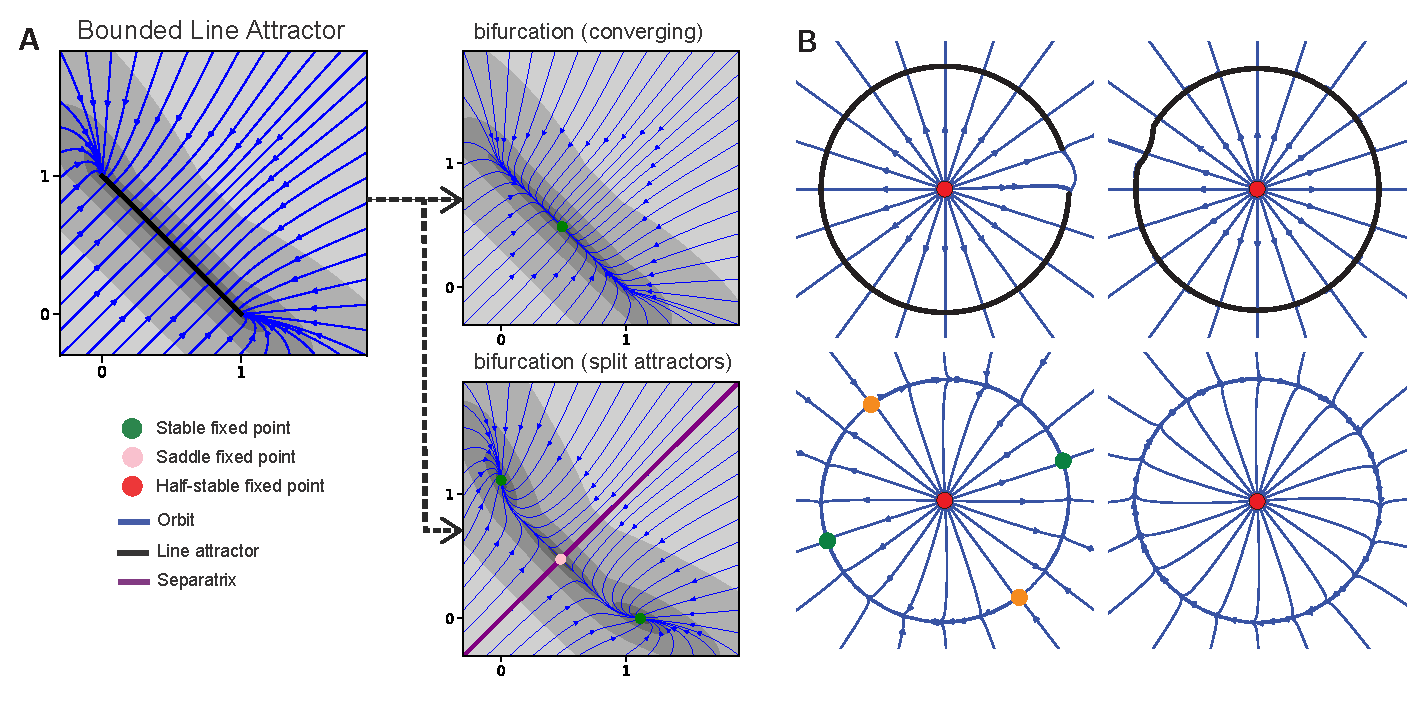
\includegraphics[width=\textwidth]{lara_bifurcations}
  \caption{The critical weakness of continuous attractors is their inherent brittleness as they are rare in the parameter space, i.e., infinitesimal changes in parameters destroy the continuous attractor implemented in RNNs~\cite{seung1996,Renart2003}.
  Some of the structure seems to remain; there is an invariant manifold that is topologically equivalent to the original continuous attractor.
    (A) Phase portraits for the bounded line attractor (Eq.~\eqref{eq:TLN}).
    Under perturbation of parameters, it bifurcates to systems without the continuous attractor.
    (B) The low-rank ring attractor approximation (Sec.~\eqref{sec:supp:lowrank}).
    Different topologies exist for different realizations of a low-rank attractor with overlap between the left and right vectors, different number of fixed points (4, 8 or 12) or a limit cycle (left bottom).
    Yet, they all share the existence of an ring invariant set.
}
\label{fig:lara_bifurcations}
\end{figure}

%par4: observation: CAs bifurcate into invariant manifolds topologically equivalent to the original CA
%Fig1

Ordinary differential equations (ODEs) are commonly used to describe the dynamical laws governing the temporal evolution of firing rates or latent population states\cite{vyas2020}.
In this framework, neural systems are viewed as implementing the continuous time evolution of neural states to perform computations.
We will consider a continuous attractor as a mechanism that implements analog memory computation: carrying a particular memory representation over time.
To define it formally, let $\vx(t) \in \reals^d$ denote the neural state, and $\dot{\vx} = \vf(\vx)$ represent its dynamics.
Let $\manifold \subset \reals^d$ be a manifold.
We say $\manifold$ is a continuous attractor, if (1) every state on the manifold is a fixed point, $\forall \vx \in \manifold, \vf(\vx) = 0$, and (2) the fixed points are marginally stable tangent to the manifold and stable normal to the manifold.
In other words, the continuous attractor is a continuum of equilibrium points such that the neural state near the manifold is attracted to it and on the manifold the state does not move.

For example, we can construct a line attractor (a continuous attractor with a line manifold) as follows:
%We will describe the bifurcation space of some continuous attractors.
%Neurons exhibit complex dynamics that can be described by differential equations.
\begin{align}\label{eq:TLN}
    \dot{\vx} = -\vx + \left[ \vW \vx + \vb \right]_{+}
\end{align}
where $\vW = [0, -1; -1, 0]$ and $\vb = [1; 1]$, and $[\cdot]_{+} = \max(0,\cdot)$ is the threshold nonlinearity per unit.
%where $\vx \in \reals^2$, $\vb \in \reals^2$ is the bias, $\vW \in \reals^{2\times 2}$ is the recurrent weight, and $[\cdot]_{+} = \max(0,\cdot)$ is the threshold nonlinearity per unit.
%In discrete time, this corresponds to a ReLU RNN (see Sec.~\ref{sec:rnn:integration}).
%The non-trivial activity of this network is limited to the (non-negative) first quadrant.
%The second kind of continuous attractor is created through negative feedback.
We get $\dot{\vx} = 0$ on the $x_1 = -x_2 + 1$ line segment in the first quadrant as the manifold (Fig.~\ref{fig:lara_bifurcations}A,left; black line).
We refer to it as the \emph{bounded line attractor} (BLA).
Linearization of the fixed points on the manifold exhibits two eigenvalues, $0$ and $-2$;
the $0$ eigenvalue allows the continuum of fixed points, while $-2$ makes the flow normal to the manifold attractive (Fig.~\ref{fig:lara_bifurcations}A,left; flow field).

Small changes to the parameters $(\vb,\vW)$ perturb the eigenvalues.
Specifically, any perturbation to the $0$ eigenvalue destroys the continuous attractor as it bifurcates to either
a single stable fixed point (Fig.~\ref{fig:lara_bifurcations}A top) or two stable fixed points separated with a saddle node in between (Fig.~\ref{fig:lara_bifurcations}A bottom).
However, interestingly, after bifurcation, continuous attractors seemingly tend to leave a ``ghost'' manifold topologically equivalent to the original continuous attractor (note the slow speed).
Furthermore, the vector field is not escaping the ghost manifold, i.e., it is an invariant manifold.
This phenomenon, wherein a continuous attractor is approximated by a manifold within the neural space along which the drift occurs at a very slow pace, has previously been commented on~\citep{seung1997learning,Mante2013-em}.
In general, continuous attractors are not only structurally unstable, they bifurcate almost certainly for an arbitrary perturbation.
In the following, we focus on 1-dimensional ring attractors.

%and perturbations cause the null eigenvalue to be non-zero and the line attractor disappears.
%However, surprisingly, the bifurcations are qualitatively different.
%Neither of these two cases show a divergent flow, but rather consists of one or two basins of attraction.
%It implies only vanishing gradients for this system and \textbf{exploding gradients will not be present for an arbitrarily long time}.

%The membrane potential of a neuron changes over time according to the input it receives and its intrinsic properties, which can be mathematically modeled using ODEs.
%Consider an RNN (without input or output for now) expressed in continuous time as an ordinary differential equation:
%A common form of the ODE for the firing rate \( r(t) \) of a neuron is:
%\begin{align}\label{eq:TLN2}
%\tau \frac{d r(t)}{d t} = -r(t) + F(I(t))
%\end{align}
%where:
%$\tau$ is the time constant of the neuron,
%$-r(t)$ represents the decay of the firing rate over time,
%$I(t)$ is the total input to the neuron at time \( t \) and
%$F(I)$ is a non-linear function that converts the input \( I(t) \) into an output firing rate.

% The Computation through Dynamics (CTD) framework assumes that the brain processes sensory information and generates behavior through neural dynamics, including representations of continuous-valued variables like space and direction~\cite{vyas2020}.

%Examples abound.

%When $d=2$ and $F(\cdot)= \max(0,\cdot)$ is the threshold nonlinearity, we can build a line continuous attractor as follows.
%First, through positive feedback, $\vW = [0, 1; 1, 0]$ and no bias $\vb = \mathbf{0}$, we can create a continuous attractor, i.e., $\dot{\vx} = 0$ on the $x_1 = x_2 \geq 0$ half-line, and surrounding attractive flow (Fig.~\ref{fig:ublabla}A left).
%We refer to it as an \textbf{unbounded line attractor (UBLA)}.
%For any point on the line attractor, linearization results in eigenvalues $0$ and $-2$, corresponding to the zero flow and attractive flow respectively.
%When $\vW$ is perturbed, the null eigenvalue can easily become non-zero and the continuous line attractor disappears.
%If it becomes negative, the system bifurcates to a stable fixed point at the origin (Fig.~\ref{fig:ublabla}A bottom).
%However, if it becomes positive (Fig.~\ref{fig:ublabla}A top), \emph{the resulting flow diverges to infinity along the diagonal}.
%Corresponding to the divergent flow, the backpropagating gradient over time exponentially grows in magnitude, thus rendering gradient descent impractical without truncation in time.
%
%any slight imperfections cause slow drift along the line This sort of approximate continuous attract or is what is found in real networks, including those trained by the learning
%``a manifold of stable fixed points'' \citep{Seung2000}.

\subsection{Theoretical models of ring attractors}\label{sec:ras}
% Furthermore, an invariant ring manifold with fixed points on it has been observed in finite dimensional low-rank attractors which converge to a ring attractor in the infinite unit limit~\citep{mastrogiuseppe2018,beiran2021}.
% We show some examples of such continuous attractor approximations in Fig.~\ref{fig:lara_bifurcations}B.
% Similarly, this has been observed in ring attractors with a finite number of units \citep{Noorman2022}, see also Fig.~\ref{fig:bio_rings}A.

%\subsubsection{Angular integration networks}\label{sec:hd}
For circular variables such as the goal-direction (e.g. for home navigation and working memory for communication	 in bees \citep{frisch1993dance}) %home navigation + dance in bees: the angle of the waggle phase relative to gravity reflects the angle of the food source relative to the sun
%duration of the waggle phse reflects the distance to the food source from the hive
or head-direction, the temporal integration and working memory functions are naturally solved by a ring attractor (continuous attractor with a ring topology) \citep{kim2019generation, turner2017angular, turner2020neuroanatomical,hulse2020mechanisms,taube2007head}.
Other examples include
integration of evidence for continuous perceptual judgments, e.g. a hunting predator that needs to compute the net direction of motion of a large group of prey \citep{esnaola2022flexible}.
In this section, we investigate the bifurcations of various implementations of continuous attractors.
Continuous attractor network models of the head-direction is based on the interactions of neurons that (anatomically) form a ring-like overlapping neighbor connectivity~\citep{zhang1996,Noorman2022,ajabi2023,vafidis2022,boucheny2005continuous,knierim2012}.
%Since continuous attractors are susceptible to noise and perturbations the precise representation of the head direction can in principle be disrupted easily.
Similarly as with the line attractor, the ring attractor bifurcates for virtually every perturbation.
Nevertheless, the bifurcated dynamics again follow a similar pattern of the dynamics restricted to the ghost manifold around the original continuous attractor.

\newcommand{\ptitle}[1]{\textbf{#1:}\xspace}
\ptitle{Piecewise-linear ring attractor model of the central complex}
Firstly, we discuss perturbations of a continuous ring attractor proposed as a model for the head direction representation in fruit flies~\citep{Noorman2022}.
This model is composed of $N$ heading-tuned neurons with preferred headings $\theta_j \in \{\nicefrac{2\pi i}{N}\}_{i=1\dots N}$ radians (see Sec.~\ref{sec:supp:headdirection}).
For sufficiently strong local excitation (given by the parameter $J_E$) and broad inhibition ($J_I$), this network will generate a stable bump of activity, one corresponding to each head direction.
This continuum of fixed points forms a one dimensional manifold homeomorphic to the circle.

\begin{figure}[tbhp]
     \centering
  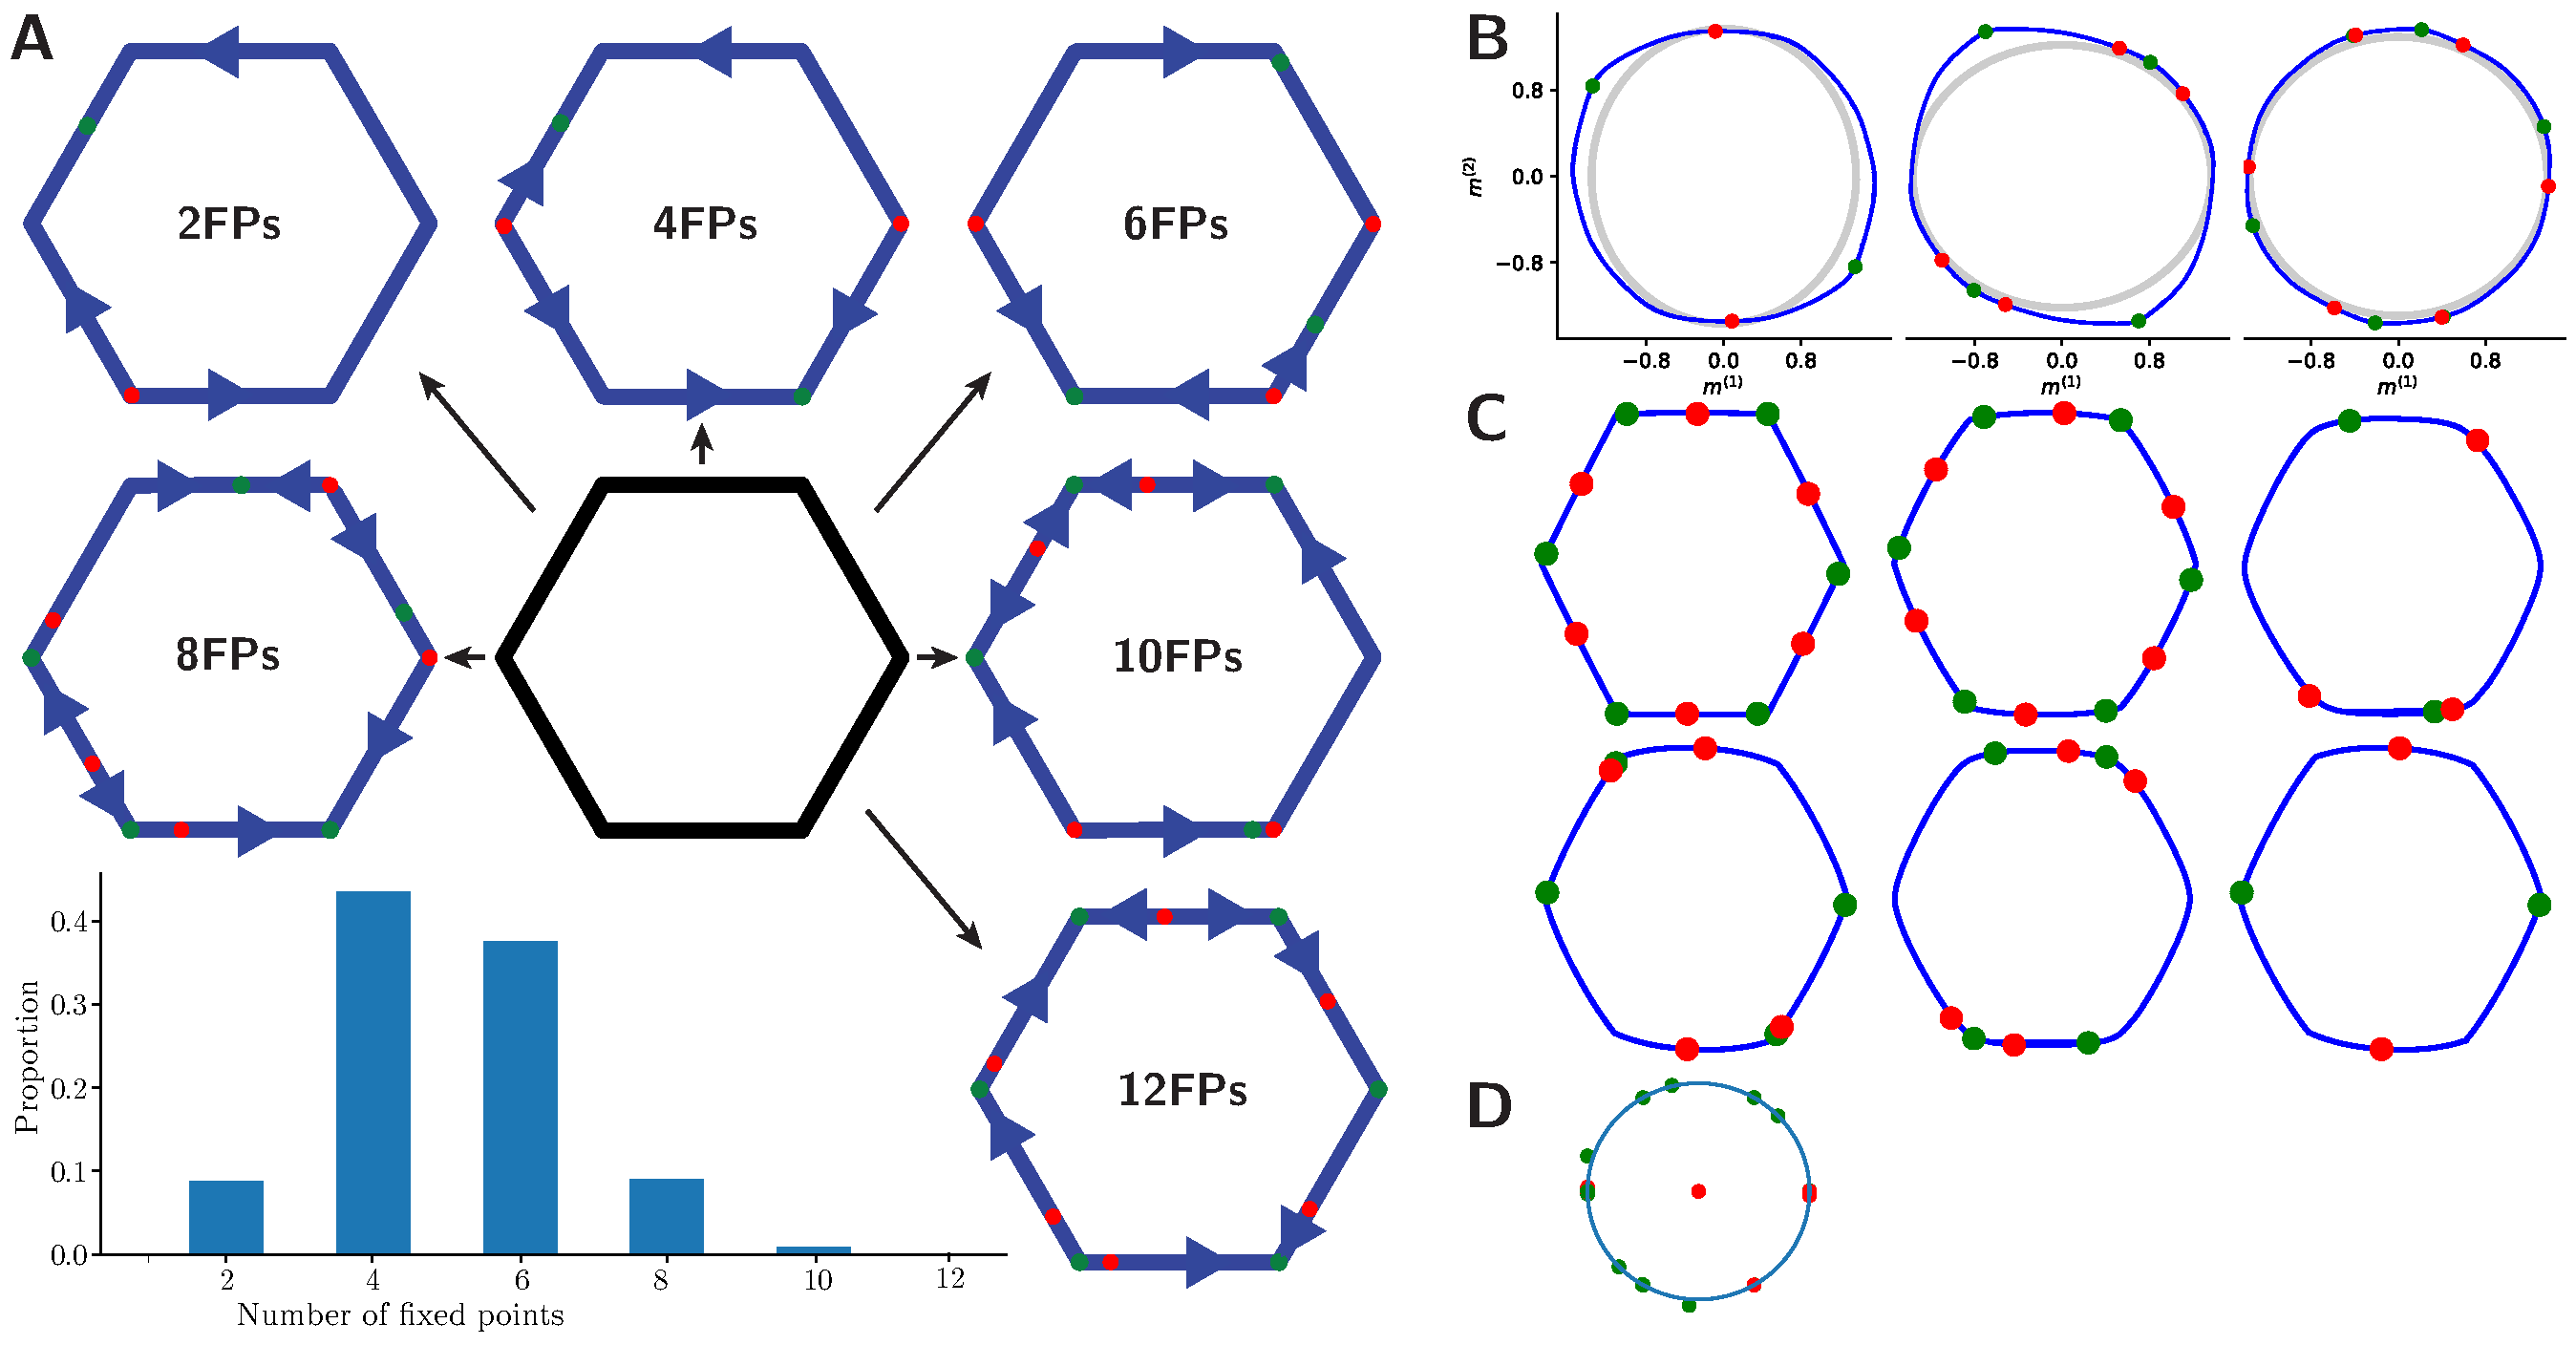
\includegraphics[width=\textwidth]{bio_rings}
       \caption{ Perturbations different implementation and approximations of ring attractors lead to bifurcations that all leave the ring invariant manifold intact. For each model, the network dynamics is constrained to a ring which in turn is populated by stable fixed points (green) and saddle nodes (red).
       (A) Perturbations to the ring attractor \citep{Noorman2022}. The ring attractor can be perturbed in systems with an even number of fixed points (FPs) up to $2N$ (stable and saddle points are paired). 
       (B)  Perturbations a low-rank approximation of a ring attractor \citep{mastrogiuseppe2018}.
       (C)  Perturbations to a tanh approximation of a ring attractor \citep{seeholzer2017efficient}.
       (D)  Different Embedding Manifolds with Population-level Jacobians (EMPJ) approximations of a ring attractor \citep{pollock2020}.
       }
         \label{fig:bio_rings}
\end{figure}

We evaluate the effect of parametric perturbations of the form $ \vW \leftarrow \vW + \vV$ with $\vV_{i,j}\iidsample\mathcal{N}(0,\nicefrac{1}{100})$ on a network of size $N = 6$ with $J_E= 4$ and $J_I=-2.4$ by identifying all bifurcations (Sec.~\ref{sec:supp:ring_perturbations}).
We found that the ring (consisting of infinite fixed points) can be perturbed into systems with between 2 and 12 fixed points (Fig.~\ref{fig:bio_rings}A).
As far as we know, this bifurcation from a ring of equilibria to a saddle and node has not been described previously in the literature.
The probability of each type of bifurcation was numerically estimated (See Sec.~\ref{sec:supp:headdirection}).
There are several additional co-dim 1 bifurcations with measure zero (see Fig.~\ref{fig:meaure_zero_perturbations}).
%The space of possible perturbations in Sec. ~\ref{sec:imt} is very large. To be able to form an image of what happens in the theorem we will work out the effect of some examples of perturbations.

%how can we understand the underlying mechanism of these bifurcations

%\mpcomment{transition missing}
%In modeling neural dynamics, ensuring biological plausibility is paramount.
\ptitle{Bump attractor model}
%A well-established approach, consistent with the principles observed in the fly head direction network \citep{kakaria2017}, involves utilizing 
%a circulant matrix as the connectivity matrix\citep{samsonovich1997path, seeholzer2017efficient, redish1996coupled, goodridge2000, compte2000synaptic}.
The infinite sized ring attractor network can support a stable ``activity bump'' that can move around the ring in correspondence with changes in head direction.
%The position of this bump encodes the head direction.
This can be accomplished with a connection matrix $W$ with entries that follow a circular Gaussian function of $i-j$ \citep{seeholzer2017efficient,redish1996coupled,goodridge2000,compte2000synaptic}.
For finite sized networks the dynamics is constrained to an attractive invariant ring, covered with $N$ stable fixed points for a networks of size $N$ (Fig.~\ref{fig:bio_rings}C).
%
%Furthermore, our theory indicates that the reason why networks of generic spiking neurons with connectivity inferred from light-resolution microscopy gives rise to approximate ring attractors\citep{kakaria2017}, is because they are nearby ring attractors as dynamical systems.

\ptitle{Low-rank ring attractor model} %mastrogiuseppe, beiran, ostojic
Low-rank networks can be used to approximate ring attractors~\citep{mastrogiuseppe2018, beiran2021}.
Using dynamical mean field theory, in the limit of infinite-size networks, one can construct a ring attractor through a rank 2 network by constraining overlap of the right- and left-connectivity vectors. \mpcomment{add link to details}
However, in simulations of finite-size networks with this constraint, the dynamics instead always converge to a small number of stable fixed points located on a ring~\citep{mastrogiuseppe2018}.

\ptitle{Embedding Manifolds with Population-level Jacobians} %pollock, jazayeri
Approximate ring attractors can be fit by constraining the connectivity so that the networks Jacobian satisfies certain necessary requirements for a ring attractor to exist (Sec.~\ref{sec:supp:empj}~\citep{pollock2020}).
The fitted models through this method also contain an invariant ring manifold on which the dynamics contains stable and saddle fixed points.

\ptitle{Remark}
In all example models of ring attractors, we verify that they suffer from the fine-tuning problem.
We have observed the ghost of the continuous attractors in many different systems (either through bifurcation or from finite-size effects): an attractive invariant manifold.
Is this a universal phenomenon?
Moreover, although the exact ring attractor was not implemented, they were approximate ring attractors in some sense.
Are continuous attractors somehow still useful as a model of how animals might represent continuous variables?
We will answer these questions in an implementation-agnostic manner.

% Our theory explains this phenomenon as follows. %MOVE TO LATER
% We can think of the finite size realization as a small perturbation to the infinite size network on the reduced dynamics in the $m^1, m^2$ plane (independent of the parameter $g$ for the random part of the matrix)  (Fig.~\ref{fig:bio_rings}B).
% %This implies that the ring attractor network 
% For very small networks the ring structure is destroyed and only the plane persist as a slow manifold.

%\mpcomment{are we going to describe EMPJ here?}
%how to show 
%normal hyperbolicity index: speed normal/tangent to manifold
%fenichel brakes down
%uniform bound approximation
%Is this only true for ReLU parameterized RNNs, or does it generalize?

%In this paper, we lay out a new theory of general continuous-valued memory to answer the following questions:
%\begin{enumerate}
%%    \item Can we avoid exploding gradients under parameter perturbation?
%    \item Do we need to worry about the brittleness of the continuous attractor solutions in practice?
%    \item Are continuous attractors useful as a model of how animals might represent continuous variables?
%    %How can biological networks approximate the representation of continuous variables?
%\end{enumerate}
%\mpcomment{These are good questions to be embedded in the text. Probably not as bullet points? Not sure.}
%Our theory provides answers to both questions under mild assumptions in an architecture agnostic manner.
%Using Fenichel's invariant manifold theorem, we derive a sufficient condition for RNNs implementing continuous attractors to remain free of exploding gradients.
%Moreover, even after a bifurcation, these RNNs still approximately behave like the original continuous attractor (for a while).

%Using Fenichel's invariant manifold theorem, we derive a universality statement for the bifurcation landscape for one dimensional continuous attractors:
% the behavior of one-dimensional continuous attractors can be effectively described by slow ring manifolds.
% These manifolds can either take the form of collections of stable fixed points and saddle points with connecting orbits or that of a limit cycle. 
% This characterization provides a fundamental understanding of a continuous attractors bifurcation landscape.
%%what is uni statement?
%We verify our theoretical insights with numerical experiments.
%We show that all approximations, whether it is trained RNNs or hand designed contintuous attractors, are all to be described as slow manifolds with the same topology as the original continuous attractor,
%%punchlines
%even though they differ from each other in terms of the topology of the dynamics (e.g. number of fixed points).


%\section{Theory of gracefully degrading continuous attractors}\label{sec:theory}
\section{Theory of Approximate Continuous Attractors}\label{sec:theory}
%In this section, we apply invariant manifold theory to RNNs and translate the results for the theoretical neuroscience audience.
%Our emphasis in this paper centers on investigating the distinctive properties of continuous attractors that prove essential for specific tasks, with a deliberate exclusion of considerations related to learning chaotic dynamics.
%\subsection{Invariant Continuous Attractor Manifold Theory}\label{sec:imt}
\subsection{Persistent Manifold Theorem}\label{sec:imt}
%We start by formulating an ODE implementing a continuous attractor in continuous time: $\dot{\vx} = \vf(\vx)$.
Let $l$ be the intrinsic dimension of the manifold of equilibria that defines the continuous attractor.
Given a perturbation to the ODE $\vp(\vx)$ that induces a bifurcation,
\begin{align}\label{eq:perturbation:nonparam}
	\dot{\vx} &= \vf(\vx) + \epsilon\,\vp(\vx)
\end{align}
where $\uniformNorm{\vp(\cdot)} = 1$ and $\epsilon > 0$ is the bifurcation parameter,
we can reparameterize the dynamics around the manifold with coordinates $\vy \in \reals^l$ and the remaining ambient space with $\vz \in \reals^{d-l}$.
To describe an arbitrary bifurcation of interest, we introduce a sufficiently smooth function $g$ and $h$, such that the following system is equivalent to the original ODE:
\begin{align}\label{eq:fenichel:flow}
    \dot{\vy} &=           \epsilon  \vg(\vy, \vz, \epsilon) \qquad \text{(tangent)}\\
    \dot{\vz} &= \hphantom{\epsilon} \vh(\vy, \vz, \epsilon) \qquad \text{(normal)}
\end{align}
where $\epsilon = 0$ gives the condition for the continuous attractor $\dot{\vy} = \mathbf{0}$.
We denote the corresponding manifold of $l$ dimensions $\manifold_0 = \{(\vy,\vz) \mid \vh(\vy,\vz,0) = 0\}$.

We say the flow around the manifold is \emph{normally hyperbolic}, if the flow normal to the manifold is hyperbolic, meaning that the Jacobians $\nabla_\vz \vh$ evaluated on any point on the $\manifold_0$ has $d-l$ eigenvalues with their real part uniformly away from zero, and $\nabla_\vy \vg$ has $l$ eigenvalues with zero real parts.
More specifically, for continuous attractors, the real part of the eigenvalues of $\nabla_\vz \vh$ will be negative, representing sufficiently strong attractive flow toward the manifold.
Equivalently, for the ODE, $\dot{\vx} = \vf(\vx)$, the variational system is of constant rank, and has exactly $(d-l)$ eigenvalues with negative real parts uniformly away from zero and $l$ eigenvalues with zero real parts everywhere along the continuous attractor.
Informally, normal hyperbolicity guarantees that the perturbations changes the structure of the manifold before they can destroy the attractiveness of the manifold.

\begin{SCfigure}[10][bthp]
  \centering
  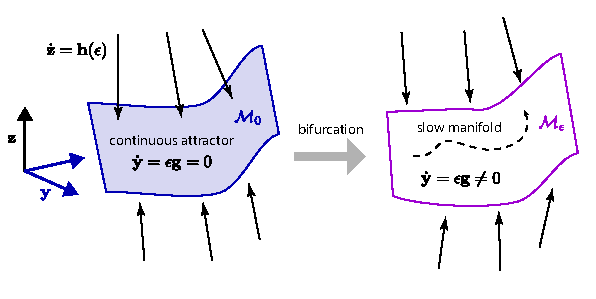
\includegraphics[width=0.5\textwidth]{FenichelThm}
  \caption{
    Persistent manifold theorem applied to compact continuous attractor guarantees the flow on the slow manifold $\manifold_\epsilon$ is locally invariant and continues to be attractive.
    The dashed line is a trajectory ``trapped'' in the slow manifold (locally invariant). %change to forward invariant?
    %mention topology?
  }
  \label{fig:fenichel}
\end{SCfigure}

When $\epsilon > 0$, the continuous attractor bifurcates away.
What can we say about the fate of the perturbed system?
The continuous dependence theorem~\citep{Chicone2006} says that the trajectories will change continuously as a function of $\epsilon$ without a guarantee on how quickly they change.
Moreover, the topological structure and the asymptotic behavior of trajectories change discontinuously due to the bifurcation.
Surprisingly there is a strong connection in the geometry due to Fenichel's theorem~\cite{fenichel1971}.
We informally present a special case due to~\citet{Jones1995}:
\begin{theorem}[Persistent Manifold Theorem]
Let $\manifold_0$ be a connected, compact, normally hyperbolic manifold of equilibria originating from a sufficiently smooth ODE.
For a sufficiently small perturbation $\epsilon > 0$, there exists a manifold $\manifold_\epsilon$ diffeomorphic to $\manifold_0$ and locally invariant under the flow of \eqref{eq:fenichel:flow}.
Moreover, $\manifold_\epsilon$ has $\mathcal{O}(\epsilon)$ Hausdoff distance to $\manifold_0$ and has the same smoothness as $g$ and $h$. % in (\ref{eq:fenichel:flow}).
\end{theorem}

The manifold $\manifold_\epsilon$ is called the \emph{slow manifold} which is no longer necessarily a continuum of equilibria.
However, the local invariance implies that trajectories remain within the manifold except potentially at the boundary.
Furthermore, the non-zero flow on the slow manifold is slow and given in the $\epsilon \to 0$ limit as $\RN{\vy}{\tau} = \vg(c^\epsilon(\vy), \vy, 0)$ where $\tau = \epsilon t$ is a rescaled time and $c^\epsilon(\cdot)$ parameterizes the $l$ dimensional slow manifold.
In addition, the stable manifold of $\manifold_0$ is similarly  persistent~\cite{Jones1995}, implying the manifold $\manifold_\epsilon$ to remain attractive.


These conditions are met for the examples in Fig.~\ref{fig:lara_bifurcations} (see Sec.~\ref{sec:supp:fast_slow_form} for the rerparametrization of the BLA).
 As a technical note, for the theory to apply to a continuous piecewise-linear system, it is required that the invariant manifold is globally attracting \cite{simpson2018}, which is also the case for the BLA.
%applicability of Fenichel’s invariant manifold theorem on continuous piecewise linear (PWL) dynamical systems.
As the theory predicts, BLA bifurcates into a 1-dimensional slow manifold (dark colored regions) that contains fixed points, and is overall still attractive.
%On the contrary, the UBLA does not satisfy the compactness condition, hence the theory does not predict its persistence. %extension: 
%Importantly, the ``slow'' flow on the perturbed system is not bounded.

Fenichel's Persistent Manifold theorem explains the bifurcation structure of the theoretical models discussed in Sec.~\ref{sec:ras}.
As continuous ring attractor are bounded, their invariant manifold persists and it remains attractive under small perturbations to this system~\citep{wiggins1994}.
%Furthermore, because the ring attractor is boundaryless %it is both forward and backward invariant, i.e. hence
%the persistent manifold is invariant ~\citep{wiggins1994}.

%Given an $d$-dimensional continuous attractor manifold embedded within a recurrent dynamics of $n$-dimensions, it supports persistent continuous memory of $d$-dimension.
%There are $d$ zero Lyapunov exponents corresponding to the perturbations tangent to the manifold, coinciding with the memory representation, and $(n-d)$ negative Lyapunov exponents that expresses the attractive nature.
%In theory, the topology of the manifold can be arbitrary, ideally matching the desired structure of the target variables.

%In practice, the sufficient conditions for RNNs implementing continuous attractors to have this graceful breakdown (like BLA but not UBLA) is for the continuous attractor manifold to be of finite dimension throughout, connected, and bounded.
%However, in systems with an invariant manifold with dimension at least three, it is possible that a slow manifold with chaotic dynamics is created through a perturbation.
%This would have as consequence that the perturbed system acquires positive Lyapunov exponents (corresponding to the chaotic orbit), which then can still lead to exploding gradients albeit with very slow flow that has little practical consequence in finite time experiments.
%The probability of such a bifurcation is low.


%\subsection{Implications on Machine Learning}\label{sec:imp:ML}
%Extending the memory time constant of RNNs have long been an important area of research with much focus on random weights~\cite{Legenstein2007,Goldman2009,Toyoizumi2011,Kerg2019,Chen2018,Henaff2016,Rusch2021,arjovsky2016}.
%Various initializations for the recurrent weights have been proposed to help learning: initialization with the identity matrix \citep{le2015}, with a random orthogonal matrix \citep{saxe2014,Henaff2016}, with a unitary matrix \citep{arjovsky2016} and with a block diagonal weight matrix that creates a quasi-periodic system with limit cycles \citep{Sokol2019a}.
%However, despite the capacity to maintain representation of continuous quantities for arbitrary duration of time, continuous attractor mechanism has not been pursued in machine learning research because of its brittleness.
%The stochasticity in gradients inherited from the training data, regularization strategy, and multi-task learning objectives act as a perturbation on the recurrent dynamics, and continuous attractors break down even if it could be learned.
%Remedies emerged in machine learning to hard-code continuous-valued memory structures within the RNNs---e.g., the cell state in vanilla LSTM.
%However, our theory shows that the geometric structure of the manifold and the flow around the manifold play a critical role in enabling gradient descent learning of continuous attractors using standard methods such as backpropagation through time (BPTT)~\cite{Toomarian1991}. 
%
%It is well known that asymptotic exploding gradients comes from positive Lyapunov exponents~\cite{Mikhaeil2022,Vogt2022,Engelken2023}.
%It has also been pointed out that bifurcations can cause arbitrarily large gradients~\cite{doya1993} as well as discontinuity in the Lyapunov spectrum~\cite{Park2023a}.
%These gradient propagation theories suggested that bifurcations should be avoided, including the continuous attractors.
%
%As far as we know, there is no architecture agnostic theory describing the loss landscape around RNN solutions.
%We remark that due to the singular nature of the center manifold that supports the continuous attractor, the usual analysis approach of linearization fails.
%\emph{Our theory successfully connects the invariant manifold theory and the gradient signal propagation theory in RNNs to describe two types of loss landscape around continuous attractor solutions.}
%In one case, when the theorem holds, the landscape is shallow in all directions due to (asymptotically) vanishing gradients induced by the attractor structure---we have the gracefully degrading continuous attractor.
%In the other case, we can find examples where the theorem does not hold, and the continuous attractor solution is at the boundary of network configurations with exploding gradients, meaning the loss landscape is very steep in some directions.
%While exploding gradients would prevent gradient descent to correct for deviations from the optima,
%for gracefully degrading ones, one can apply restorative forces via gradient descent to be in the vicinity of the brittle continuous attractor solution (see Sec.~\ref{sec:exp:maintaining}).

\subsection{Fast-Slow decomposition and the revival of continuous attractors}\label{sec:revival}
Consider a behaviorally relevant time scale for analog working memory, for instance, 10 ms to 10 sec.
If the dynamical system is orders of magnitude slower, for example, 1000 sec or longer, its effect is too slow to have a practical impact on the behavior that relies on the working memory mechanism.
This clear gap in the fast and slow time scales can be recast as \emph{extended normal hyperbolicity} of the slow manifold by relaxing the zero real part to a separation of time scales (reciprocal of eigenvalues or Lyapunov exponents).
In other words, the attractive flow normal to the manifold needs to be uniformly faster than the flow on the manifold.

By taking the limit of the slow flow on the manifold to arbitrarily long time constant (i.e., to zero flow), we achieve the reversal of the persistent manifold theorem.
\begin{prop}[Revival of continuous attractor (informal)]\label{prop:revival}
Let $\manifold_\epsilon$ be a connected, compact, slow manifold with extended normal hyperbolicity. % in the neighborhood of a continuous attractor.
Let the uniform norm of the flow tangent to the manifold be $\eta$.
There exist a perturbation with uniform norm at most $\eta$ that induces a bifurcation to a continuous attractor manifold $\manifold_0$ diffeomorphic to $\manifold_\epsilon$.
\end{prop}

The uniform norm of vector field on the manifold is a useful measure of distance from a continuous attractor.
It can also be used to bound the memory performance on the short-time scale. % based on the uniform bound of the slow flow.
Let $\vx_0 \in \manifold$, and $\phi = \vp\vert_\manifold$ be the flow restricted to the manifold.
The average deviation from initial memory $\vx_0$ over time is bounded linearly
\begin{align}\label{eq:distance:ub}
\frac{1}{\manifold}\int_\manifold
%\frac{1}{T}\int_0^T
\abs{\vx(t, \vx_0) - \vx_0}\,
%\dm{t}
\dm{\vx_0}
\leq t\uniformNorm{\phi}
\end{align}

\subsection{Relevance of dynamics on the slow manifold in the asymptotic time scale}\label{sec:attractor_bif}
While the uniform norm gives insight into short time scale behavior, we can expect that working memory tasks generalize to longer durations~\citep{Park2023a}.
Long-time scale behavior of the slow manifold is dominated by the stability structure, i.e., the topology of the dynamics.
Although we have seen numerous topologies in Sec.~\ref{sec:critique}, dynamical systems theory says that they are fundamentally limited, especially in low-dimensions.
%Understanding attractors and their bifurcation structure is crucial in neuroscience because they provide a blueprint for how neural activity can remain stable and robust even in the face of disruptions.
%This resilience is fundamental for cognitive functions, learning, and memory. 
%Thanks to Fenichel's Persistent Manifold Theorem, we can understand how these persistent pathways, or manifolds, survive even when the system undergoes  bifurcations.
%Essentially, this theorem assures us that the underlying structure of continuous attractors remains intact, maintaining a consistent topology despite the changes.
%The theory implies that in the space of dynamical systems, all systems in the neighbourhood of a continuous attractor all share the same topology for the attractive persistent invariant manifold and that the flow on the manifold is slow.
For a ring attractor this implies that the stability structure of the invariant manifold is either
(1) composed of an equal number of stable fixed points and saddle nodes, placed alternatingly and with connecting orbits, or (2) a limit cycle.
%saddle node with homoclinic orbit: with noise equivalent to a limit cycle
For 2 dimensional attractors stable fixed points and saddle nodes can coexist with limit cycles.
In more complex scenarios, such as a two-dimensional attractor, stable fixed points and saddle nodes can coexist with limit cycles, creating a rich tapestry of possible neural states.
For example, the dynamics on a torus manifold can be described by Kolmogorov-Arnold-Moser (KAM) theory.
%For higher dimensional attractors, there is the possibility of chaos emerging, but we conjuncture that the bifurcations leading to such behavior are a measure zero set.
%\mpcomment{refer to later section on generalization performance?}

%No matter the dimension, the essential takeaway is that there will always be an attractive invariant manifold that mirrors the topology and dimension of the original continuous attractor.
%This means that, even with perturbations, neural states aren't drastically altered from where they would have been, maintaining a semblance of the original flow.
% the compact case: the invariant manifolds are diffeomorphic to the original one. So neural states aren’t too far off from where they would have been before the perturbation.
%\mpcomment{This subsection is very dry. Make it sound cool and also explain why these are important considerations in the context of neuroscience.}

\section{Numerical Experiments on Task-optimized Recurrent Networks}\label{sec:experiments}
% Continuous attractor approximations} %from trained RNNs

While our theory describes the abundance of approximate continuous attractors in the vicinity of a continuous attractor, it does not imply that there are no approximate solutions away from continuous attractors.
We use task-optimized recurrent neural networks (RNNs) as means to searching for plausible solutions for analog memory with ring topology.
We will train a diverse set of RNNs, then identify the solution type of trained RNNs to gain insights into its performance, error patterns, generalization capabilities, and, ultimately, proximity to a continuous attractor.
%Recurrent neural networks (RNNs) are universal approximators of dynamical systems \citep{doya1993, schafer2006recurrent} and should therefore be able to approximate continuous attractors. \mpcomment{I disagree that it is!! It is a universal approximators of bounded length sequence-to-sequence transformations, not dynamical systems. Guillermo?}
%Leveraging a fast-slow decomposition methodology, premised on the assumption of normal hyperbolicity within the system, we first identify the slow manifold through a velocity bound criterion, and then identify the slow flow by its asymptotic behavior.


Understanding the implemented computation in neural systems in terms of dynamical systems has a well-established practice~\citep{seung1996,sompolinsky1988}.
Researchers have attempted to understand optimized neural networks through nonlinear dynamical systems analysis~\citep{sussillo2013blackbox,sussillo2014,barak2013,driscoll2022,maheswaranathan2019universality,cueva2019headdirection,cueva2021continuous} and to compare those artificial networks to biological circuits~\citep{mante2013context,remington2018flexible,ghazizadeh2021slow}.
% 
Previously, systematic analysis of the variability in network dynamics has been surveyed in vanilla RNNs and variations in dynamical solutions over architecture and nonlinearity have been quantified~\citep{sussillo2013blackbox,mante2013context,yang2019task,maheswaranathan2019universality,driscoll2022}.
Furthermore, the spectrum of how RNNs may hold memory has been addressed~\citep{orhan2019diverse}.
%comparing artificial network representations to neural data
We therefore investigated to what extent training RNNs on a task uniquely determines the low-dimensional dynamics, independent of neural architectures.

\subsection{Model Architectures and Training Procedure}
We examined vanilla continuous-time RNNs for this work.
The time discretized version of RNN network activity is given by
\begin{equation}
  \begin{aligned}
	\vx_t &= f(\win \vI_t + \vW \vx_{t-1} + \vb) + \zeta \label{eq:RNN:discrete}\\
	\vy_t &= \wout \vx_t + \bout
  \end{aligned}
\end{equation}
where $\vx_t \in \reals^d$ is the hidden state, 
$\vy_t $ is the readout, 
$\vI_t \in \reals^K$ is the input,
$f\colon \reals \to \reals$ an activation function which acts on each of the hidden dimension, 
private noise variable $\zeta\sim\mathcal{N}(0,\nicefrac{1}{100})$, and %$\zeta\sim \mathcal{N}(0, .001)$
$\vW, \vb, \win, \wout, \bout$ are parameters.
Assuming an Euler integration with unit time step, the discrete-time RNN of \eqref{eq:RNN:discrete} corresponds to the stochastic differential equation:
\begin{align}
    \dm{\vx} &= -\vx\dm{t} + f(\win \vI + \vW \vx + \vb)\dm{t} + \sigma \dm{W}. \label{eq:RNN:continuous}
\end{align}
where $\dm{W}$ is Wiener process that models the intrinsic state noise in the brain.

Building upon prior work, which has shown networks' capabilities on such tasks, we trained RNNs to either
(1) estimate head direction through integration of angular velocity \citep{cueva2019headdirection, cueva2021continuous}
and (2) perform a memory guided saccade task for a ring variable \citep{wimmer2014} (details in Sec.~\ref{sec:supp:tasks}).
The loss $L$ to be minimized was computed by mean squared error (MSE) between the network output $y(t)$ and the target output $\hat y(t)$.
\begin{equation}\label{eq:loss}
L_{MSE} \coloneqq \langle m_{i,t}(y_{i,t}-\hat y_{i,t})^2\rangle_{i,t}
\end{equation}
with $i$ the index of the output units and $t$  the index for time.
We implemented a mask, $m_{i,t}$, for modulating the loss with respect to certain time intervals.


We trained 10 networks for every combination of the following parameters:
 ReLU, tanh and rectified tanh activation functions and
 number of units/neurons (32, 64, 128, 256).
% , and activity regularization ($10^{-3}, 0, 1$).
%
All networks were trained using ADAM with $\beta_1=0.9$ and $\beta_2=0.999$ for $5,000$ iterations with a batch size of 64. % and a stopping criterion............. % and training was run until no decrease in the loss occurred for 100 epochs
%Among the networks, we only analyzed networks with normalized MSE less than -20 dB (Fig.~\ref{}).

%To avoid overly complex solutions that do not generalize well for longer trials, we penalized high activity using an L2 regularization on the hidden activity $x_t$.
%%We trained networks with regularizer
%The hyperparameter selection criterion for regularization was the highest level of regularization that ...............
%We found the highest level regularization that ...............


%\subsection{Fast-slow decomposition: Unpacking the slow manifolds in trained RNNs} %from trained RNNs
% separate the time scales to obtain the fast flow normal to the ``ghost'' continuous attractor (a.k.a. slow manifold) and the slow flow within
%intro:
%-goal: to identify the solution type of a trained RNN + understand it's performance/errors/generalization/closeness to a CA
%-how through a fast-slow decomposition, based on the assumption that there is normal hyperbolicity in the system  


 %method
\subsection{Numerical Fast-Slow Decomposition}\label{sec:fastslowmethod}
For each trained network, we find the slow manifold  by integrating the autonomous dynamics and we select the parts of the trajectory that have speed slower than a threshold.
%
%We assess the intrinsic dimensionality of the manifold with the Method Of Moments algorithm \citep{amsaleg2018extreme, altan2021estimating}.
In the cases that we identify a one dimensional invariant manifold $\manifold$, we parametrize it by fitting a cubic spline with periodic boundary constraints to these points (black line in Fig.~\ref{fig:fastslow_decomposition}A and B).
Alternatively, we identify the points along the trajectories that are the closest to a set of point in the output space relevant to the task after convergence, i.e. on the unit ring.
%Finally, we find the stable fixed points through a threshold on the 
Finally, we find the fixed points on the invariant ring by identifying regions where the direction of the flow flips for a dense set of points on the found invariant manifold.
We assess the direction through projection onto the output mapping and calculating the angular flow.
Stable fixed points are identified where the flow directions are both pointing towards this flip point, 
while saddle nodes are identified wherethey are pointing away (filled and hollow circles Fig.~\ref{fig:fastslow_decomposition}A and B for stable and saddle fixed points respectively).
We find that long integrated trajectories of the network converge to the found stable fixed points through this independent method.


\subsection{Variations in the Topologies of the Networks}\label{sec:topologies}
In this section, we dissect the dynamics of RNNs by segregating time scales to delineate the rapid flow normal to the slow manifold, and the flow on the manifold.
We want to investigate how networks might solve tasks.
%While previous studies have primarily focused on simple tasks that can be solved with fixed points, there remains a gap in comprehensively extracting the mechanisms underlying network implementations~\citep{sussillo2013blackbox}.
%We address this gap by investigating the internal mechanisms of neural network solvers for tasks involving continuous variables.

%Fig 4
\begin{figure}[tbhp]
  \centering
  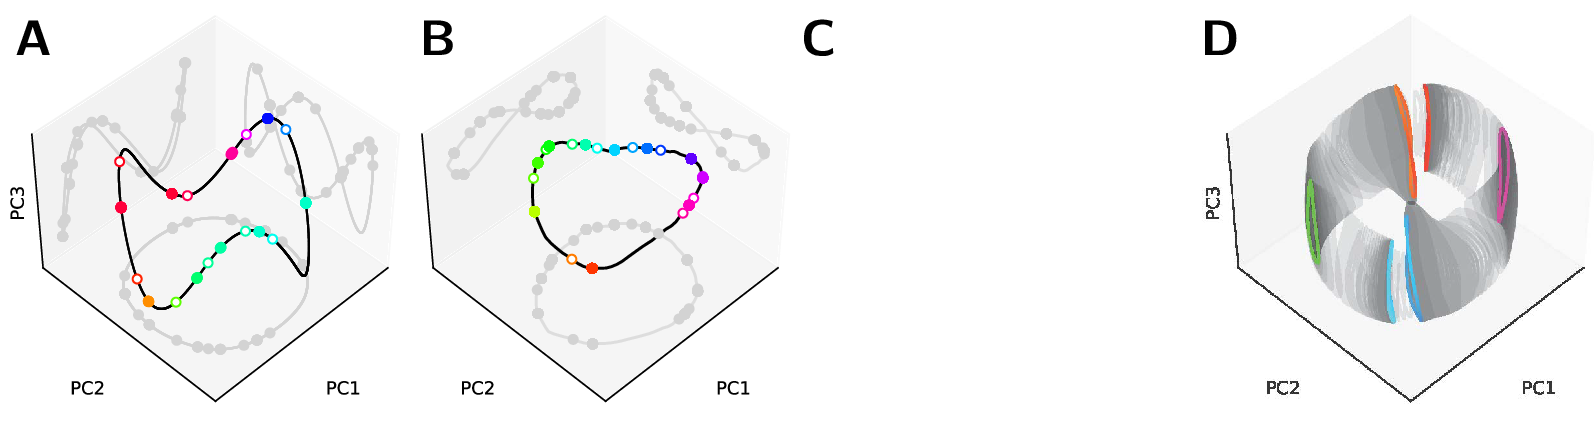
\includegraphics[width=\textwidth]{fastslow_decomposition}
  \caption{Slow manifold approximation of different trained networks on the memory guided saccade and angular velocity integration tasks.
 (A1) Example of a trajectory on the  angular velocity integration task.
 (A2) Example of a trajectory on the  memory guided saccade task.
 (B) An example fixed point type solution to the memory guided saccade task.
 (C) An example found solution to the angular velocity integration task.
 (D) An example slow torus type solution to the memory guided saccade task. The colored curves indicate stable limit cycles of the system.
}
  \label{fig:fastslow_decomposition}
\end{figure}

All solutions involve a slow manifold with the same topology as the relevant variable in the task.
The different solutions are different in their asymptotic dynamics (Fig.~\ref{fig:fastslow_decomposition}).
The most often found solution is of the type \emph{fixed point ring manifold} (Fig.~\ref{fig:fastslow_decomposition}A and B).

Less commonly found topologies include slow limit cycles (Fig.~\ref{fig:fastslow_decomposition}C) and a slow torus around a repulsive ring invariant manifold (Fig.~\ref{fig:fastslow_decomposition}D).
These solutions are consistent with both observations of the possibility of using non-constant dynamics for memory storage~\citep{hirsch1995computing,Park2023a} and neuronal circuits underlying persistent representations despite time varying activity~\citep{druckmann2012neuronal}.

\subsection{Universality amongst Good Solutions}
%to what extent does training neural networks to solve simple tasks, prevalent in neuroscientific studies, uniquely determine the low-dimensional dynamics independent of neural architectures?
%are the learned dynamics highly sensitive to different neural architectures?

The fixed point topologies show a lot of variation across networks (Fig.~\ref{fig:fastslow_decomposition}A and B),
 much like the systems next to continuous attractors (Fig.~\ref{fig:lara_bifurcations} and Fig.~\ref{fig:bio_rings}).
Previously, it has been observed that  fixed point analysis  has as a major limitation, namely, that the number of fixed points must be the equal across compared networks  \citep{maheswaranathan2019universality}.
Our methodology effectively addresses and overcomes this limitation.
The universal structure of continuous attractor approximations as slow invariant manifolds allows us to connect different topologies as \textbf{approximate continuous attractors} (Sec.~\ref{sec:attractor_bif}).

% \subsection{Infinite horizon computation in a bounded state space}\label{sec:inhoco}
% Both sequential and nearly persistent solutions are part of a spectrum that emerges naturally in trained networks under different conditions~\citep{orhan2019diverse}.
% %We describe the general implementational principles of robust, timing-independent (infinite horizon) neural computation.
% If a dynamical system is implementing a timing-independent (infinite horizon) computation, on a compact domain, the state will evolve to an attractor state inside the chain-recurrent recurrent set~\citep{conley1978}.
% This implies that the only possible implementation of a continuous valued memory that can be decoded linearly is the (approximate) continuous attractor.

% \mpcomment{move the following to the end or conclusion}
% Through a series of experiments of training RNNs on two tasks with various architectures, sizes and activation functions, we shed light on the intricate workings of neural networks when confronted with continuous-variable tasks.
% Amidst the variability of solutions, we observe that all trained networks share the universal feature of having a slow invariant manifold with the same topology as the variable on which the computation relies.
% This empirical evidence strongly corroborates our proposed theory of continuous memory.




\section{Generalization Analysis}

%distinct topology of these dynamics implies qualitatively different behaviors in the asymptotic limit of time

Animals are trained on a task for finite time and it is therefore unclear that they learn the intended computation or just a finite time approximation of it.
The same is the case for the trained networks.
We will investigate to what extent the networks have the intended memory necessary for the task or whether they implement it on the timescale on which they have been trained.

%Our theory shows that not all continuous attractors are born equal, and that there are gracefully degrading continuous attractors.
%In finite time, trajectories are well-behaved, contrary to the asymptotic behavior captured by the Lyapunov exponents.
%Animal behavior is finite time in nature and the longer the temporal distance the harder it is to learn temporal dependencies in general.

%generalization
%\subsection{Different topologies have different generalization properties}
\subsection{Generalization properties of continuous attractor approximations}\label{sec:generalization}
%, and thus a corresponding pattern of error in temporal generalization

The two possible approximations of a ring attractor discussed in Sec.~\ref{sec:critique} exhibit markedly distinct generalization characteristics.
Approximating the system as a limit cycle results in memory that gradually diminishes over time.
Conversely, the alternative approximation's memory states are contingent upon the quantity and positioning of stable fixed points within the system.
We will in detail describe the generaralization properties of the trained networks on the angular velocity integration task.
We tested all networks with a validation set and took a cutoff for the normalized MSE for the networks we consider for the analysis at -20 dB (Fig.~\ref{fig:angular_loss}C).

Looking beyond the finite timescale provides valuable insights into the network's ability to store information.
% and how this ability degrades across different perturbations.
We want in particular to investigate the angular memory capacities of the trained networks.
We will assess this capacity at two different time-scales:  asymptotic and finite time.


\begin{figure}[tbhp]
  \centering
  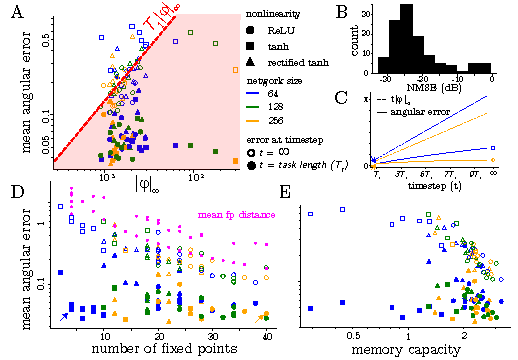
\includegraphics[width=\textwidth]{angular_losses2}
  \caption{The different measures for memory capacity reflect the generalization properties implied by the topology of the found solution.
  (A) The average accumulated angular error versus the uniform norm on the vector field (left and right hand side of Eq.~\ref{eq:distance:ub}, respectively), shown for finite time ($T_1$ indicated with filled markers and at asymptotic time (with hollow markers).
  (B) The memory capacity versus the average accumulated angular error.
  (C) The number of fixed points versus average accumulated angular error.
  (D) The  average accumulated angular error over time for two selected networks, indicated with the blue and orange arrows in (C).
  (E) Distribution of network performance measured on a validation dataset measured as normalized MSE.
  }
  \label{fig:angular_loss}
\end{figure}

%method
\ptitle{Finite time}
Aside from the angular velocity integration component of the task, the trained networks learn to store a memory of an angular variable.
We assess the performance of the network to store the memory of angle over time.
The networks typically perform well on the timescale on which they have been trained $T_1=256$ time steps ( Fig.~\ref{fig:angular_loss}E).
%
%uniform bound
%infinite norm
This loss is bounded by the uniform norm of the vector field  on the invariant manifold (Fig.~\ref{fig:angular_loss}A,  see Sec.~\ref{sec:supp:vf} and \ref{sec:app:bouding}).

\ptitle{Asymptotic time}
For the asymptotic time-scale the asymptotic behavior of the system dominates and we identify the network behavior through its $\omega$-limit sets.
For a one dimensional system this will either be fixed points or a limit cycle.
For a set of fixed points the maximal error is given by the maximal distance to the next fixed point while for a limit cycle this will always be $\pi$.
We identify the location of the fixed points as described in Sec.~\ref{sec:fastslowmethod}.


Besides the maximal error that the network will make in the asymptotic limit, we can also characterize how many different angles the network would confuse in the asymptotic limit.
We construct a probability distribution of what part of state space we end up in at infinite time through the calculation of the size of the basins of attraction of stable fixed points as a proportion of the ring.
Finally, we characterize the memory capacity of the network through calculating the entropy of this probability distribution (see Sec.~\ref{sec:supp:boa}).



The mean accumulated error at the time at which the task was trained has a linear relationship with the number of fixed points (Fig.~\ref{fig:angular_loss}C).
Furthermore, this error is bounded by the mean distance between stable and unstable fixed points (red dots in Fig.~\ref{fig:angular_loss}C).
This is another indication that the networks rely on a ring invariant manifold to implement the task.
Networks with different number of fixed points might have the same performance on the finite time scale ($T_1$), but have vastly different generalization properties because they differ in the number of fixed points (Fig.~\ref{fig:angular_loss}D).


\subsection{Approximate Slow Manifolds are near Continuous Attractors}\label{sec:converse}
In Sec.~\ref{sec:ras}, we presented a theory of approximate solutions in the neighborhood of continuous attractors.
When are approximate solutions to the analog working memory problem near a continuous attractor?
We posit that there are four conditions:
\begin{enumerate}[label=\textbf{(C\arabic*)}]
\item sufficiently smooth approximate bijection between neural activity and the memory content, \label{converse:bijection}
\item the speed of drift of memory content is bounded, \label{converse:persistent}
\item robustness against state (S-type) noise, and \label{converse:Stype}
\item robustness against dynamical (D-type) noise \label{converse:Dtype}
\end{enumerate}
The correspondence implied by \ref{converse:bijection} translate to, the existence of a manifold in the neural activity space with the same topology as the memory content.
The persistence \ref{converse:persistent} requires that the flow on the manifold is slow and bounded.
The S-type robustness \ref{converse:Stype} implies non-expansive flow, that is, non-positive Lyapunov exponents.
Along with the D-type robustness \ref{converse:Dtype}, it implies the manifold is ``attractive'', and it is normally hyperbolic.
Then, there exists a smooth function with a uniform norm matching the slowness on the manifold such that when added makes it a continuous attractor.
For the RNN experiments, we added state-noise while training using stochastic gradient descent, satisfying \ref{converse:Stype} and \ref{converse:Dtype}.
We have also verified that \ref{converse:persistent} holds (Fig.~\ref{fig:angular_loss}A).
Although the stochastic optimization cannot lead to the continuous attractor solution, it gets to the neighborhood where there are approximate solutions.
Note that effectively feedforward solutions~\citep{Goldman2009} do not satisfy \ref{converse:bijection}.

\section{Discussion}
The attractive manifold of equilibria in continuous attractor networks provide continuous memory.
Although the corresponding configurations are measure zero, we showed that when the persistent manifold theorem holds, the finite time behavior of the trajectories only slowly break down.
We investigated the neighborhood of the continuous attractor networks and analyzed diverse bifurcations in various example systems.
There were surprisingly diverse bifurcations that the network visits in the presence of stochasticity in synapses and learning signals.
The fast-slow time scale analysis can reverse this process and bring all approximate continuous attractors into an equivalence class.
This reinstates the continuous attractor as the fundamental theoretical mechanism that represents the collection of approximations.
Unlike in most of dynamical systems theory where the asymptotic behavior and topology of stability structures are studied, we expend equal amount of focus on the effective finite time behavior and the analytical behavior of the ideal mathematical object.

Training RNNs on tasks involving continuous variables results in a great variety of solutions.
As the theory predicts, trained networks have an attractive ring invariant manifold.
 Nevertheless, within this variety, we can identify common structures.
The topological structure of the found solutions indeed implies how well a network can perform generalization for longer times.

%limitations
We did not in explicitly describe the topology and dimensionality of the identified invariant manifolds, yet the results indicate that most solutions have a ring invariant manifold with a slow flow on it.
Although for well-trained networks this separation of timescale exists, the analysis is not guaranteed to work for systems without a fast-slow decomposition.

%error-correcting
Previous psychophysical, theoretical, and neurophysiological work has shown noise in neural activity can cause memories to diffuse away from their original representation, leading to errors in working memory.
Discrete attractor dynamics can counteract this noise by pulling memories towards a few stable representations~\citep{panichello2019,Koulakov2002,Goldman2003-cz}.
The found solutions might reflect the trade-off between robustness to noise and the ability to store continuous variables.



%In this study, we did not impose any additional structural constraints on the RNNs during training.
%It would be interesting to investigate how such constraints might affect the representation and computation in the trained RNNs.


%\subsection{Implications for Neuroscience}\label{sec:imp:neuroscience}

%some remarks on the structure? maybe just leave out for now
%The conditions for normally hyperbolic continuous attractors are favorable in the recurrent neuronal networks: (1) mutual inhibition is widely present and evidence points to inhibition dominated dynamics,
%(2) the neural state space is bounded due to physiological constraints, namely by a non-negative firing rate below and a maximum firing rate above.





% We have derived a general theory that describes the loss landscape of RNNs around continuous attractor solutions.
% This theory implies that backpropagating gradient does not explode for systems near compact continuous attractors because of divergent dynamics.
% This insight also suggests that there can exist homeostatic mechanisms for certain implementations of continuous attractors that maintain the structure of the attractor sufficiently for the neural computation it is used in, which we demonstrate in a simple network. 

%\begin{ack}
%Use unnumbered first level headings for the acknowledgments. All acknowledgments go at the end of the paper before the list of references. Moreover, you are required to declare
%funding (financial activities supporting the submitted work) and competing interests (related financial activities outside the submitted work).
%More information about this disclosure can be found at: \url{https://neurips.cc/Conferences/2023/PaperInformation/FundingDisclosure}.
%
%
%Do {\bf not} include this section in the anonymized submission, only in the final paper. You can use the \texttt{ack} environment provided in the style file to autmoatically hide this section in the anonymized submission.
%\end{ack}


%\section*{References}
%The natbib package will be loaded for you by default. Citations may be author/year or numeric, as
%long as you maintain internal consistency. As to the format of the references themselves, any style is
%acceptable as long as it is used consistently

%References follow the acknowledgments in the camera-ready paper. Use unnumbered first-level heading for
%the references. Any choice of citation style is acceptable as long as you are
%consistent. It is permissible to reduce the font size to \verb+small+ (9 point)
%when listing the references.
%Note that the Reference section does not count towards the page limit.
%\medskip

\small

\newpage
\bibliographystyle{abbrvnat}
\bibliography{../cit,../catniplab}
%


%%%%%%%%%%%%%%%%%%%%%%%%%%%%%%%%%%%%%%%%%%%%%%%%%%%%%%%%%%%%

\newpage
\section*{NeurIPS Paper Checklist}

%%%% BEGIN INSTRUCTIONS %%%
%The checklist is designed to encourage best practices for responsible machine learning research, addressing issues of reproducibility, transparency, research ethics, and societal impact. Do not remove the checklist: {\bf The papers not including the checklist will be desk rejected.} The checklist should follow the references and precede the (optional) supplemental material.  The checklist does NOT count towards the page
%limit. 
%
%Please read the checklist guidelines carefully for information on how to answer these questions. For each question in the checklist:
%\begin{itemize}
%    \item You should answer \answerYes{}, \answerNo{}, or \answerNA{}.
%    \item \answerNA{} means either that the question is Not Applicable for that particular paper or the relevant information is Not Available.
%    \item Please provide a short (1–2 sentence) justification right after your answer (even for NA). 
%   % \item {\bf The papers not including the checklist will be desk rejected.}
%\end{itemize}
%
%{\bf The checklist answers are an integral part of your paper submission.} They are visible to the reviewers, area chairs, senior area chairs, and ethics reviewers. You will be asked to also include it (after eventual revisions) with the final version of your paper, and its final version will be published with the paper.
%
%The reviewers of your paper will be asked to use the checklist as one of the factors in their evaluation. While "\answerYes{}" is generally preferable to "\answerNo{}", it is perfectly acceptable to answer "\answerNo{}" provided a proper justification is given (e.g., "error bars are not reported because it would be too computationally expensive" or "we were unable to find the license for the dataset we used"). In general, answering "\answerNo{}" or "\answerNA{}" is not grounds for rejection. While the questions are phrased in a binary way, we acknowledge that the true answer is often more nuanced, so please just use your best judgment and write a justification to elaborate. All supporting evidence can appear either in the main paper or the supplemental material, provided in appendix. If you answer \answerYes{} to a question, in the justification please point to the section(s) where related material for the question can be found.
%
%IMPORTANT, please:
%\begin{itemize}
%    \item {\bf Delete this instruction block, but keep the section heading ``NeurIPS paper checklist"},
%    \item  {\bf Keep the checklist subsection headings, questions/answers and guidelines below.}
%    \item {\bf Do not modify the questions and only use the provided macros for your answers}.
%\end{itemize} 
% 

%%% END INSTRUCTIONS %%%


\begin{enumerate}

\item {\bf Claims}
    \item[] Question: Do the main claims made in the abstract and introduction accurately reflect the paper's contributions and scope?
    \item[] Answer: \answerYes{} % Replace by \answerYes{}, \answerNo{}, or \answerNA{}.
    \item[] Justification: The theoretical and experimental results match and we provide various examples that indicate that they generalize to other settings.
    \item[] Guidelines:
    \begin{itemize}
        \item The answer NA means that the abstract and introduction do not include the claims made in the paper.
        \item The abstract and/or introduction should clearly state the claims made, including the contributions made in the paper and important assumptions and limitations. A No or NA answer to this question will not be perceived well by the reviewers. 
        \item The claims made should match theoretical and experimental results, and reflect how much the results can be expected to generalize to other settings. 
        \item It is fine to include aspirational goals as motivation as long as it is clear that these goals are not attained by the paper. 
    \end{itemize}

\item {\bf Limitations}
    \item[] Question: Does the paper discuss the limitations of the work performed by the authors?
    \item[] Answer: \answerYes{} % Replace by \answerYes{}, \answerNo{}, or \answerNA{}.
    \item[] Justification: We report on the limitations of the analysis in the discussion section.
    \item[] Guidelines:
    \begin{itemize}
        \item The answer NA means that the paper has no limitation while the answer No means that the paper has limitations, but those are not discussed in the paper. 
        \item The authors are encouraged to create a separate "Limitations" section in their paper.
        \item The paper should point out any strong assumptions and how robust the results are to violations of these assumptions (e.g., independence assumptions, noiseless settings, model well-specification, asymptotic approximations only holding locally). The authors should reflect on how these assumptions might be violated in practice and what the implications would be.
        \item The authors should reflect on the scope of the claims made, e.g., if the approach was only tested on a few datasets or with a few runs. In general, empirical results often depend on implicit assumptions, which should be articulated.
        \item The authors should reflect on the factors that influence the performance of the approach. For example, a facial recognition algorithm may perform poorly when image resolution is low or images are taken in low lighting. Or a speech-to-text system might not be used reliably to provide closed captions for online lectures because it fails to handle technical jargon.
        \item The authors should discuss the computational efficiency of the proposed algorithms and how they scale with dataset size.
        \item If applicable, the authors should discuss possible limitations of their approach to address problems of privacy and fairness.
        \item While the authors might fear that complete honesty about limitations might be used by reviewers as grounds for rejection, a worse outcome might be that reviewers discover limitations that aren't acknowledged in the paper. The authors should use their best judgment and recognize that individual actions in favor of transparency play an important role in developing norms that preserve the integrity of the community. Reviewers will be specifically instructed to not penalize honesty concerning limitations.
    \end{itemize}

\item {\bf Theory Assumptions and Proofs}
    \item[] Question: For each theoretical result, does the paper provide the full set of assumptions and a complete (and correct) proof?
    \item[] Answer: \answerYes{} % Replace by \answerYes{}, \answerNo{}, or \answerNA{}.
    \item[] Justification: We provide proofs in the supplemental and provide assumptions about the applicability of the theoretical results.
    \item[] Guidelines:
    \begin{itemize}
        \item The answer NA means that the paper does not include theoretical results. 
        \item All the theorems, formulas, and proofs in the paper should be numbered and cross-referenced.
        \item All assumptions should be clearly stated or referenced in the statement of any theorems.
        \item The proofs can either appear in the main paper or the supplemental material, but if they appear in the supplemental material, the authors are encouraged to provide a short proof sketch to provide intuition. 
        \item Inversely, any informal proof provided in the core of the paper should be complemented by formal proofs provided in appendix or supplemental material.
        \item Theorems and Lemmas that the proof relies upon should be properly referenced. 
    \end{itemize}

    \item {\bf Experimental Result Reproducibility}
    \item[] Question: Does the paper fully disclose all the information needed to reproduce the main experimental results of the paper to the extent that it affects the main claims and/or conclusions of the paper (regardless of whether the code and data are provided or not)?
    \item[] Answer: \answerYes{} % Replace by \answerYes{}, \answerNo{}, or \answerNA{}.
    \item[] Justification: We report on all the analysis step decisions that might affect the results.
    \item[] Guidelines:
    \begin{itemize}
        \item The answer NA means that the paper does not include experiments.
        \item If the paper includes experiments, a No answer to this question will not be perceived well by the reviewers: Making the paper reproducible is important, regardless of whether the code and data are provided or not.
        \item If the contribution is a dataset and/or model, the authors should describe the steps taken to make their results reproducible or verifiable. 
        \item Depending on the contribution, reproducibility can be accomplished in various ways. For example, if the contribution is a novel architecture, describing the architecture fully might suffice, or if the contribution is a specific model and empirical evaluation, it may be necessary to either make it possible for others to replicate the model with the same dataset, or provide access to the model. In general. releasing code and data is often one good way to accomplish this, but reproducibility can also be provided via detailed instructions for how to replicate the results, access to a hosted model (e.g., in the case of a large language model), releasing of a model checkpoint, or other means that are appropriate to the research performed.
        \item While NeurIPS does not require releasing code, the conference does require all submissions to provide some reasonable avenue for reproducibility, which may depend on the nature of the contribution. For example
        \begin{enumerate}
            \item If the contribution is primarily a new algorithm, the paper should make it clear how to reproduce that algorithm.
            \item If the contribution is primarily a new model architecture, the paper should describe the architecture clearly and fully.
            \item If the contribution is a new model (e.g., a large language model), then there should either be a way to access this model for reproducing the results or a way to reproduce the model (e.g., with an open-source dataset or instructions for how to construct the dataset).
            \item We recognize that reproducibility may be tricky in some cases, in which case authors are welcome to describe the particular way they provide for reproducibility. In the case of closed-source models, it may be that access to the model is limited in some way (e.g., to registered users), but it should be possible for other researchers to have some path to reproducing or verifying the results.
        \end{enumerate}
    \end{itemize}


\item {\bf Open access to data and code}
    \item[] Question: Does the paper provide open access to the data and code, with sufficient instructions to faithfully reproduce the main experimental results, as described in supplemental material?
    \item[] Answer: \answerNo{} % Replace by \answerYes{}, \answerNo{}, or \answerNA{}.
    \item[] Justification: Although we do not provide open access to the data and code, we strive to make it available as soon as possible.
    \item[] Guidelines:
    \begin{itemize}
        \item The answer NA means that paper does not include experiments requiring code.
        \item Please see the NeurIPS code and data submission guidelines (\url{https://nips.cc/public/guides/CodeSubmissionPolicy}) for more details.
        \item While we encourage the release of code and data, we understand that this might not be possible, so “No” is an acceptable answer. Papers cannot be rejected simply for not including code, unless this is central to the contribution (e.g., for a new open-source benchmark).
        \item The instructions should contain the exact command and environment needed to run to reproduce the results. See the NeurIPS code and data submission guidelines (\url{https://nips.cc/public/guides/CodeSubmissionPolicy}) for more details.
        \item The authors should provide instructions on data access and preparation, including how to access the raw data, preprocessed data, intermediate data, and generated data, etc.
        \item The authors should provide scripts to reproduce all experimental results for the new proposed method and baselines. If only a subset of experiments are reproducible, they should state which ones are omitted from the script and why.
        \item At submission time, to preserve anonymity, the authors should release anonymized versions (if applicable).
        \item Providing as much information as possible in supplemental material (appended to the paper) is recommended, but including URLs to data and code is permitted.
    \end{itemize}


\item {\bf Experimental Setting/Details}
    \item[] Question: Does the paper specify all the training and test details (e.g., data splits, hyperparameters, how they were chosen, type of optimizer, etc.) necessary to understand the results?
    \item[] Answer: \answerYes{} % Replace by \answerYes{}, \answerNo{}, or \answerNA{}.
    \item[] Justification: These are reported in detail in the Supplemental.
    \item[] Guidelines:
    \begin{itemize}
        \item The answer NA means that the paper does not include experiments.
        \item The experimental setting should be presented in the core of the paper to a level of detail that is necessary to appreciate the results and make sense of them.
        \item The full details can be provided either with the code, in appendix, or as supplemental material.
    \end{itemize}

\item {\bf Experiment Statistical Significance}
    \item[] Question: Does the paper report error bars suitably and correctly defined or other appropriate information about the statistical significance of the experiments?
    \item[] Answer: \answerNA{} % Replace by \answerYes{}, \answerNo{}, or \answerNA{}.
    \item[] Justification: We do not consider error bars in the paper.
    \item[] Guidelines:
    \begin{itemize}
        \item The answer NA means that the paper does not include experiments.
        \item The authors should answer "Yes" if the results are accompanied by error bars, confidence intervals, or statistical significance tests, at least for the experiments that support the main claims of the paper.
        \item The factors of variability that the error bars are capturing should be clearly stated (for example, train/test split, initialization, random drawing of some parameter, or overall run with given experimental conditions).
        \item The method for calculating the error bars should be explained (closed form formula, call to a library function, bootstrap, etc.)
        \item The assumptions made should be given (e.g., Normally distributed errors).
        \item It should be clear whether the error bar is the standard deviation or the standard error of the mean.
        \item It is OK to report 1-sigma error bars, but one should state it. The authors should preferably report a 2-sigma error bar than state that they have a 96\% CI, if the hypothesis of Normality of errors is not verified.
        \item For asymmetric distributions, the authors should be careful not to show in tables or figures symmetric error bars that would yield results that are out of range (e.g. negative error rates).
        \item If error bars are reported in tables or plots, The authors should explain in the text how they were calculated and reference the corresponding figures or tables in the text.
    \end{itemize}

\item {\bf Experiments Compute Resources}
    \item[] Question: For each experiment, does the paper provide sufficient information on the computer resources (type of compute workers, memory, time of execution) needed to reproduce the experiments?
    \item[] Answer: \answerYes{} % Replace by \answerYes{}, \answerNo{}, or \answerNA{}.
    \item[] Justification: Yes, we have reported the computer resources in the Supplemental.
    \item[] Guidelines:
    \begin{itemize}
        \item The answer NA means that the paper does not include experiments.
        \item The paper should indicate the type of compute workers CPU or GPU, internal cluster, or cloud provider, including relevant memory and storage.
        \item The paper should provide the amount of compute required for each of the individual experimental runs as well as estimate the total compute. 
        \item The paper should disclose whether the full research project required more compute than the experiments reported in the paper (e.g., preliminary or failed experiments that didn't make it into the paper). 
    \end{itemize}
    
\item {\bf Code Of Ethics}
    \item[] Question: Does the research conducted in the paper conform, in every respect, with the NeurIPS Code of Ethics \url{https://neurips.cc/public/EthicsGuidelines}?
    \item[] Answer: \answerYes{} % Replace by \answerYes{}, \answerNo{}, or \answerNA{}.
    \item[] Justification: We have read the NeurIPS Code of Ethics and make sure to preserve anonimity.
    \item[] Guidelines:
    \begin{itemize}
        \item The answer NA means that the authors have not reviewed the NeurIPS Code of Ethics.
        \item If the authors answer No, they should explain the special circumstances that require a deviation from the Code of Ethics.
        \item The authors should make sure to preserve anonymity (e.g., if there is a special consideration due to laws or regulations in their jurisdiction).
    \end{itemize}


\item {\bf Broader Impacts}
    \item[] Question: Does the paper discuss both potential positive societal impacts and negative societal impacts of the work performed?
    \item[] Answer: \answerNA{} % Replace by \answerYes{}, \answerNo{}, or \answerNA{}.
    \item[] Justification: The paper is very theoretical and therefore, we do not expect any direct societal impact in the forseeable future.
    \item[] Guidelines:
    \begin{itemize}
        \item The answer NA means that there is no societal impact of the work performed.
        \item If the authors answer NA or No, they should explain why their work has no societal impact or why the paper does not address societal impact.
        \item Examples of negative societal impacts include potential malicious or unintended uses (e.g., disinformation, generating fake profiles, surveillance), fairness considerations (e.g., deployment of technologies that could make decisions that unfairly impact specific groups), privacy considerations, and security considerations.
        \item The conference expects that many papers will be foundational research and not tied to particular applications, let alone deployments. However, if there is a direct path to any negative applications, the authors should point it out. For example, it is legitimate to point out that an improvement in the quality of generative models could be used to generate deepfakes for disinformation. On the other hand, it is not needed to point out that a generic algorithm for optimizing neural networks could enable people to train models that generate Deepfakes faster.
        \item The authors should consider possible harms that could arise when the technology is being used as intended and functioning correctly, harms that could arise when the technology is being used as intended but gives incorrect results, and harms following from (intentional or unintentional) misuse of the technology.
        \item If there are negative societal impacts, the authors could also discuss possible mitigation strategies (e.g., gated release of models, providing defenses in addition to attacks, mechanisms for monitoring misuse, mechanisms to monitor how a system learns from feedback over time, improving the efficiency and accessibility of ML).
    \end{itemize}
    
\item {\bf Safeguards}
    \item[] Question: Does the paper describe safeguards that have been put in place for responsible release of data or models that have a high risk for misuse (e.g., pretrained language models, image generators, or scraped datasets)?
    \item[] Answer: \answerNA{} % Replace by \answerYes{}, \answerNo{}, or \answerNA{}.
    \item[] Justification: We do not rely on any pretrained language models, image generators, or scraped datasets.
    \item[] Guidelines:
    \begin{itemize}
        \item The answer NA means that the paper poses no such risks.
        \item Released models that have a high risk for misuse or dual-use should be released with necessary safeguards to allow for controlled use of the model, for example by requiring that users adhere to usage guidelines or restrictions to access the model or implementing safety filters. 
        \item Datasets that have been scraped from the Internet could pose safety risks. The authors should describe how they avoided releasing unsafe images.
        \item We recognize that providing effective safeguards is challenging, and many papers do not require this, but we encourage authors to take this into account and make a best faith effort.
    \end{itemize}

\item {\bf Licenses for existing assets}
    \item[] Question: Are the creators or original owners of assets (e.g., code, data, models), used in the paper, properly credited and are the license and terms of use explicitly mentioned and properly respected?
    \item[] Answer: \answerYes{} % Replace by \answerYes{}, \answerNo{}, or \answerNA{}.
    \item[] Justification: Yes, we rely on PyTorch and we cite it.
    \item[] Guidelines:
    \begin{itemize}
        \item The answer NA means that the paper does not use existing assets.
        \item The authors should cite the original paper that produced the code package or dataset.
        \item The authors should state which version of the asset is used and, if possible, include a URL.
        \item The name of the license (e.g., CC-BY 4.0) should be included for each asset.
        \item For scraped data from a particular source (e.g., website), the copyright and terms of service of that source should be provided.
        \item If assets are released, the license, copyright information, and terms of use in the package should be provided. For popular datasets, \url{paperswithcode.com/datasets} has curated licenses for some datasets. Their licensing guide can help determine the license of a dataset.
        \item For existing datasets that are re-packaged, both the original license and the license of the derived asset (if it has changed) should be provided.
        \item If this information is not available online, the authors are encouraged to reach out to the asset's creators.
    \end{itemize}

\item {\bf New Assets}
    \item[] Question: Are new assets introduced in the paper well documented and is the documentation provided alongside the assets?
    \item[] Answer: \answerNA{} % Replace by \answerYes{}, \answerNo{}, or \answerNA{}.
    \item[] Justification: The paper does not release new assets.
    \item[] Guidelines:
    \begin{itemize}
        \item The answer NA means that the paper does not release new assets.
        \item Researchers should communicate the details of the dataset/code/model as part of their submissions via structured templates. This includes details about training, license, limitations, etc. 
        \item The paper should discuss whether and how consent was obtained from people whose asset is used.
        \item At submission time, remember to anonymize your assets (if applicable). You can either create an anonymized URL or include an anonymized zip file.
    \end{itemize}

\item {\bf Crowdsourcing and Research with Human Subjects}
    \item[] Question: For crowdsourcing experiments and research with human subjects, does the paper include the full text of instructions given to participants and screenshots, if applicable, as well as details about compensation (if any)? 
    \item[] Answer: \answerNA{} % Replace by \answerYes{}, \answerNo{}, or \answerNA{}.
    \item[] Justification: The paper does not use any data from human subjects.
    \item[] Guidelines:
    \begin{itemize}
        \item The answer NA means that the paper does not involve crowdsourcing nor research with human subjects.
        \item Including this information in the supplemental material is fine, but if the main contribution of the paper involves human subjects, then as much detail as possible should be included in the main paper. 
        \item According to the NeurIPS Code of Ethics, workers involved in data collection, curation, or other labor should be paid at least the minimum wage in the country of the data collector. 
    \end{itemize}

\item {\bf Institutional Review Board (IRB) Approvals or Equivalent for Research with Human Subjects}
    \item[] Question: Does the paper describe potential risks incurred by study participants, whether such risks were disclosed to the subjects, and whether Institutional Review Board (IRB) approvals (or an equivalent approval/review based on the requirements of your country or institution) were obtained?
    \item[] Answer:  \answerNA{} % Replace by \answerYes{}, \answerNo{}, or \answerNA{}.
    \item[] Justification: The paper does not use any data from human subjects.
    \item[] Guidelines:
    \begin{itemize}
        \item The answer NA means that the paper does not involve crowdsourcing nor research with human subjects.
        \item Depending on the country in which research is conducted, IRB approval (or equivalent) may be required for any human subjects research. If you obtained IRB approval, you should clearly state this in the paper. 
        \item We recognize that the procedures for this may vary significantly between institutions and locations, and we expect authors to adhere to the NeurIPS Code of Ethics and the guidelines for their institution. 
        \item For initial submissions, do not include any information that would break anonymity (if applicable), such as the institution conducting the review.
    \end{itemize}

\end{enumerate}

\newpage
\appendix
%\section{Appendix / supplemental material}
\section*{Supplemental Material}
\setcounter{section}{0}
\renewcommand{\thefigure}{S\arabic{figure}} % figure numbering for supplement
\renewcommand{\thesection}{S\arabic{section}} % figure numbering for supplement

%RNNs are capable of learning complex patterns and relationships in the data, which makes them in particular useful as models for neural computations. This is achieved through the use of non-linear activation functions and the training of the network using backpropagation through time (BPTT).
%BPTT allows the network to adjust the weights of the connections between neurons based on the error signal that is propagated backwards through time. 
%%This makes them suitable models for 
%
%However, training RNNs using back-propagation through time to compute error-derivatives can be difficult.  Early attempts suffered from vanishing and exploding gradients \citep{kolen2001} and this meant that they had great difficulty learning long-term dependencies. 
%Many different methods have been proposed for overcoming this difficulty.


%\section{Persistence in non-differentiable vector fields}
%The applicability of the Persistence Theorem to non-differentiable vector fields would depend on the specific characteristics of the system and the nature of the non-differentiability.
%

\section{Experiments}
To computationally investigate the neighborhood of recurrent dynamical systems that implement continuous attractors, we investigate 5 RNNs that are known a priori to form 1 or 2 dimensional continuous attractors.
We consider two topologically distinct temporal integration tasks: (i) linear integration, and (ii) angular integration.
For all experiments we used single precision floating point arithmetic and PyTorch.
%In order to demonstrate the implications of the theory of the persistence of bounded continuous attractors, we rigorously test the predictions of the theory on the stability of the BLA.
% Our objective is to assess the practical implications of the theoretical findings of bounded continuous attractors in a small and tractable system, and second, to contribute empirical evidence that can help refine and extend existing theoretical frameworks. 
%




\paragraph{Bounded line attractor}\label{sec:bla}
Similarly as for UBLA, the BLA has a parameter that determines step size along line attractor $\alpha$. Analogously as for UBLA, these parameters determine the capacity of the network.
The inputs push the input along the line attractor in two opposite directions, see below. UBLA and BLA need to be initialized at $\beta(1,1)$ and $\tfrac{\beta}{2}(1,1)$, respectively, for correct decoding, i.e., output projection.
\begin{equation}\label{eq:bla}
\win = \alpha
\begin{pmatrix}
-1  &  1 \\
1  &  -1
\end{pmatrix}, \
\vW = 
\begin{pmatrix}
0  &  -1 \\
-1  &  0
\end{pmatrix}, \
\wout = \frac{1}{2\alpha}
\begin{pmatrix}
1  \\  -1 
\end{pmatrix}, \
\vb = \beta
\begin{pmatrix}
1 \\  1 
\end{pmatrix}, \
\bout = 0.
\end{equation}



\subsection{Bifurcation probability and random perturbations of BLA}
We consider all parametrized perturbations of the form $ \vW \leftarrow \vW + \vV$ for a random matrix $\vV\in \mathbb{R}^{2\times 2}$ to the BLA.
The BLA can bifurcate in the following systems, characterized by their invariant sets: a system with single stable fixed point, a system with three fixed points (one unstable and two stable) and  a system with two fixed points (one stable and the other a half-stable node) and a system with a (rotated) line attractor. 
Only the first two bifurcations (Fig.~\ref{fig:lara_bifurcations}A) can happen with nonzero chance for the type of random perturbations we consider.
The perturbations that leave the line attractor intact or to lead to a system with two fixed points have measure zero in the parameter space.
%The types of perturbation with measure zero are codimension 2 bifurcations.
The perturbation that results in one fixed point happen with probability $\frac{3}{4}$, while perturbations lead to a system with three fixed points with probability $\frac{1}{4}$, see Sec.~\ref{sec:supp:bla}.
The (local) %, in the case of the single fixed point)
 invariant manifold manifold is indeed persistent for the BLA and homeomorphic to the original (the bounded line).





\section{Bifurcation analysis of the line attractors}

%\subsection{Discrepancies between discrete and continuous RNNs}
%\label{sec:discrepancies}
%In the discrete time version of vanilla RNN \eqref{eq:RNN:discrete}, there can exist 2-period orbits, which are absent in the \eqref{eq:RNN:continuous} version.

\subsection{Unbounded line attractor}
%\label{sec:ubla}
%
%The parameters:
%\begin{equation}\label{eq:bla}
%\win = \alpha
%\begin{pmatrix}
%-1  &  1 \\
%1  &  -1
%\end{pmatrix}, \
%W = 
%\begin{pmatrix}
%0  &  1 \\
%1  &  0
%\end{pmatrix}, \
%\wout = \frac{1}{2\alpha}
%\begin{pmatrix}
%1  &  1 
%\end{pmatrix}, \
%\bout = -\frac{\beta}{\alpha}.
%\end{equation}
%
%The bias to the recurrent units is zero.


\paragraph{Stabilty of the fixed point with full support}
We investigate how perturbations to the bounded line affect the Lyapunov spectrum.
We calculate the eigenspectrum of the Jacobian:
\begin{align*}
\det [W' -(1+\lambda)\mathbb{I}] &= (\epsilon_{11}-1-\lambda)(\epsilon_{22}-1-\lambda)-(\epsilon_{12}+1)(\epsilon_{21}+1)\\
&=\lambda^2 - (2+\epsilon_{11}+\epsilon_{22})\lambda -\epsilon_{11}-\epsilon_{22}+\epsilon_{11}\epsilon_{22} -\epsilon_{12} - \epsilon_{21} - \epsilon_{12}\epsilon_{21}
\end{align*}

Let 
$u=- (2+\epsilon_{11}+\epsilon_{22})$
and 
$v=-\epsilon_{11}-\epsilon_{22}+\epsilon_{11}\epsilon_{22} -\epsilon_{12} - \epsilon_{21} - \epsilon_{12}\epsilon_{21}$

There are only two types of invariant set for the perturbations of the line attractor. Both have as invariant set a fixed point at the origin. What distinguishes them is that one type of perturbations leads to this fixed point being stable while the other one makes it unstable.



\subsection{Bounded line attractor}\label{sec:supp:bla}
%Another implementation of a perfect integrator: one which is bounded.

\paragraph{Input}
Parameter that determines step size along line attractor $\alpha$.
The size determines the maximum number of clicks as the difference between the two channels. 
This pushes the input along the line ``attractor" in two opposite directions, %what is the correct word for this type of invariant set?
see below.

%The parameters:
%\begin{equation}\label{eq:bla}
%\win = \alpha
%\begin{pmatrix}
%-1  &  1 \\
%1  &  -1
%\end{pmatrix}, \
%W = 
%\begin{pmatrix}
%0  &  -1 \\
%-1  &  0
%\end{pmatrix}, \
%\wout = \frac{1}{2\alpha}
%\begin{pmatrix}
%1  &  -1 
%\end{pmatrix}, \
%b = \beta
%\begin{pmatrix}
%1 \\  1 
%\end{pmatrix}, \
%\bout = 0.
%\end{equation}
%
%Needs to be initialized at $\tfrac{\beta}{2}(1,1)$ for correct decoding, i.e., output projection



\paragraph{Stability of the fixed points}
We perform the stability analysis for the part of the state space where $Wx>0$.
There, the Jacobian is
\begin{equation}
J = -
\begin{pmatrix}
1  &  1 \\
1  &  1
\end{pmatrix}
\end{equation}

We apply the perturbation
\begin{equation}
W' = 
\begin{pmatrix}
0  &  -1 \\
-1  &  0
\end{pmatrix}
+ \epsilon
\end{equation}
with 
\begin{equation}
\epsilon = 
\begin{pmatrix}
\epsilon_{11}  &  \epsilon_{12} \\
\epsilon_{21}  &  \epsilon_{22}
\end{pmatrix}
\end{equation}

The eigenvalues are computed as
\begin{align*}
\det [W' -(1+\lambda)\mathbb{I}] &= (\epsilon_{11}-1-\lambda)(\epsilon_{22}-1-\lambda)-(\epsilon_{12}-1)(\epsilon_{21}-1)\\
&=\lambda^2 + (2-\epsilon_{11}-\epsilon_{22})\lambda -\epsilon_{11}-\epsilon_{22}+\epsilon_{11}\epsilon_{22} +\epsilon_{12} + \epsilon_{21} - \epsilon_{12}\epsilon_{21}
\end{align*}

Let 
$u=2-\epsilon_{11}-\epsilon_{22}$
and 
$v=-\epsilon_{11}-\epsilon_{22}+\epsilon_{11}\epsilon_{22} + \epsilon_{12} + \epsilon_{21} - \epsilon_{12}\epsilon_{21}$

\begin{equation}
\lambda = \frac{-u \pm \sqrt{u^2-4v}}{2}
\end{equation}



Case 1: $\operatorname{Re}(\sqrt{u^2-4v})<-u$, then 
$\lambda_{1,2}<0$


Case 2:  $\operatorname{Re}(\sqrt{u^2-4v})>-u$, then 
$\lambda_{1}<0$ and $\lambda_{2}>0$


Case 3: $v=0$, then 
$\lambda=\tfrac{1}{2}(-u\pm u)$, i.e.,
$\lambda_1=0$ and  $\lambda_2=-u$

\begin{align}
\epsilon_{11} &= -\epsilon_{22}+\epsilon_{11}\epsilon_{22} + \epsilon_{12} + \epsilon_{21} - \epsilon_{12}\epsilon_{21}
\end{align}



We give some examples of the different types of perturbations to the bounded line attractor.
The first type is when the invariant set is composed of a single fixed point, for example for the perturbation:
\begin{equation}
\epsilon = \frac{1}{10}
\begin{pmatrix}
-2  &  1 \\
 1   &  -2
\end{pmatrix}
\end{equation}
%See Figure \ref{fig:bounded_lineattractor_allpert}, left upper.



The second type is when the invariant set is composed of three fixed points:
\begin{equation}
\epsilon = \frac{1}{10}
\begin{pmatrix}
1  &  -2 \\
 -2  &  1
\end{pmatrix}
\end{equation}

The third type is when the invariant set is composed of two fixed points, both with partial support.
\begin{equation}
b' =  \frac{1}{10}
\begin{pmatrix}
1 & -1
\end{pmatrix}
\end{equation}

The fourth and final type is when the line attractor is maintained but rotated:
\begin{equation}
\epsilon =  \frac{1}{20}
\begin{pmatrix}
1 & 10\\
10 & 1
\end{pmatrix}
\end{equation}

\begin{theorem}
All perturbations of the bounded line attractor are of the types as listed above.
\end{theorem}



\begin{proof}
We enumerate all possibilities for the dynamics of a ReLU activation network with two units.
First of all, note that there can be no limit cycle or chaotic orbits.

Now, we look at the different possible systems with fixed points.
There can be at most three fixed points \citep[Corollary 5.3]{morrison2024diversity}.
There has to be at least one fixed point, because the bias is non-zero.

%1 fixed point
General form (example):
\begin{equation}
\epsilon = \frac{1}{10}
\begin{pmatrix}
-2  &  1 \\
 1   &  -2
\end{pmatrix}
\end{equation}

One fixed point with full support:

In this case we can assume $W$ to be full rank.

\begin{align*}
\dot x = 
\relu\left[
\begin{pmatrix}
\epsilon_{11}  &  \epsilon_{12} \\
\epsilon_{21}  &  \epsilon_{22}
\end{pmatrix}
\begin{pmatrix}
x_1\\x_2
\end{pmatrix}
+
\begin{pmatrix}
1\\1
\end{pmatrix}
\right]
-
\begin{pmatrix}
x_1\\x_2
\end{pmatrix}
&=0
\end{align*}


Note that $x>0$ iff $z_1\coloneqq \epsilon_{11}x_1 + (\epsilon_{12}-1)x_2-1>0$. Similarly for $x_2>0$.

So for a fixed point with full support, we have 
\begin{equation}
\begin{pmatrix}
x_1\\x_2
\end{pmatrix}
=A^{-1}
\begin{pmatrix}
-1\\-1
\end{pmatrix}
\end{equation}
with 
\[A\coloneqq\begin{pmatrix}
\epsilon_{11}-1  &  \epsilon_{12}-1 \\
\epsilon_{21}-1  &  \epsilon_{22}-1
\end{pmatrix}.\]


Note that it is not possible that $x_1=0=x_2$.

Now define
\[
B\coloneqq A^{-1} = \frac{1}{\det A}
\begin{pmatrix}
\epsilon_{22}-1  &  1-\epsilon_{12} \\
1-\epsilon_{21}  &  \epsilon_{11}-1
\end{pmatrix}
\]
with \[\det A = \epsilon_{11}\epsilon_{22}-\epsilon_{11}-\epsilon_{22}-\epsilon_{12}\epsilon_{21}+\epsilon_{12}+\epsilon_{21}.\]

Hence, we have that $x_1,x_2>0$ if $B_{11}+B_{12}>0$, $B_{21}+B_{22}>0$ and $\det A >0$ 
or if $B_{11}+B_{12}<0$, $B_{21}+B_{22}<0$ and $\det A <0$.

This can be satisfied in two ways, 
If $\det A >0$, this is satisfied if $\epsilon_{22}>\epsilon_{12}$ and $\epsilon_{11}>\epsilon_{21}$,
while if $\det A <0$, this is satisfied if $\epsilon_{22}<\epsilon_{12}$ and $\epsilon_{11}<\epsilon_{21}$.
This gives condition 1. %necessary condition (#1)



Finally, we investigate the condition that specify that there are fixed points with partial support.
%condition for no fixed points for which $x_i=0$ for i=1 or i=2 (necessary condiiton #2)
If $x_1=0$ then $(\epsilon_{22}-1)x_2+1=0$ and $z_1<0$. 
From the equality, we get that $x_{2}=\frac{1}{1-\epsilon_{22}}$.
From the inequality, we get  $(\epsilon_{12}-1)x_2+1\geq 0$, i.e. $\frac{1}{1-\epsilon_{12}}\geq x_2$.
Hence, 
\begin{equation*}
\frac{1}{1-\epsilon_{12}}\geq\frac{1}{1-\epsilon_{22}}
\end{equation*}
and thus
\begin{equation}\label{eq:condition2.1}
\epsilon_{22} \leq \epsilon_{12}.
\end{equation}

Similarly to have a fixed point $x^*$ such that $x_2^*=0$, we must have that 
\begin{equation}\label{eq:condition2.2}
\epsilon_{11} \leq \epsilon_{21}.
\end{equation}

Equation \ref{eq:condition2.1} and \ref{eq:condition2.2} together form condition 2.


Then, we get the following conditions for the different types of bifurcations:
\begin{enumerate}
%2 fixed points
\item  If condition 1 is violated, but condition 2 is satisfied with exactly oner strict inequality, there are two fixed points on the boundary of the admissible quadrant.
%what about the subconditions:
\item If condition 1 is violated, and only one of the subconditions of condition 2 is satisfied, there is a single fixed point on one of the axes.
\item If condition 2 is violated, there is a single fixed point with full support.
%what about the subconditions?
%3 fixed points
\item If both conditions are satisfied, there are three fixed points.
%what about the subconditions?
\end{enumerate}


We now look at the possibility of the line attractor being preserved. 
This is the case if $v=0$.
It is not possible to have a line attractor with a fixed point off of it for as there cannot be disjoint fixed points that are linearly dependent \citep[Lemma 5.2]{morrison2016a}.
\end{proof}

\subsection{Structure of the parameter space}
\begin{table}[H]
\caption{Summary of the conditions for the different bifurcations.}\label{tab:bifs}
\centering
\bgroup
\def\arraystretch{1.52}
\begin{tabular}{|c||c|c|c|c|c|}
\hline
& 1FP (full) 		& 1FP (partial) & 3FPs & 2FPs & LA  \\\hline \hline
C1 & \cmark	 	& \xmark 	 & \cmark & \xmark & \xmark \\\hline 
C2 & \xmark 		& only Eq\ref{eq:condition2.1} or \ref{eq:condition2.2}  	 & \cmark & \cmark& \xmark \\\hline 
\end{tabular}
\egroup
\end{table}

\begin{figure}[H]
  \centering
  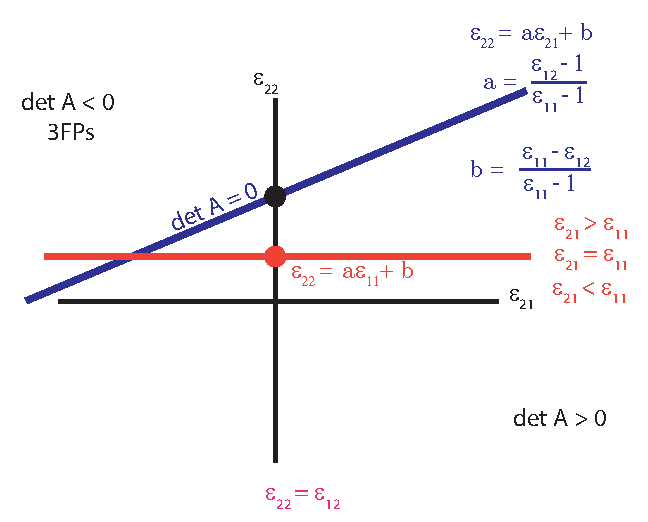
\includegraphics[width=\textwidth]{bla_parameter_space}
  \caption{A slice of the parameter space of the BLA for a fixed $\epsilon_{11}$ and $\epsilon_{12}$. %The different bifurcations can be found 
  }
  \label{fig:blaparameterspace}
\end{figure}


\subsubsection{Probability of bifurcation types}
We check what proportion of the bifurcation parameter space is constituted with bifurcations of the type that result in three fixed points.

The conditions are 
\begin{align*}
0 &< \epsilon_{11}\epsilon_{22}-\epsilon_{11}-\epsilon_{22}-\epsilon_{12}\epsilon_{21}-\epsilon_{12}-\epsilon_{21},\\
\epsilon_{22} &\leq \epsilon_{12},\\
\epsilon_{11} &\leq \epsilon_{21}.
\end{align*}


Because
\begin{align*}
\epsilon_{22} &\leq \epsilon_{12},\\
\epsilon_{11} &\leq \epsilon_{21}.
\end{align*}
we always have that
\begin{align*}
0 &< \epsilon_{11}\epsilon_{22}-\epsilon_{11}-\epsilon_{22}-\epsilon_{12}\epsilon_{21}-\epsilon_{12}-\epsilon_{21}.
\end{align*}


This implies that this bifurcation happens with $\frac{1}{4}$ probability in a $\epsilon$-ball around the BLA neural integrator with $\epsilon<1$.


\subsection{Fast-slow form}\label{sec:supp:fast_slow_form}

We transform the state space so that the line attractor aligns with the $y$-axis.
So, we apply the affine transformation $R_\theta(x-\frac{1}{2})$ with the rotation matrix $R_\theta = \begin{bmatrix}\cos\theta &-\sin\theta\\\sin\theta&\cos\theta\end{bmatrix}= \frac{1}{\sqrt{2}}\begin{bmatrix}1 &1\\-1&1\end{bmatrix}$ where we have set $\theta=-\frac{\pi}{4}$.
So we perform the transformation $x\rightarrow x'= R_\theta(x-\frac{1}{2})$ and so we have $x=R^{-1}_\theta x'+\frac{1}{2}$ with $R^{-1}_\theta = R_{-\theta}$.
Then we get that 
\begin{align}
R_{\theta}^{-1}\dot x' = \operatorname{ReLU}\left(W(R^{-1}_\theta x'+\frac{1}{2})+1\right)-R^{-1}_\theta x'-\frac{1}{2}.
\end{align}
For a perturbed connection matrix $W=\begin{bmatrix}\epsilon &-1\\-1&0\end{bmatrix}$ we get 
\begin{align}
R_{\theta}^{-1}\dot x' &= \operatorname{ReLU}\left(\frac{1}{\sqrt{2}}\begin{bmatrix}\epsilon &-1\\-1&0\end{bmatrix}\left(\begin{bmatrix}1 &-1\\1&1\end{bmatrix} x'+\frac{1}{2}\right)+1\right)-\frac{1}{\sqrt{2}}\begin{bmatrix}1 &-1\\1&1\end{bmatrix} x'-\frac{1}{2}\\
\dot x' &=\begin{bmatrix}-1 &1\\1&1\end{bmatrix}\left(\frac{1}{2}\begin{bmatrix}\epsilon-1 &-\epsilon-1\\-1&1\end{bmatrix}x' + \frac{1}{2\sqrt{2}}\begin{bmatrix}\epsilon-1 \\-1\end{bmatrix}+\begin{bmatrix}1 \\1\end{bmatrix}-\frac{1}{2}\begin{bmatrix}1 \\1\end{bmatrix}\right)-x'\\
\dot x' &=\left(\begin{bmatrix}-2 &0\\0&0\end{bmatrix}+\frac{\epsilon}{2}\begin{bmatrix}1 &-1\\-1&1\end{bmatrix}\right)x' + \frac{1}{2\sqrt{2}}\begin{bmatrix}\epsilon \\-\epsilon\end{bmatrix}
\end{align}

\section{Smoother activation functions}
It is well-known that activation functions ($\sigma$ in  Eqs.~\ref{eq:RNN:discrete} and  \ref{eq:RNN:continuous}), which can take many forms, play a critical role in propagating gradients effectively through the network and backwards in time \citep{jagtap2023,ramachandran2017,hayou2019}.
Activation functions that are $C^r$ for $r\geq 1$ are the ones to which the Persistence Theorem applies. 
The Persistence Theorem further specifies how the smoothness of the activation can have implications on the smoothness of the persistent invariant manifold.
For situations where smoothness of the persistent invariant manifold is of importance, smoother activation functions might be preferable, such as the Exponential Linear Unit (ELU)\citep{clevert2015} or the Continuously Differentiable Exponential Linear Units (CELU) \citep{barron2017}.








%%%%%%%%%%%%%%%%%%%%%%%%%%%%%%%%%%%%%%%%%%%%%%%%%%%%%%%%%%%%%%%%%%%%%%%%%%
%noisy learning with irnn, ubla and bla

%\subsection{Linear temporal integration task}\label{sec:task:continuous-clicks}
%Given a sequence of scalar input, the job of the network is to accumulate the values over time and report the final value at a later time.
%In the context of perceptual decision-making, subjects can be trained to perform the Poisson clicks task where they have to count the differing number of sensory stimulus events from the left and right side and report the side~\cite{brunton2013}.
%A linear integrator as a continuous attractor is a natural solution to such a task.
%We generalize the clicks to have associated continuous-values for the training of RNNs to discourage discrete counting solutions.
%
%We used discrete time representations over $T$ time bins and the stimulus encoded as difference of two non-negative values:
%\begin{align}
%    I_{t,i} &= m_{t,i} \cdot u_{t,i} 
%             \qquad & t=1,\dots, T, \ i=1,2 &&\text{(continuous clicks)}	\label{eq:input}
%    \\
%    O^\ast_{t} &= \sum_{s=0}^{t} \left(
%        I_{s,1} - I_{s,2}
%        \right)
%            \qquad  & t=1,\dots, T &&  \text{(desired output)} 			\label{eq:output}
%\end{align}
%where $m_{t,i}$ are independent Bernoulli random variables with probability $0.2$ and $u_{t,i}$ are independent random variables with uniform distribution on the unit interval.
%We used mean squared error (MSE) of the 1-dimensional output over time as the loss function over all time bins.
%We used $T=100$ time bins per trial unless specified otherwise.
%The gradients were computed in batch mode with $1024$ randomly generated trials.
%% The main challenges of this task are (1) addition and subtraction and (2) maintain the accumulated clicks for an extended period of time.
%
%% We designed a simple integration task where one of the optimal solutions is the continuous attractor. % <== not necessarily true!
%
%%The inputs for the clicks task are incoming clicks in two channels ($K=2$) and are given as follows.
%%The non-zero inputs follow a Poisson distribution with given rates.
%%At such time points, an input is sampled from $[0,1]$.
%%The task is to output the difference between the two inputs in the two channels. 
%
%%A noisy version of the task also includes noise added to a part of the input, without alternation to the target output, i.e., the noise added to the system should be ignored by the system.
%
%\subsubsection{RNN solutions to the linear integration task}\label{sec:rnn:integration}
%We use vanilla RNN implementations with the standard parameterization:
%%An RNN \citep{elmanFindingStructureTime1990} consists of a $N \times N$ transition matrix $W$, an $L \times N$ decoder matrix $\wout$ (where $L$ is the output dimension), a $N \times K$ encoder matrix $\win$ (where $K$ is the input dimension), and a bias $b$ for the hidden state and $\bout$ for the output.
%% If either the output or input is categorical, $M$ (respectively $N$) is the number of classes, and we use a one-hot representation. 
%%As the RNN ingests a sequence, at each timestep it updates to a hidden state $h$, and using the hidden state and the decoder matrix, produces outputs $y$:
%\begin{equation}
%  \begin{aligned}
%	\vx_t &= \sigma(\win \vI_t + \vW \vx_{t-1} + \vb) \label{eq:RNN:discrete}\\
%	O_t &= \wout \vx_t + \bout
%  \end{aligned}
%\end{equation}
%where $\vx_t \in \reals^d$ is the hidden state, $\vI_t \in \reals^K$ is the input,
%$\sigma: \reals \to \reals$ an activation function which acts on each of the hidden dimension, and
%$\vW, \vb, \win, \wout, \bout$ are parameters.
%Assuming an Euler integration with unit time step, the discrete-time RNN of \eqref{eq:RNN:discrete} corresponds to the ODE:
%\begin{align}
%    \dot{\vx} &= -\vx + \sigma(\win \vI + \vW \vx + \vb). \label{eq:RNN:continuous}
%\end{align}
%%
%For tractable analysis, we consider $2$ dimensional systems with ReLU activation. %We include another continuous attractor, the identity RNN, which is also a popular initialization for RNN training \citep{le2015}.
%We study the three different ReLU RNN implementations of a perfect integrator in a 2 dimensional system, the Identity RNN (iRNN), UBLA and BLA (we refer to the line attractors together as LA).
%These three networks have same norm in the recurrent matrix $\vW$ but not close in the parameter space.
%On the original clicks task the UBLA and BLA networks count the click differences directly, while iRNN counts the clicks separately and then subtracts these representations through the output mapping.
%The behaviors of UBLA and BLA in the absence of stimulus are shown in Fig.~\ref{fig:ublabla}, while the behavior of the iRNN is trivial since there is no flow. These networks are defined as follows.
%
%\paragraph{Identity RNN~\citep{le2015}}
%\label{sec:ubpa,sec:iRNN}
%%This is an RNN with the identity matrix as its recurrent weights  with two hidden units. 
%\begin{equation}\label{eq:irnn}
%\win = 
%\begin{pmatrix}
%1  &  0 \\
%0 &  1
%\end{pmatrix}, \
%\vW = 
%\begin{pmatrix}
%1  &  0 \\
%0  &  1
%\end{pmatrix}, \
%\wout = 
%\begin{pmatrix}
%-1  \\  1 
%\end{pmatrix}, \
%\vb = 
%\begin{pmatrix}
%0  \\ 0
%\end{pmatrix}, \
%\bout = 0.
%\end{equation}
%
%%The system has the whole state space as its invariant manifold.
%
%\paragraph{Unbounded line attractor}
%We formulate this implementation of a bounded integrator with a parameter that determines step size along line attractor $\alpha$. Together with the parameters for the output bias $\beta$ the parameters determine the capacity of the network. While the line attractor is unbounded from above, it only extends to the center from below.  The step size along line attractor $\alpha$ determines the maximum number of clicks as the difference between the two channels; the capacity is $\beta/\alpha$ number of clicks.
%\label{sec:ubla}
%\begin{equation}\label{eq:ubla}
%\win = \alpha
%\begin{pmatrix}
%-1  &  1 \\
%-1  &  1
%\end{pmatrix}, \
%\vW = 
%\begin{pmatrix}
%0  &  1 \\
%1  &  0
%\end{pmatrix}, \
%\wout = \frac{1}{2\alpha}
%\begin{pmatrix}
%1  \\  1 
%\end{pmatrix}, \
%\vb = 
%\begin{pmatrix}
%0  \\  0
%\end{pmatrix}, \
%\bout = -\frac{\beta}{\alpha}.
%\end{equation}

%\subsubsection{Asymmetric loss landscape reflecting dynamics after bifurcation}\label{sec:asymmetricloss}
%To illustrate the effect of bifurcations from the continuous attractor solution, we take a 1-dimensional slice of the loss surface, see Fig.~\ref{fig:maintenance_h0}B.
%Specifically, we continuously vary one of the entries of the self-recurrent connection matrix: $    \vW_{1,1} \leftarrow \vW_{1,1} + \Delta$. % with $\Delta\in[-\tfrac{1}{10},\tfrac{1}{10}].$
%At any $\Delta \neq 0$, the continuous attractor disappears and the spontaneous dynamics of the networks show convergent and/or divergent behavior at exponential rates.
%Therefore, as the number of time steps in a trial increases, the error in the output also exponentially converge or diverge in a corresponding manner.
%As can be seen in Fig.~\ref{fig:maintenance_h0}B, for UBLA and iRNN, $\Delta > 0$  perturbations shows exponentially increasing loss and corresponds to an exploding gradient dynamical system.
%In all other cases, including all perturbations of BLA, leads to vanishing gradient, hence the loss is bounded.
%Note also the high curvature of the loss landscape around the optimal solution indicating that the slow manifold may only be maintained in a small neighborhood around the optimal solution, especially for the LAs.

%
%\subsubsection{Maintaining a neural integrator}\label{sec:exp:maintaining}
%The theory of persistent invariant manifolds for compact continuous attractors suggests that the BLA should have bounded gradients (unlike UBLA and iRNN) and hence it should be easier to maintain it in the presence of noise.
%To investigate the differential effect of stochastic gradient descent (SGD) on the three neural integrator models, we performed three learning experiments using the continuous-valued click integration task.
%The input and output are defined as in Eqs.~\ref{eq:input} and \ref{eq:output} with $I_{t,i}=0$ for $t=11,\dots,T$.
%%T=100,500,1000
%We investigate the effects of perturbations of the recurrent matrix on the learning of the parameters during gradient descent starting from the perfect solutions to the task.  Gradient step were taken with a fixed gradient step size $\lambda$ (learning rate).
%%MSE at last time step
%%For SGD, the output of the network over $T$ steps was taken to calculate the loss based on the mean squared error (MSE) over a batch of 1024 trials.
% We set $\alpha=1$ and $\beta=20$ in Eq \ref{eq:ubla} and \ref{eq:bla}. The hidden state at the start of a trial is a learnable parameter. 
%
%In the first experiment, Gaussian random noise is injected to all parameters inducing a constant diffusion of the parameters, which emulates the biological synaptic variability.
%This type of noise is directly applied to the weights as $ \vW \leftarrow \vW + \vV$ with $\vV_{i,j}\sim\mathcal{N}(0,\sigma)$. To dissociate the effect of misadjustment from gradient descent and external perturbation, we measured the effect of a single perturbation on the learning dynamics.
%Fig.~\ref{fig:maintenance_h0}C shows that for all networks, gradient descent (with constant learning rate, chosen from a grid search) was able to counter the diffusion.
%%The distribution of MSE for the task can be used as proxy for the misadjustment from the optimal solution.
%BLA and UBLA with learning have superior misadjustment compared to iRNN and compared to perturbations without learning, while the BLA has the broadest range of learning rates that are optimal and far away from exploding gradients (Fig.~\ref{fig:maintenance_h0}A).
%BLA has a slight advantage in terms of a smaller spread of MSE compared to UBLA.
%The invariant manifold of the BLA is persistent throughout learning in many cases, see \ref{sec:supp:learning} and Fig.~\ref{fig:vfs1}. However, the gradients are not pointing towards the BLA but to one of the bifurcations of the BLA (see Supp~Fig.~\ref{fig:wdn_mse_trajectories_F1}, Fig.~\ref{fig:vfs5} and Supp. Fig.~\ref{fig:vfs30}). We determine the alignment of the gradient as the cosine similarity of the gradient step with the vector in recurrent parameter space that points towards the initial parameters at every gradient step and use a cutoff of a maximum deviation of 45\textdegree\  as aligned gradients with the optimal solution direction.
%iRNN often finds a different optimum (it settles at a part of the state space that is at a non-zero distance from the initial recurrent matrix and bias (Fig.~\ref{fig:maintenance_h0}D and Fig~\ref{fig:vfs1}).
%UBLA can stay close to the initial solution for a small enough learning rate (Fig.~\ref{fig:maintenance_h0}D and E) and maintains a slower flow than the BLA (Fig.~\ref{fig:speeds}).
%
%
%%The noise level $\sigma$ was chosen individually for the three networks as follows. 
%We calculated the loss on a batch of inputs for various noise levels $\sigma$ for all three noise types (Fig.~\ref{fig:matching_noise_3types_cont}).
%We chose a matched noise level per integrator that corresponded to a set average loss averaged over 200 weight perturbations (see also in Sec.~\ref{sec:supp:matching}).
%This way of matching noise level to induce the same loss should be a universal approach to be able to compare the performance of different networks.
%
%%description of finding optimal learning rate
%For the matched noise level, we find the optimal learning rate for each network separately.
%The optimal learning rates for the input-type noise experiments were chosen from a set of values 
%($\{(1+j\frac{1}{4}))10^{-i}\}_{i=4,\dots 10, j=1,2,3}$))  based on best performance of the task, measured as mean MSE of the last ten epochs averaged over ten runs.
%The slow manifold that is created after perturbations provides gradients that can counteract parameter diffusions for all networks (on short trials), even for the ones that have the potential for exploding gradients (Fig.~\ref{fig:maintenance_h0}A and C).
% %new conclusions
%We use the normed difference to the initial parameters at every gradient step as proxy for the misadjustment from the optimal solution (Fig.~\ref{fig:maintenance_h0}D and E).
% We further show that all networks converge to a different (from the initialization), non-optimal, solution as they settle in a regime in parameter space that has a higher norm difference with the initial parameters of the neural integrator in ten different runs with the same random seed for the noise for the three integrators (Fig.~\ref{fig:maintenance_h0}D and E).
% We conclude therefore that, in practice, it is difficult to maintain any of the continuous attractors.
%
%%gradientdistribution 
%%Then we looked for networks that diverged due to exploding gradients which we identify as having a loss of 1 or higher. 
%Note that exploding gradients can be seen for UBLA manifested as the bimodal distribution of the gradients in Fig.~\ref{fig:maintenance_h0}F. This does lead to faster divergence (for lower learning rate) but has on the other hand the benefit of providing useful gradients to maintain the (local) solution around the optimal solution, which explains the superior performance at the optimal learning rate for the UBLA (Fig.~\ref{fig:maintenance_h0}A), on this timescale for the trial that we investigated.
%Also in the presence of input and internal noise the UBLA has a higher tendency to have exploding gradients for lower learning rates, see Fig.~\ref{fig:all_lrs_vs_mses}. 
%%This is because the noise sometimes pushes the UBLA to the regime with divergent dynamics which leads to exploding gradients, which then causes the weights to make bigger jumps.
%%The fact that the iRNN has a smaller range of gradients explains exploding gradients at a higher learning rate for iRNN and the need for a higher learning rate for optimal maintenance of the solution and is explained by a more shallow loss landscape in the close vininity of the iRNN (Fig.~\ref{fig:maintenance_h0}C).
%We hypothesise that the negative effect of exploding gradients shows only for longer trials.
%
%
%\begin{figure}[H]
%  \centering
%  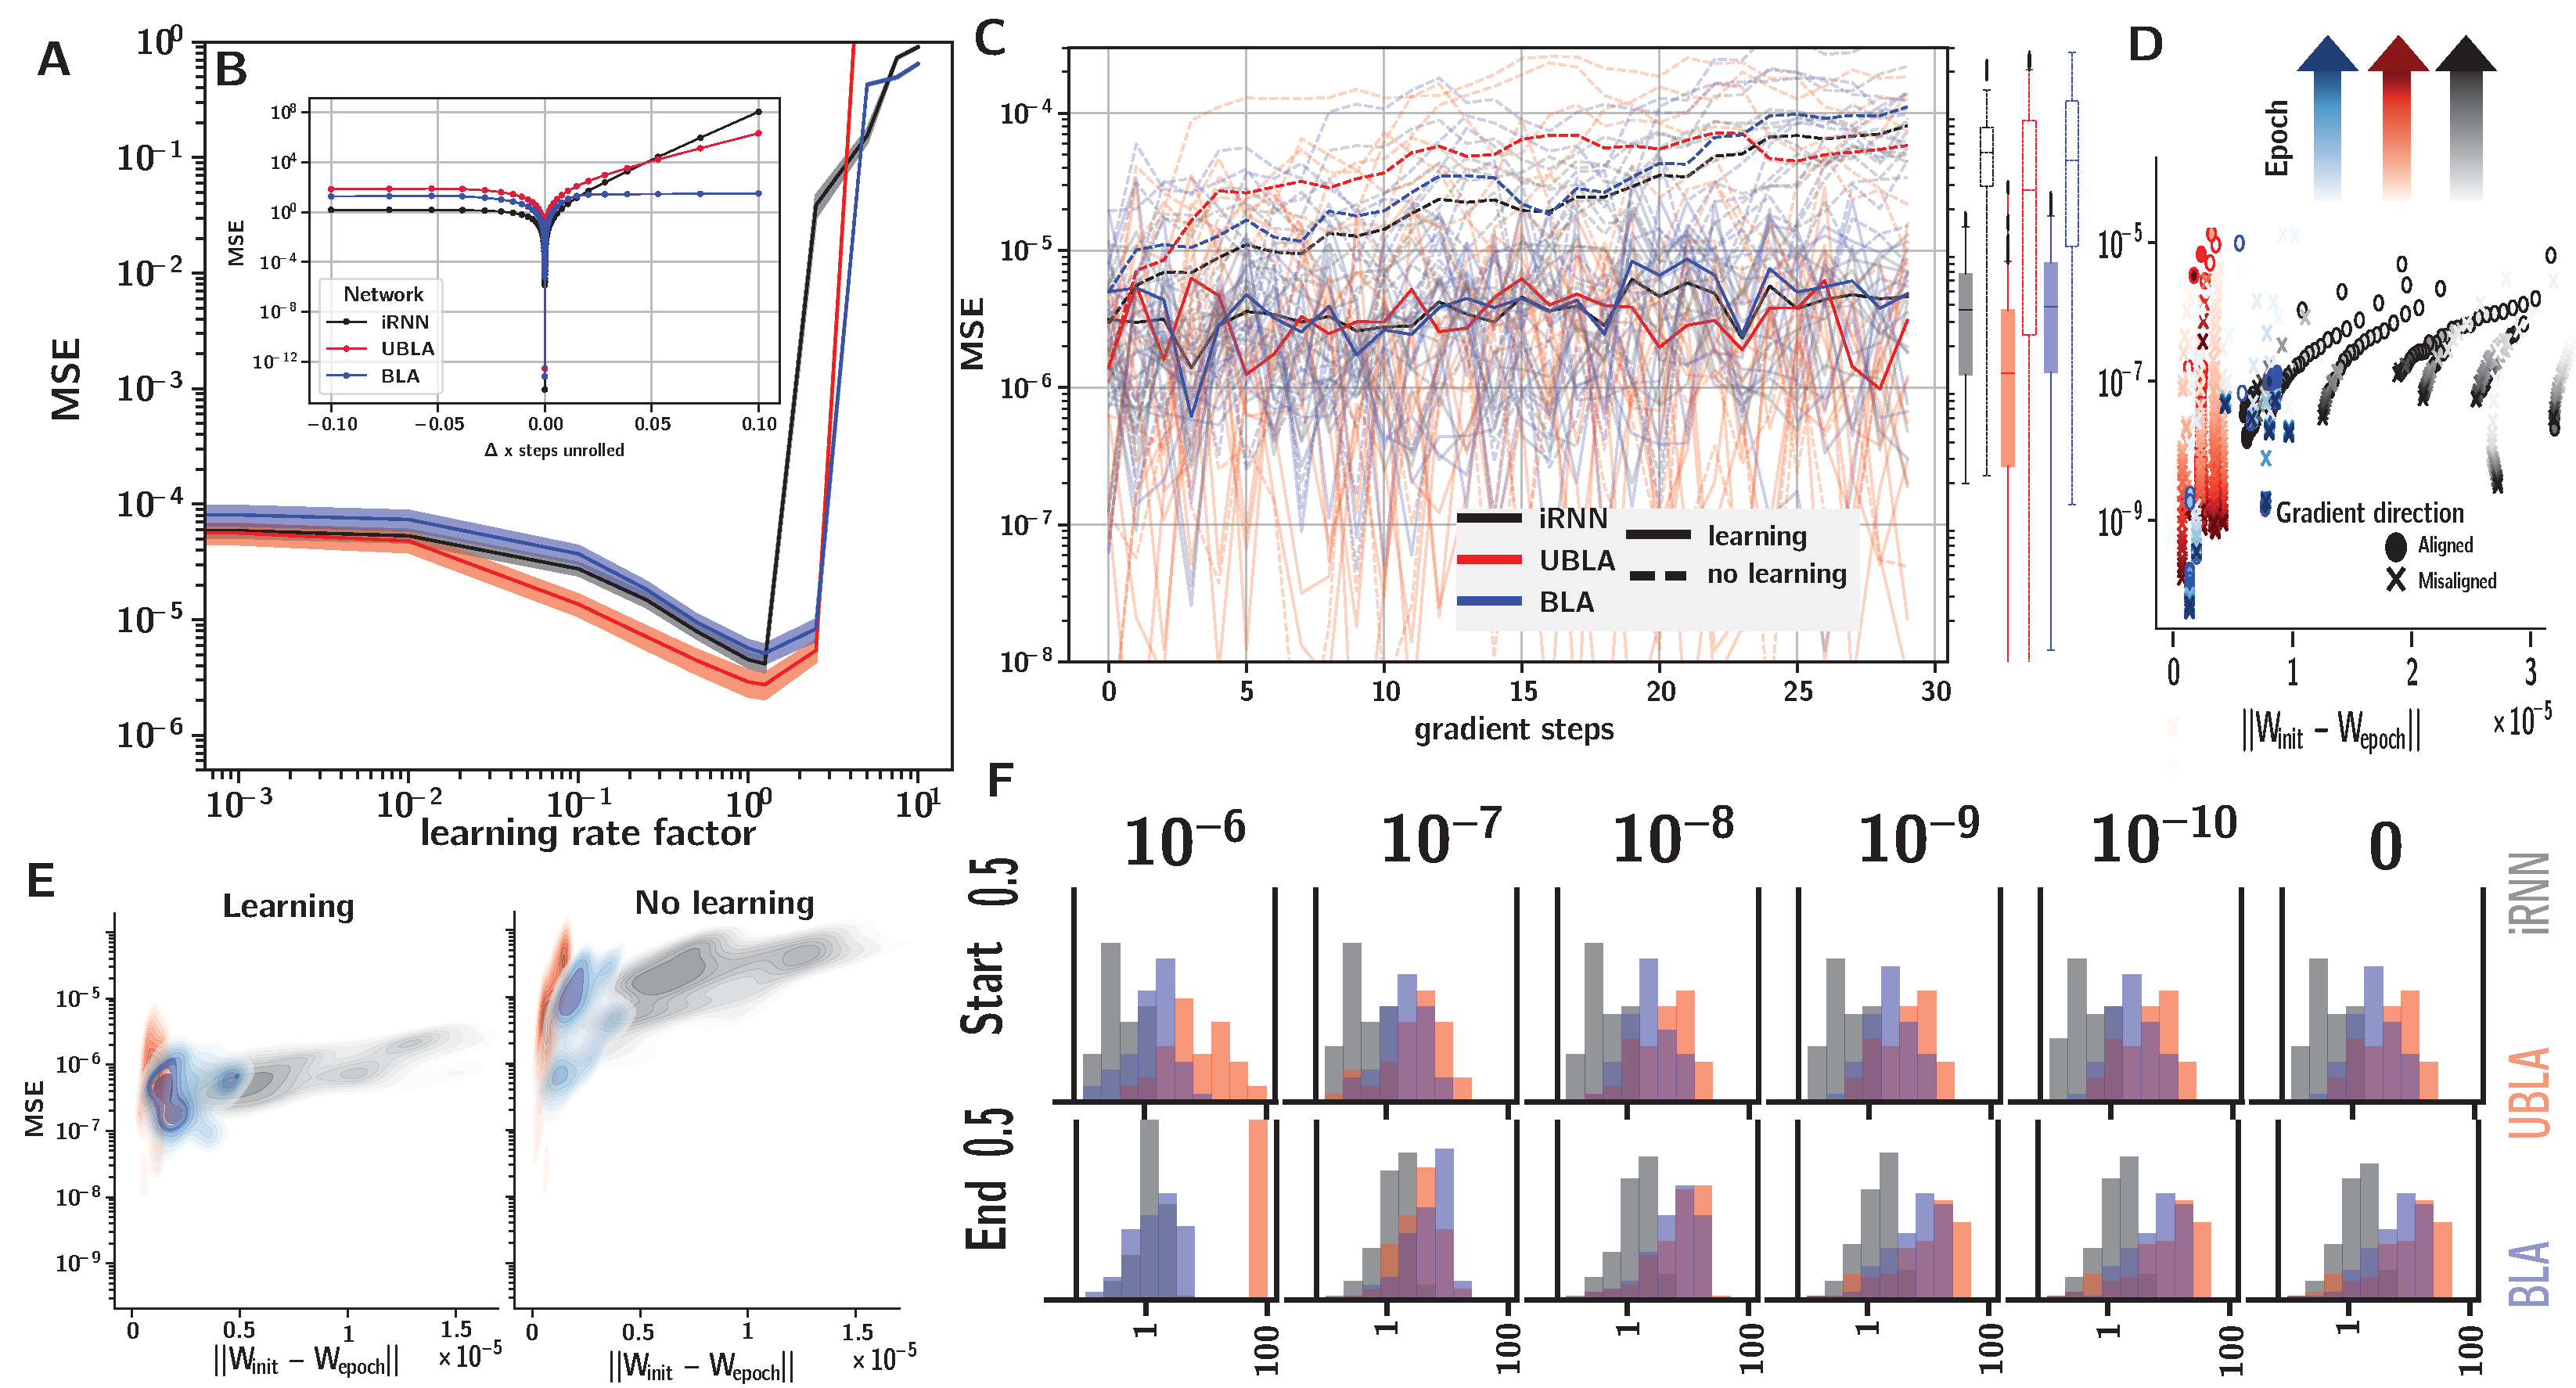
\includegraphics[width=\textwidth]{maintenance_h0_less}
%  \caption{
%  Comparing three continuous attractor solutions on the click integration task of $T=100$ time steps.
%(A) MSE distribution during learning with different learning rates.
%(B) Loss landscape is steeper around the attractors. The BLA has a bounded loss in its neighborhood.
%(C) MSE distribution during learning and in the presence of noise. Learning counteracts diffusion in all three-types of initializations.
%(D) All networks converge to local non-optimal solutions after a single perturbation in 30 gradient steps.
%(E) Distance of parameters to original during learning with noise (left) and without learning (right).
%(F) Gradient distribution at the beginning (upper) and end (lower) of trials.
%  }
%  \label{fig:maintenance_h0}
%\end{figure}


%\newpage
%\section{Internal and input noise and noise level matching}\label{sec:supp:matching}
%%Rationale: what is a universal measure of noise level
%%that is applicable to any dyn sys and makes comparisons of performance (under gradient descent) meaningful?
%
%
%We investigate the effects of two other types of noise on the learning of the parameters during gradient descent starting from the perfect solutions to the task.
%We investigated the effect of learning when perturbations are induced by the backpropagated gradient which is structured by the recurrent dynamics in the following two ways.
%The second type of noise is injected into the input $x_{i,t}+\epsilon_{i,t}$ with $\epsilon\sim\mathcal{N}(0,\sigma)$.
%To inject noisy gradients naturally, we added noise to the input to the first 10 time steps during the trial that were not integrated in the target output $O_t^*$ (Eq.~\ref{eq:output}).
%The third type of noise is injected into the hidden state $h_{i,t}+\epsilon_{i,t}$ with $\epsilon\sim\mathcal{N}(0,\sigma)$ for $t=1,\dots, T$ and $i=1,2$. 
%
%\begin{figure}[thbp]
%     \centering
%    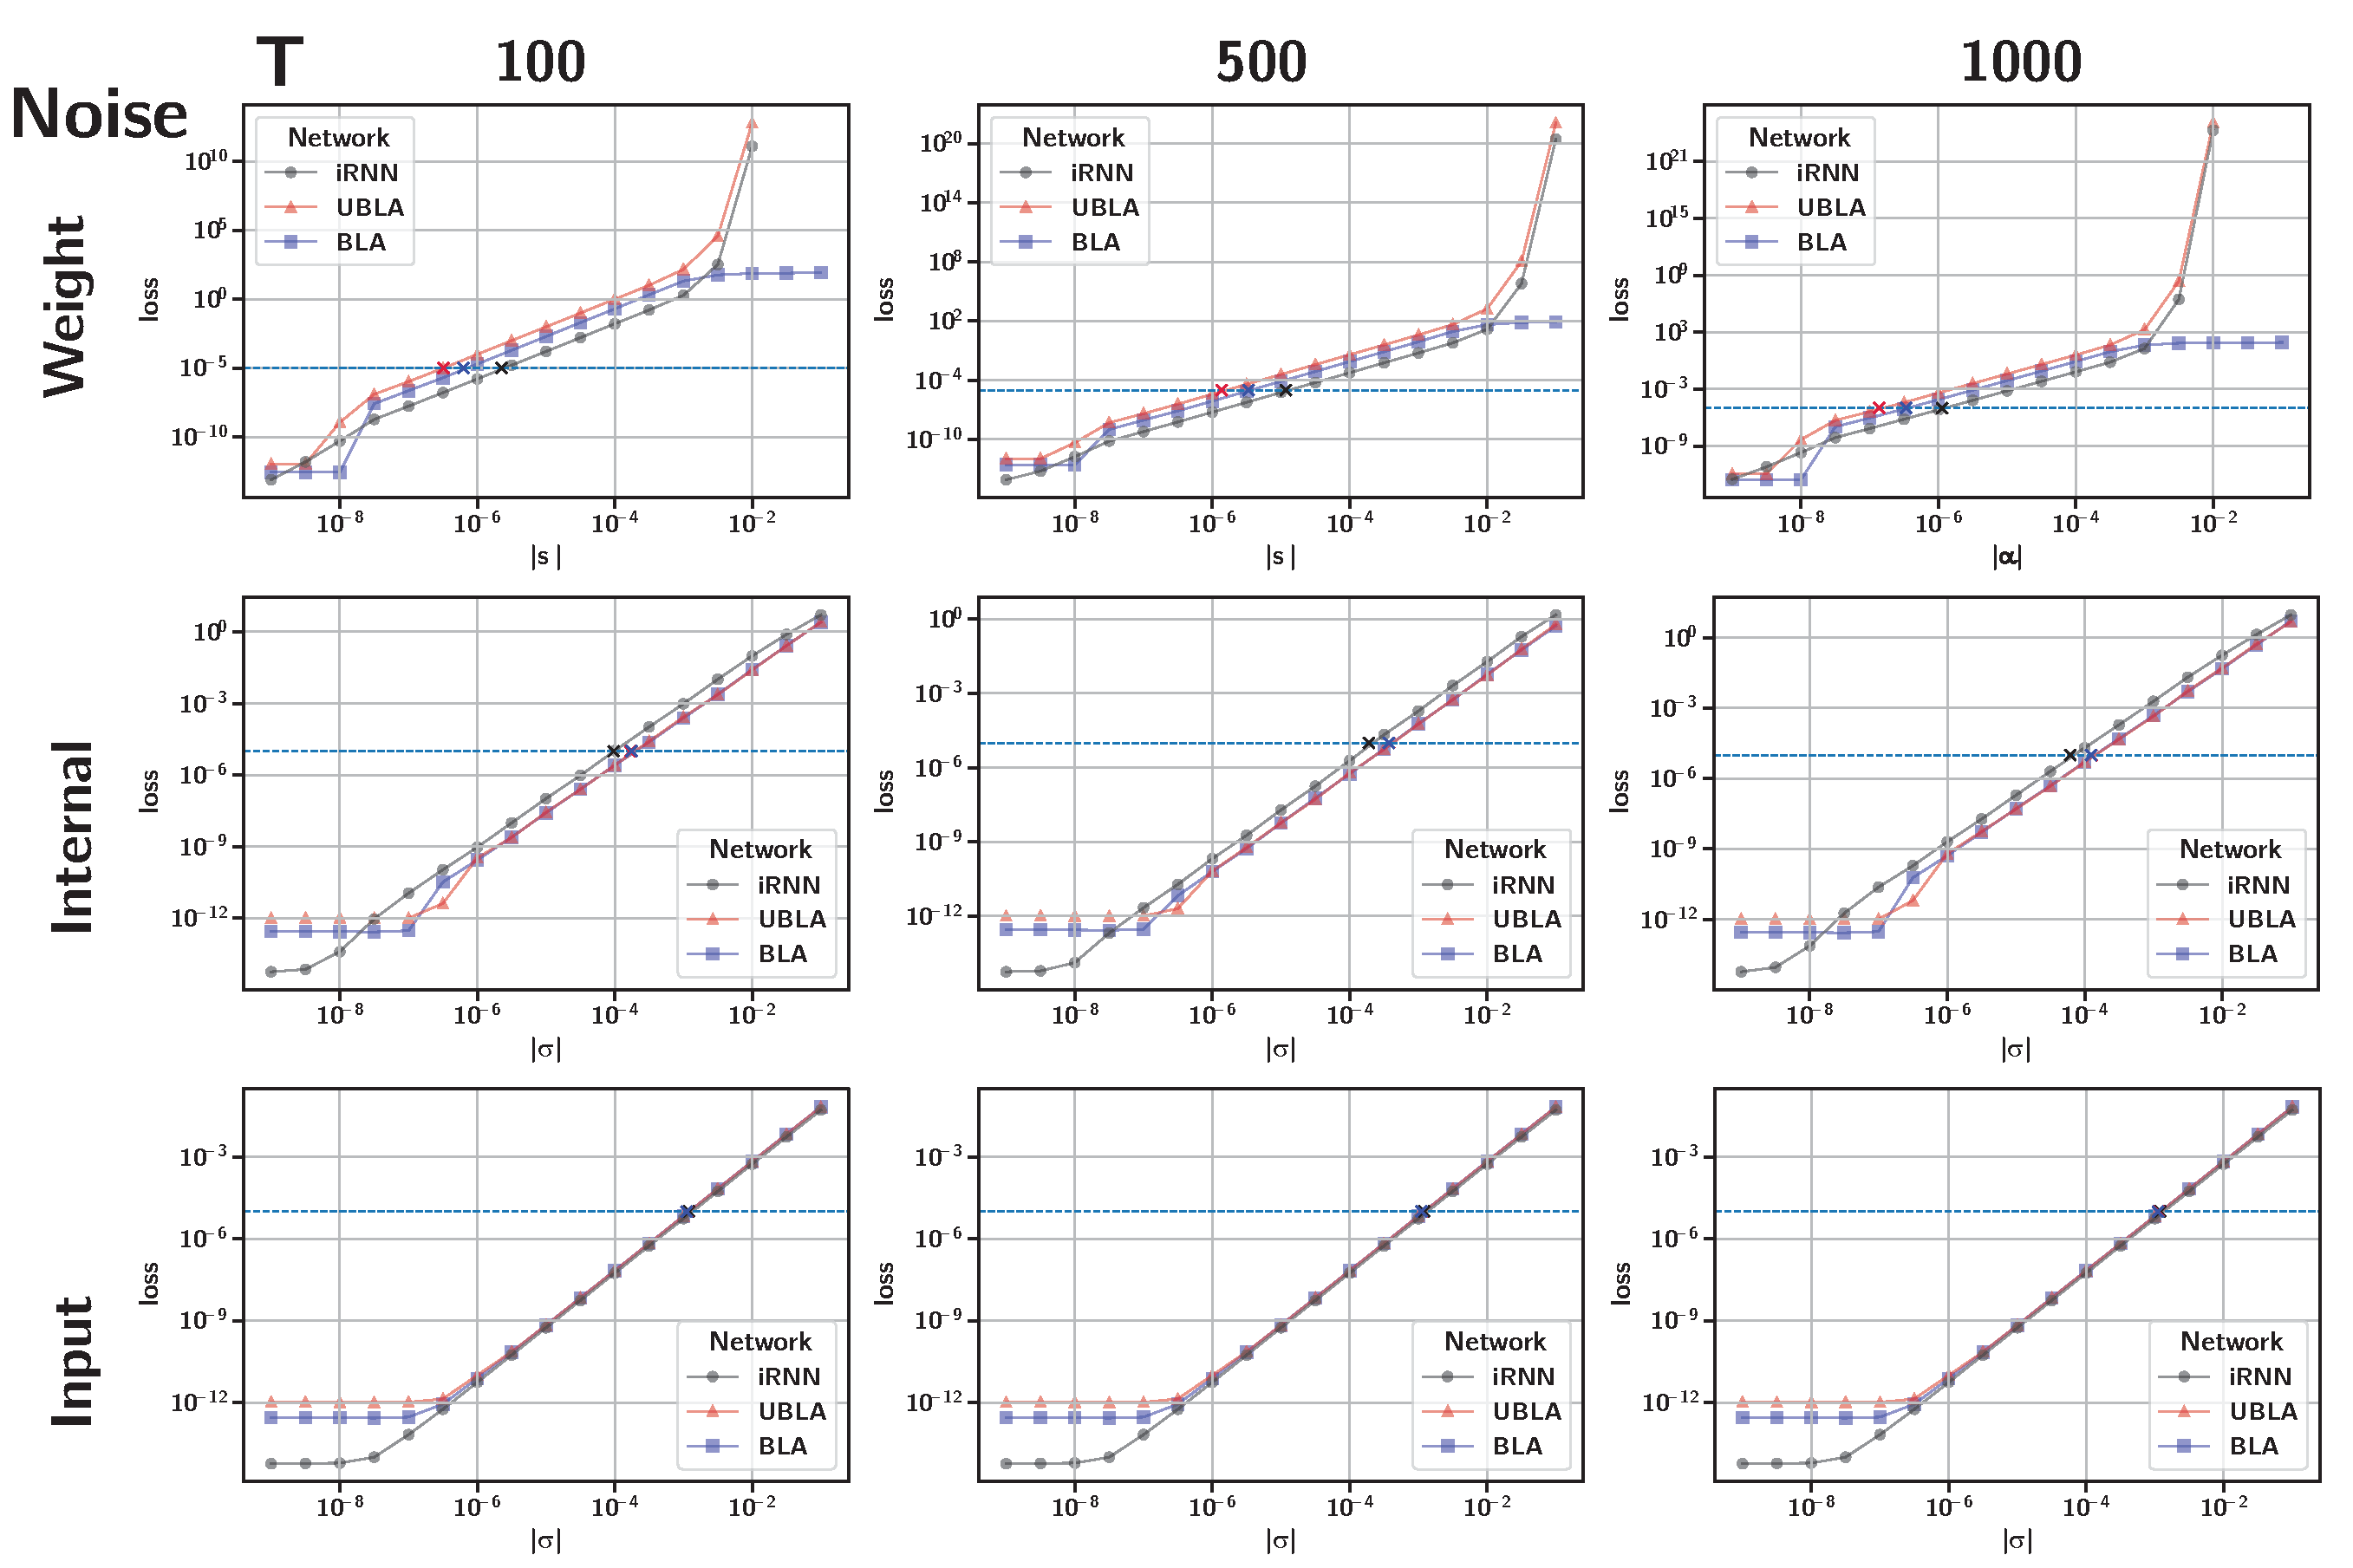
\includegraphics[width=\textwidth]{matching_noise_3types_cont}
%       \caption{For various values the loss was calculated for the three types of noise. The matched noise levels were chosen based on these curves.}
%         \label{fig:matching_noise_3types_cont}
%\end{figure}
%
%\newpage
%\section{Continuous attractor solutions in click integration tasks with noise in the weights}
%For the SGD, the last output of the network after $T$ steps was taken to calculate the loss based on the mean squared error (MSE) over a batch of 1024 trials. 
%
%\begin{figure}[thbp]
%  \centering
%  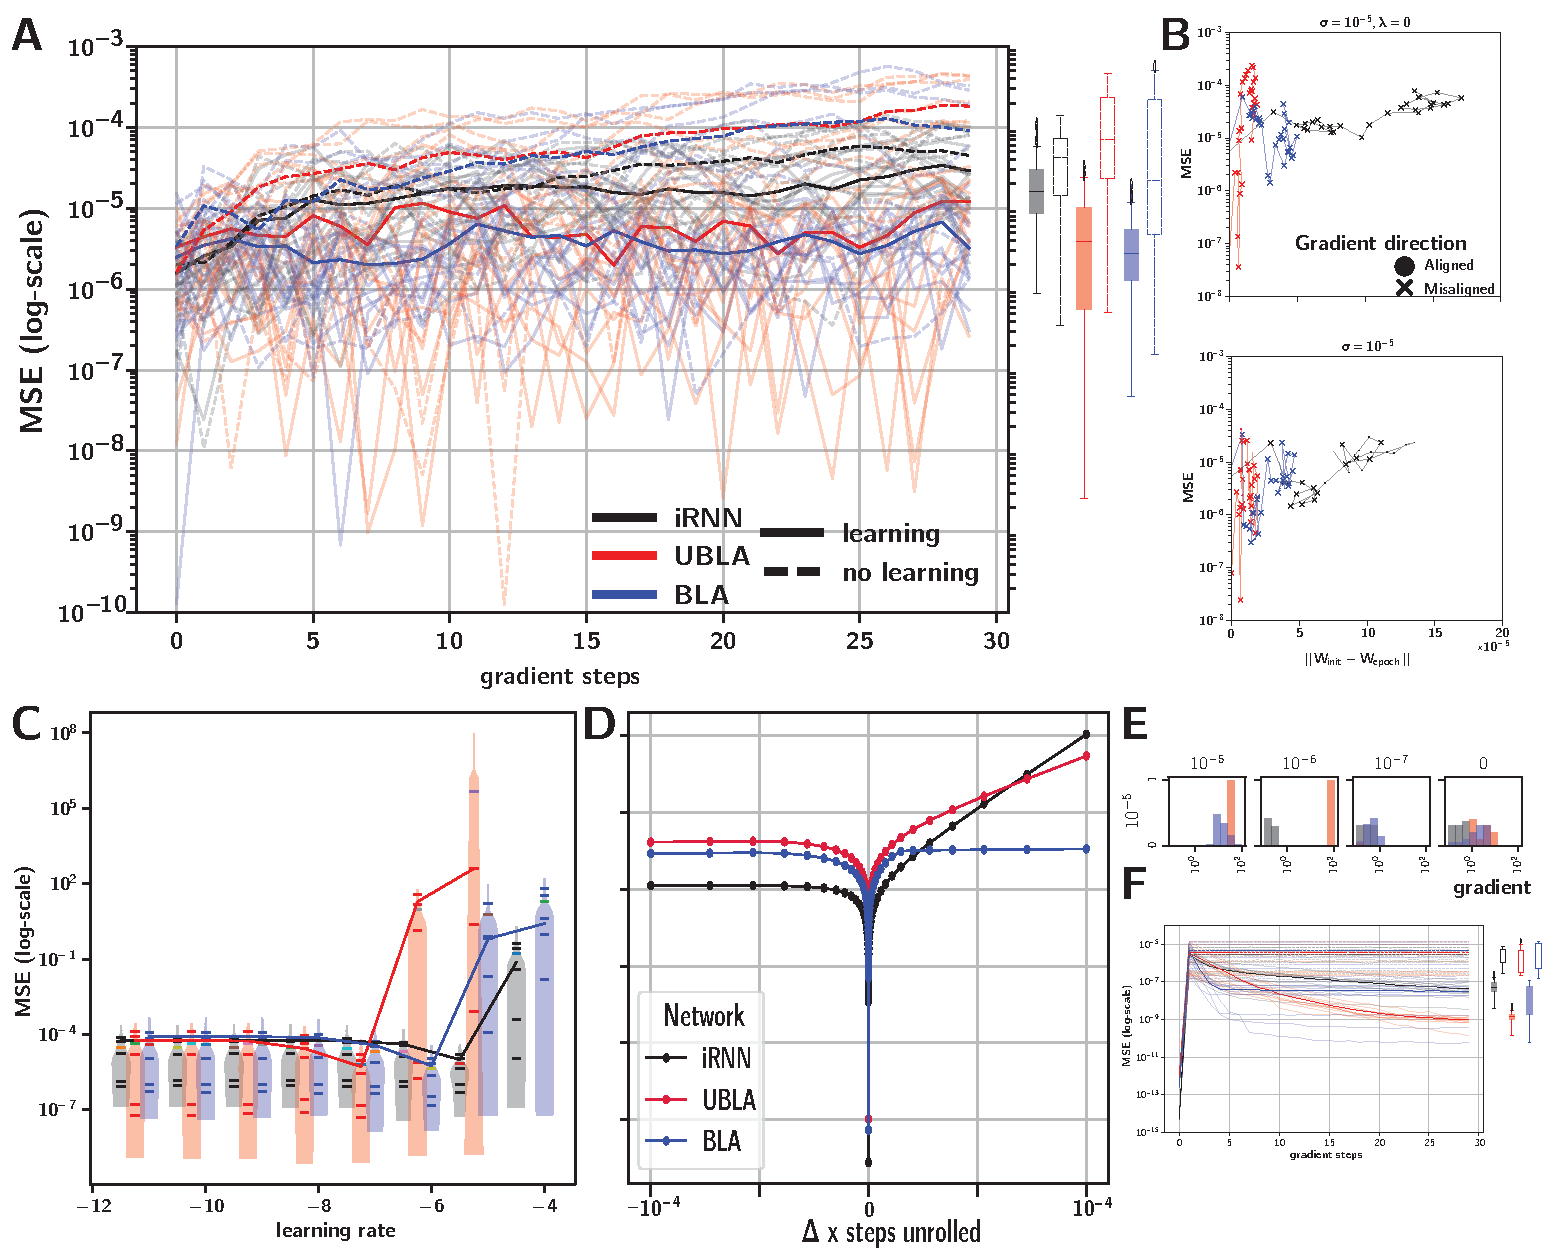
\includegraphics[width=\textwidth]{maintenance_T100}
%  \caption{
%  Comparing three continuous attractor solutions to the click integration task for a length of $T=100$ time steps.
%  (A) Effect of gradient descent in repairing the continuous attractor. RNNs without gradient descent (dashed line) are shown for reference. Box plots show distribution of the loss for the last 10 steps. Averages (thick lines) over 10 simulations (thin lines) are shown for each network.
%  (B) Changes to the recurrent parameters (matrix and bias), without (upper) and with (lower) learning (with the optimal learning rates). iRNN converges to a different solution.
% (C)  The distribution of the MSE for different learning rates. The dip in the MSE defines the optimal learning rate for each of the three neural integrators. 
%    (D) Single parameter perturbation showing exploding gradients for iRNN and UBLA.
%  (E) Distribution of gradients shows bimodal distribution for UBLA. %Gradient distributions for all noise levels and learning rates. For some noise levels a bimodal distribution can be seen for the LAs, but exploding gradients seem to be absent for iRNN for low learning rates.
%    (F) Interleaved weight perturbations showing quick recovery for BLA and and slow for iRNN and UBLA.
%  }
%  \label{fig:maintenance}
%\end{figure}
%
%\begin{figure}[thbp]
%  \centering
%  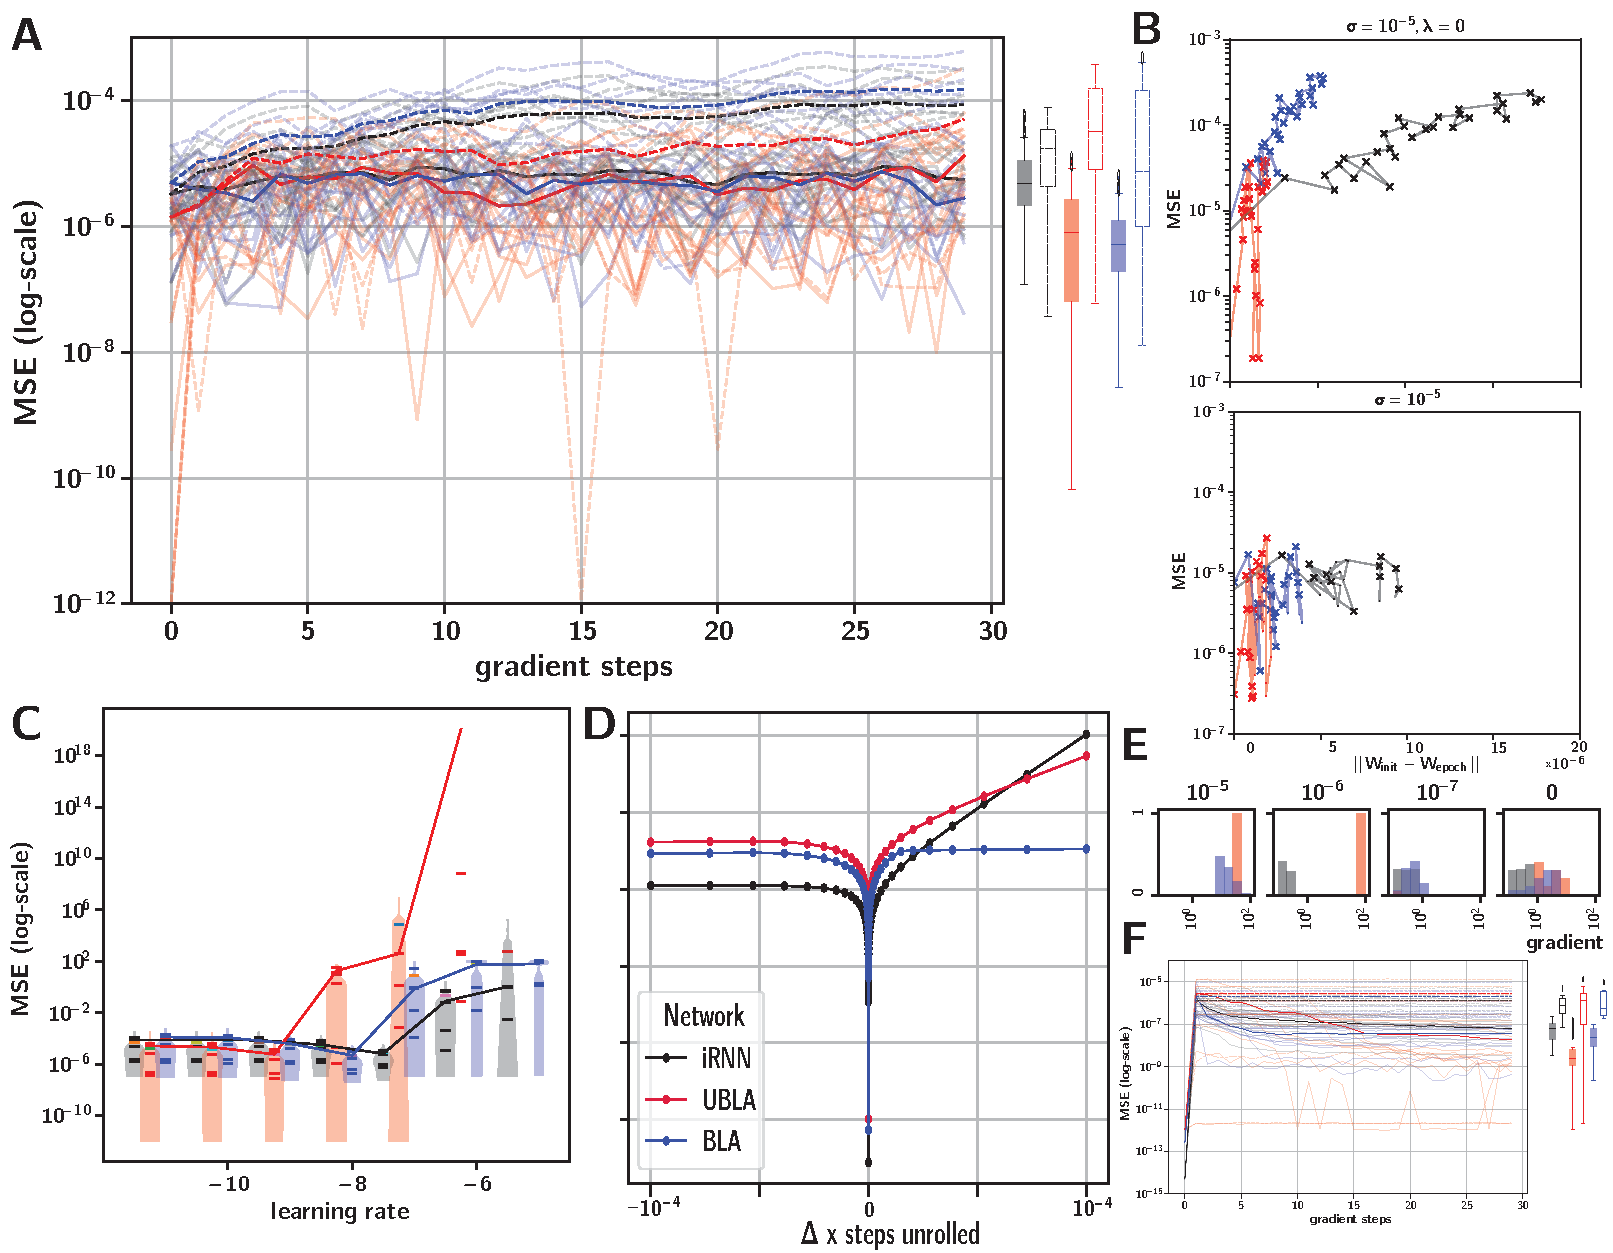
\includegraphics[width=\textwidth]{maintenance_T1000}
%  \caption{
%  Comparing three continuous attractor solutions to the click integration task for a length of $T=1000$ time steps.
%  (A) Effect of gradient descent in repairing the continuous attractor. RNNs without gradient descent (dashed line) are shown for reference. Box plots show distribution of the loss for the last 10 steps.
%  (B) Changes to the recurrent parameters (matrix and bias), without (upper) and with (lower) learning (with the optimal learning rates). iRNN converges to a different solution.
% (C)  The distribution of the MSE for different learning rates. The dip in the MSE defines the optimal learning rate for each of the three neural integrators. 
%    (D) Single parameter perturbation showing exploding gradients for iRNN and UBLA.
%  (E) Distribution of gradients shows bimodal distribution for UBLA.
%    (F) Interleaved weight perturbations showing quick recovery for BLA and and slow for iRNN and UBLA.
%  }
%  \label{fig:maintenance:long}
%\end{figure}
%
%\newpage
%\section{Stability of the neural integrators for different learning rates}
%
%\begin{figure}[thbp]
%     \centering
%    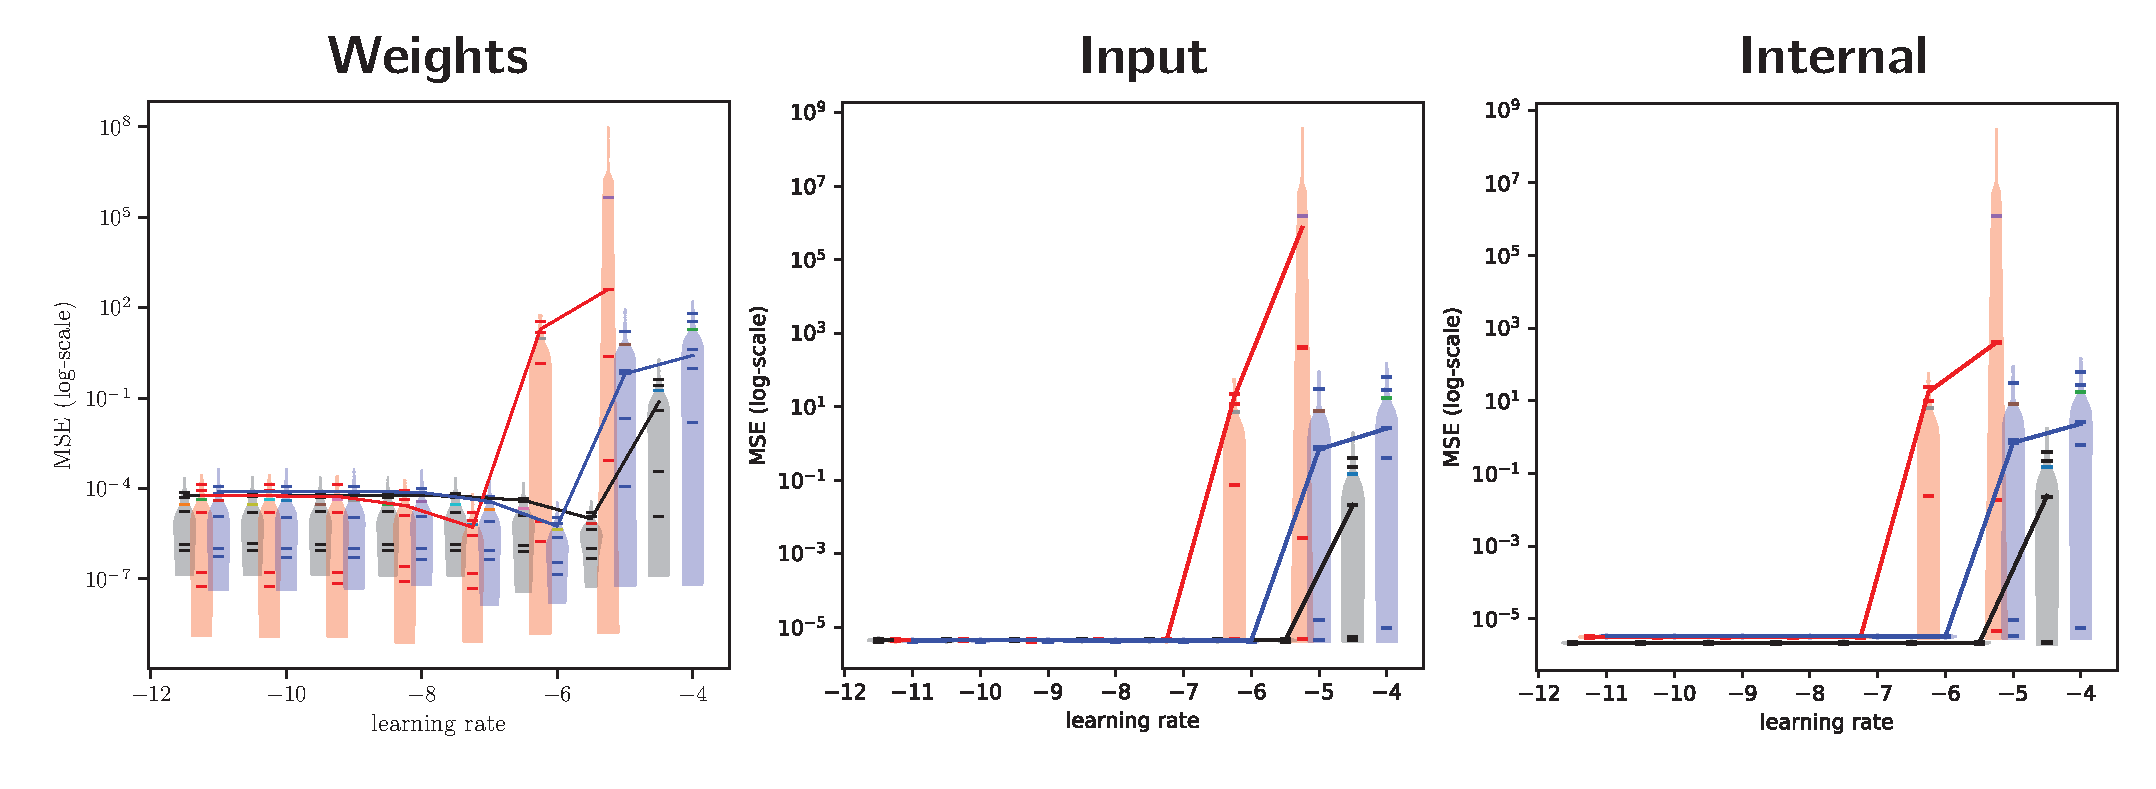
\includegraphics[width=\textwidth]{all_lrs_vs_mses_f1}
%       \caption{Distribution of MSE for the three noisy types for different learning rates.}
%         \label{fig:all_lrs_vs_mses}
%\end{figure}
%
%
%\newpage
%\section{Trajectories of the neural integrators in the recurrent network space}
%
%\begin{figure}[thbp]
%     \centering
%    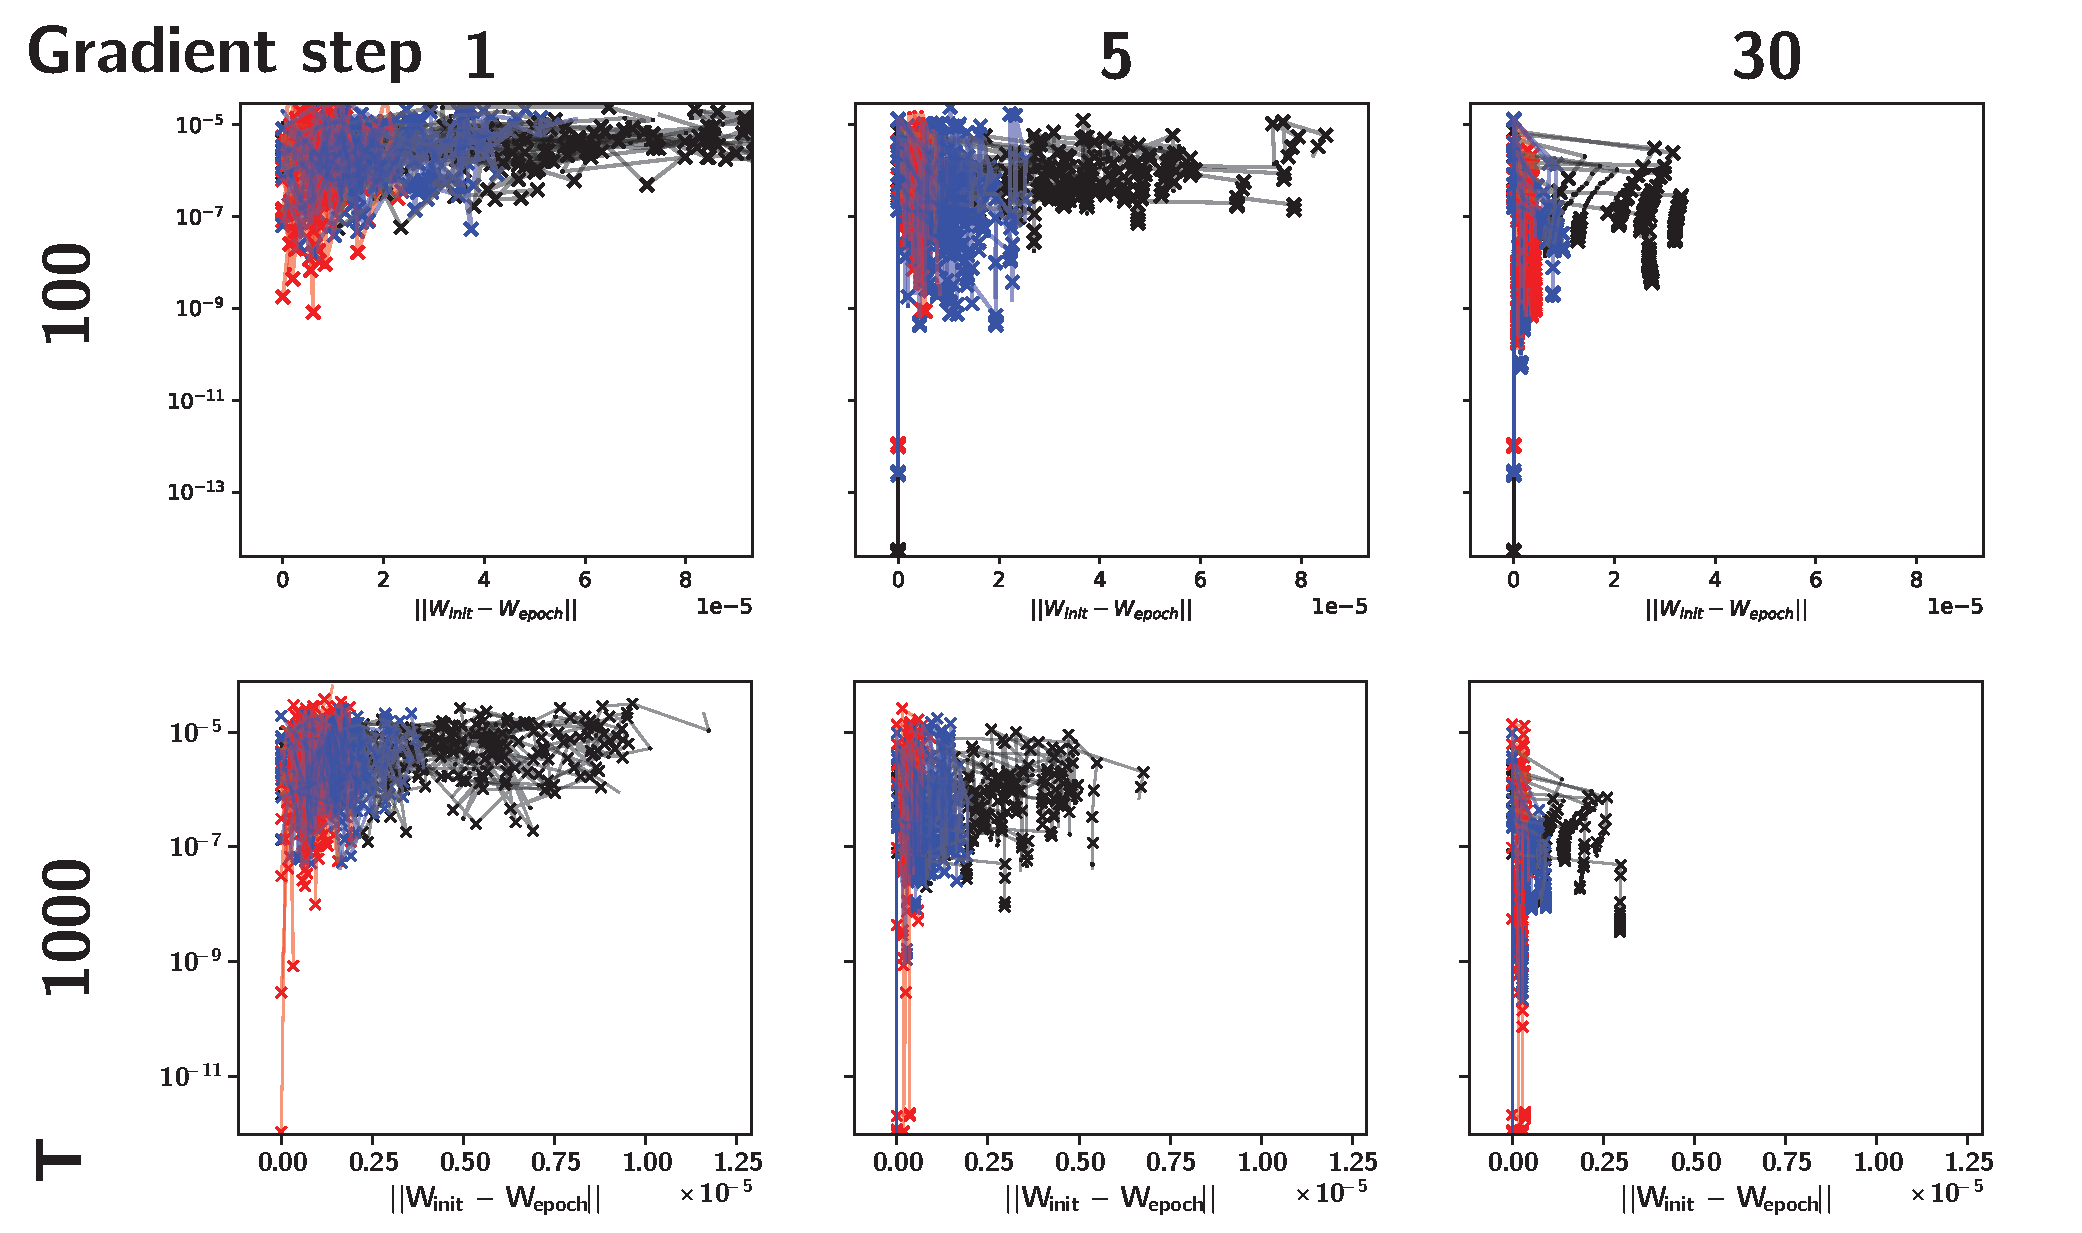
\includegraphics[width=\textwidth]{wdn_mse_trajectories_F1}
%       \caption{Trajectories of learning in parameter space relative to the initial recurrent parameters. The LAs follow a trajectory that is orthogonal to the initial parameters, but that yet decreases the MSE.}
%         \label{fig:wdn_mse_trajectories_F1}
%\end{figure}
%
%
%\newpage
%\section{Influence of the different noise types on the found solutions for the neural integrators}
%
%\begin{figure}[H]
%     \centering
%    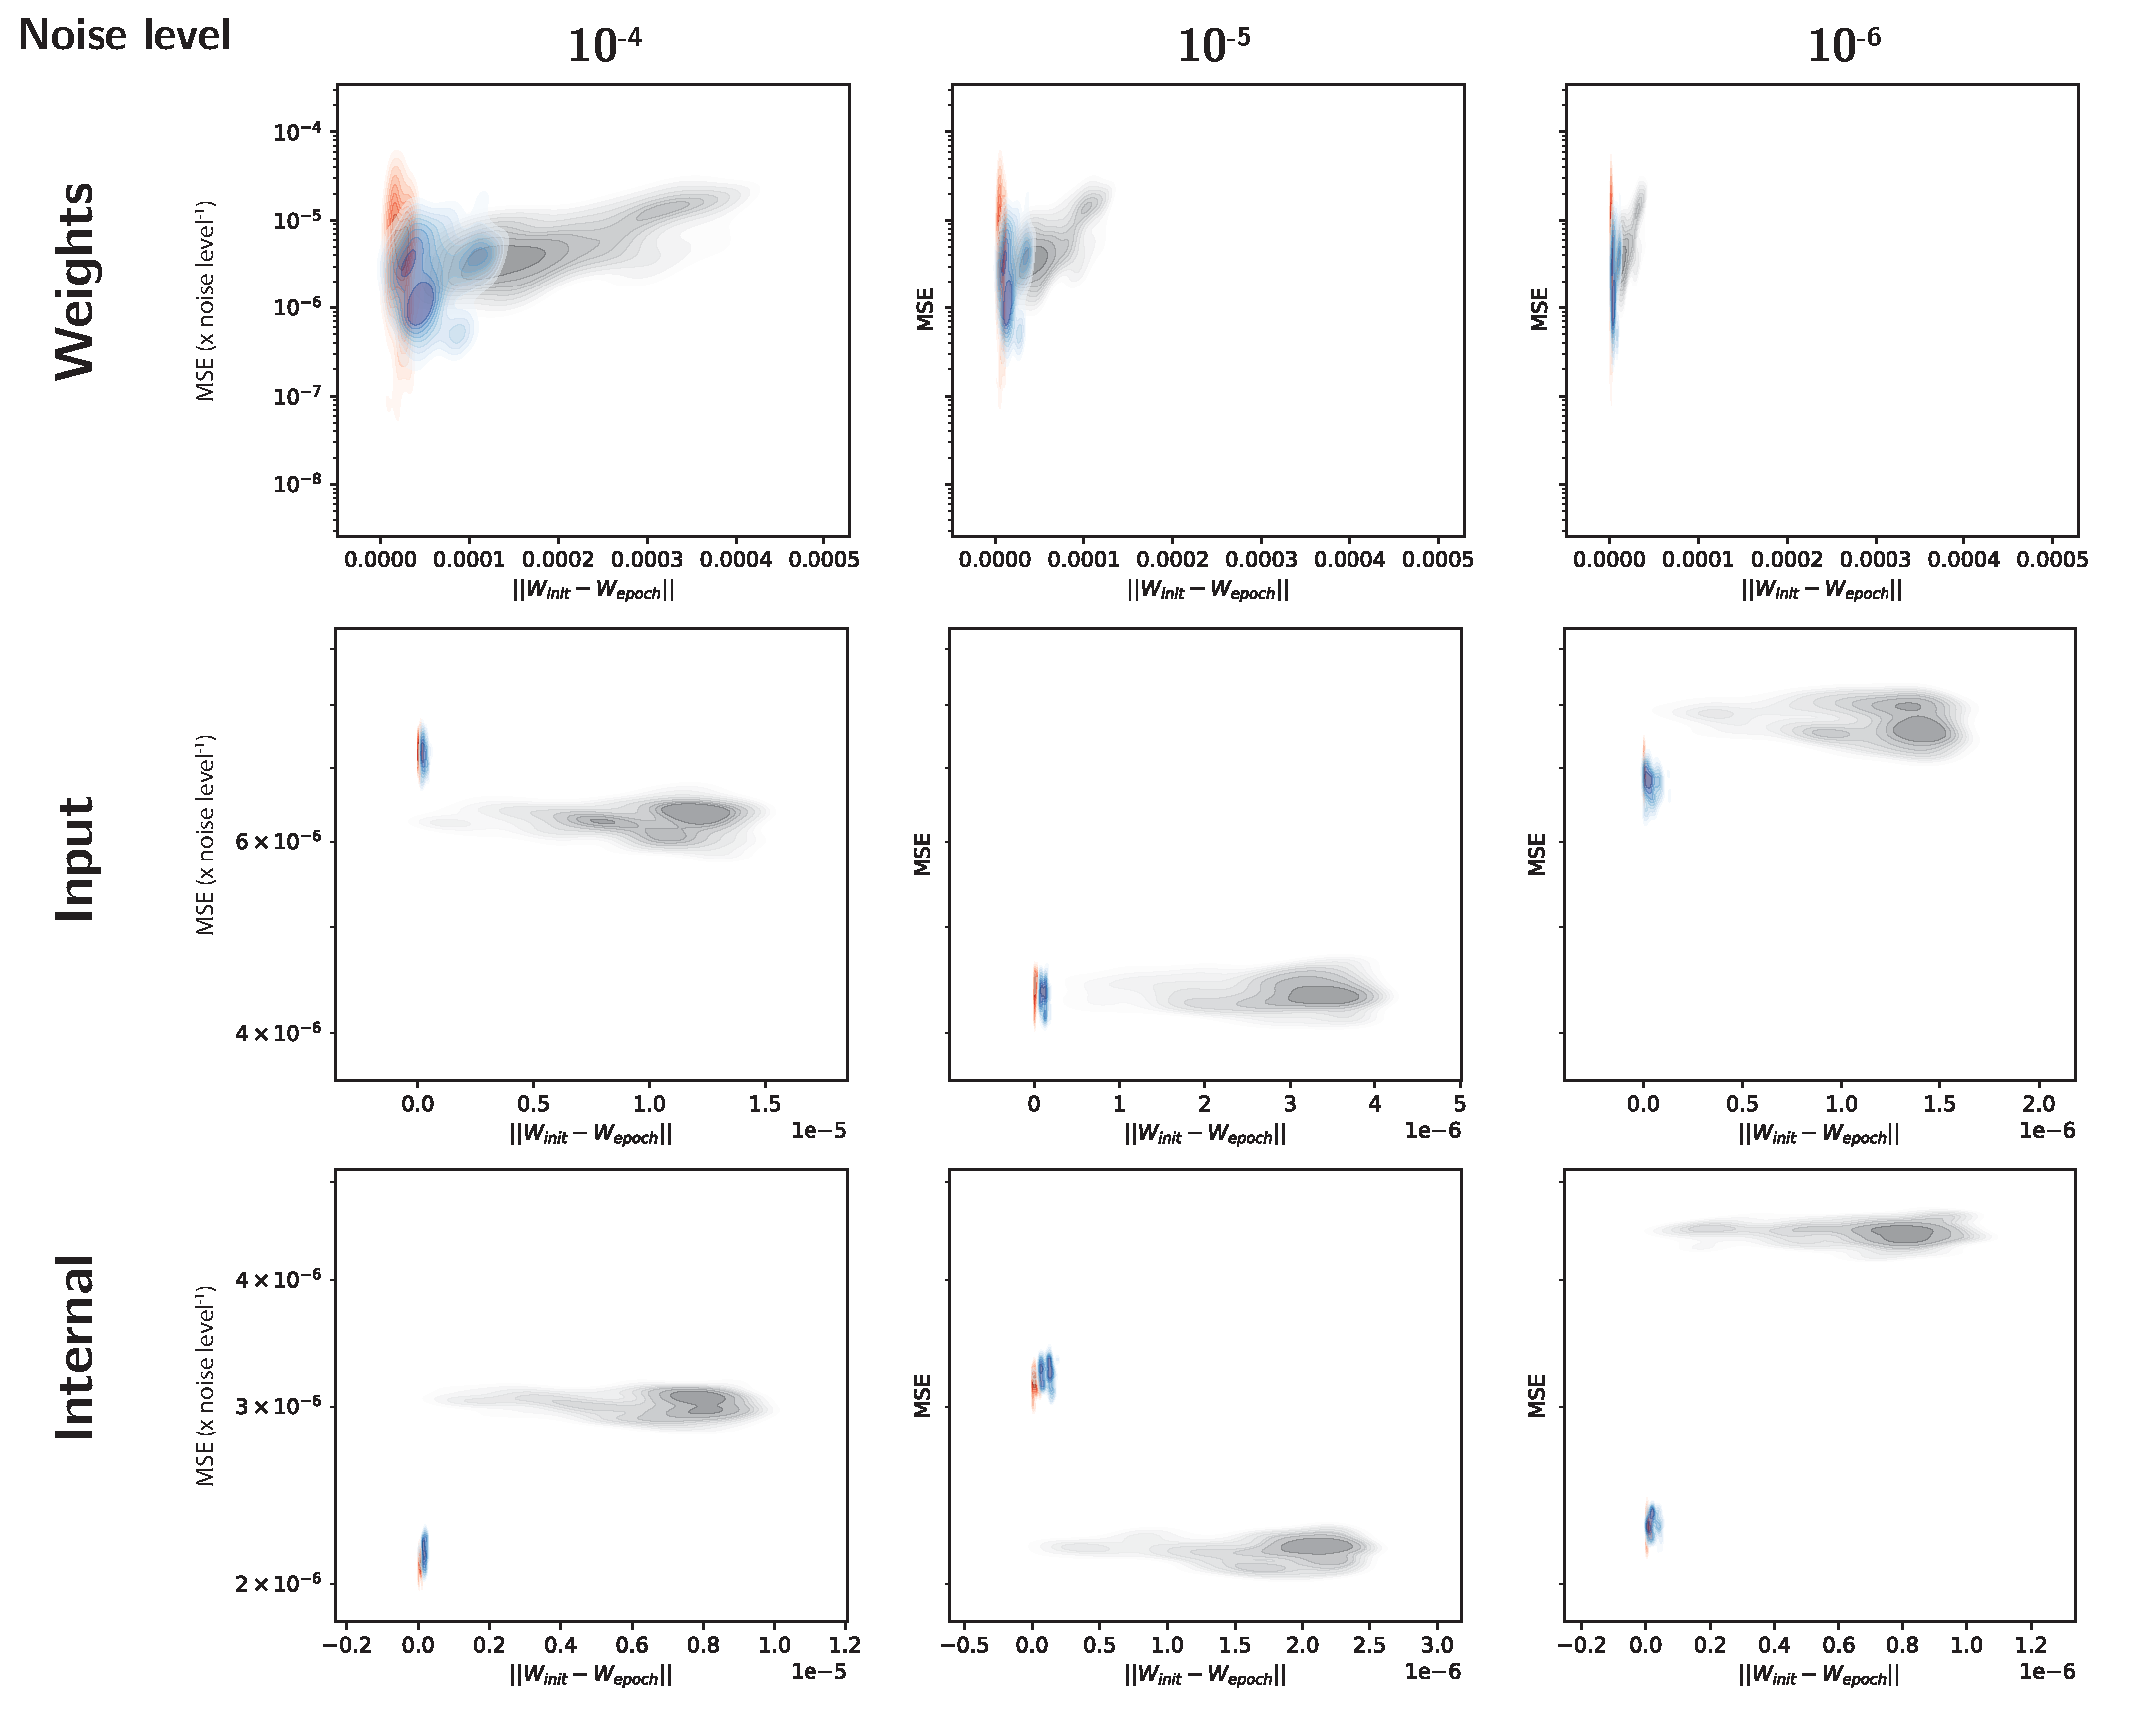
\includegraphics[width=\textwidth]{allnoise_contours}
%       \caption{Distribution of parameters for the three noise types for three noise levels. Because of relative scale of perturbation, iRNN is further away from the initial parameters with internal and input noise.
%        Depending on the level of the noise it performs better or worse than the LAs.}
%         \label{fig:interal_input_contours}
%\end{figure}
%
%
%\newpage
%\section{Changes to the neural integrators during learning}\label{sec:supp:learning}
%%Message: This is what happens to the different neural integrators during learning 
%During learning, the various neural integrators undergo distinct changes. These alterations manifest differently depending on the specific integrator involved. Here are some examples of progresses of chaning slow manifold dynamics.
%
%\begin{figure}[H]
%     \centering
%    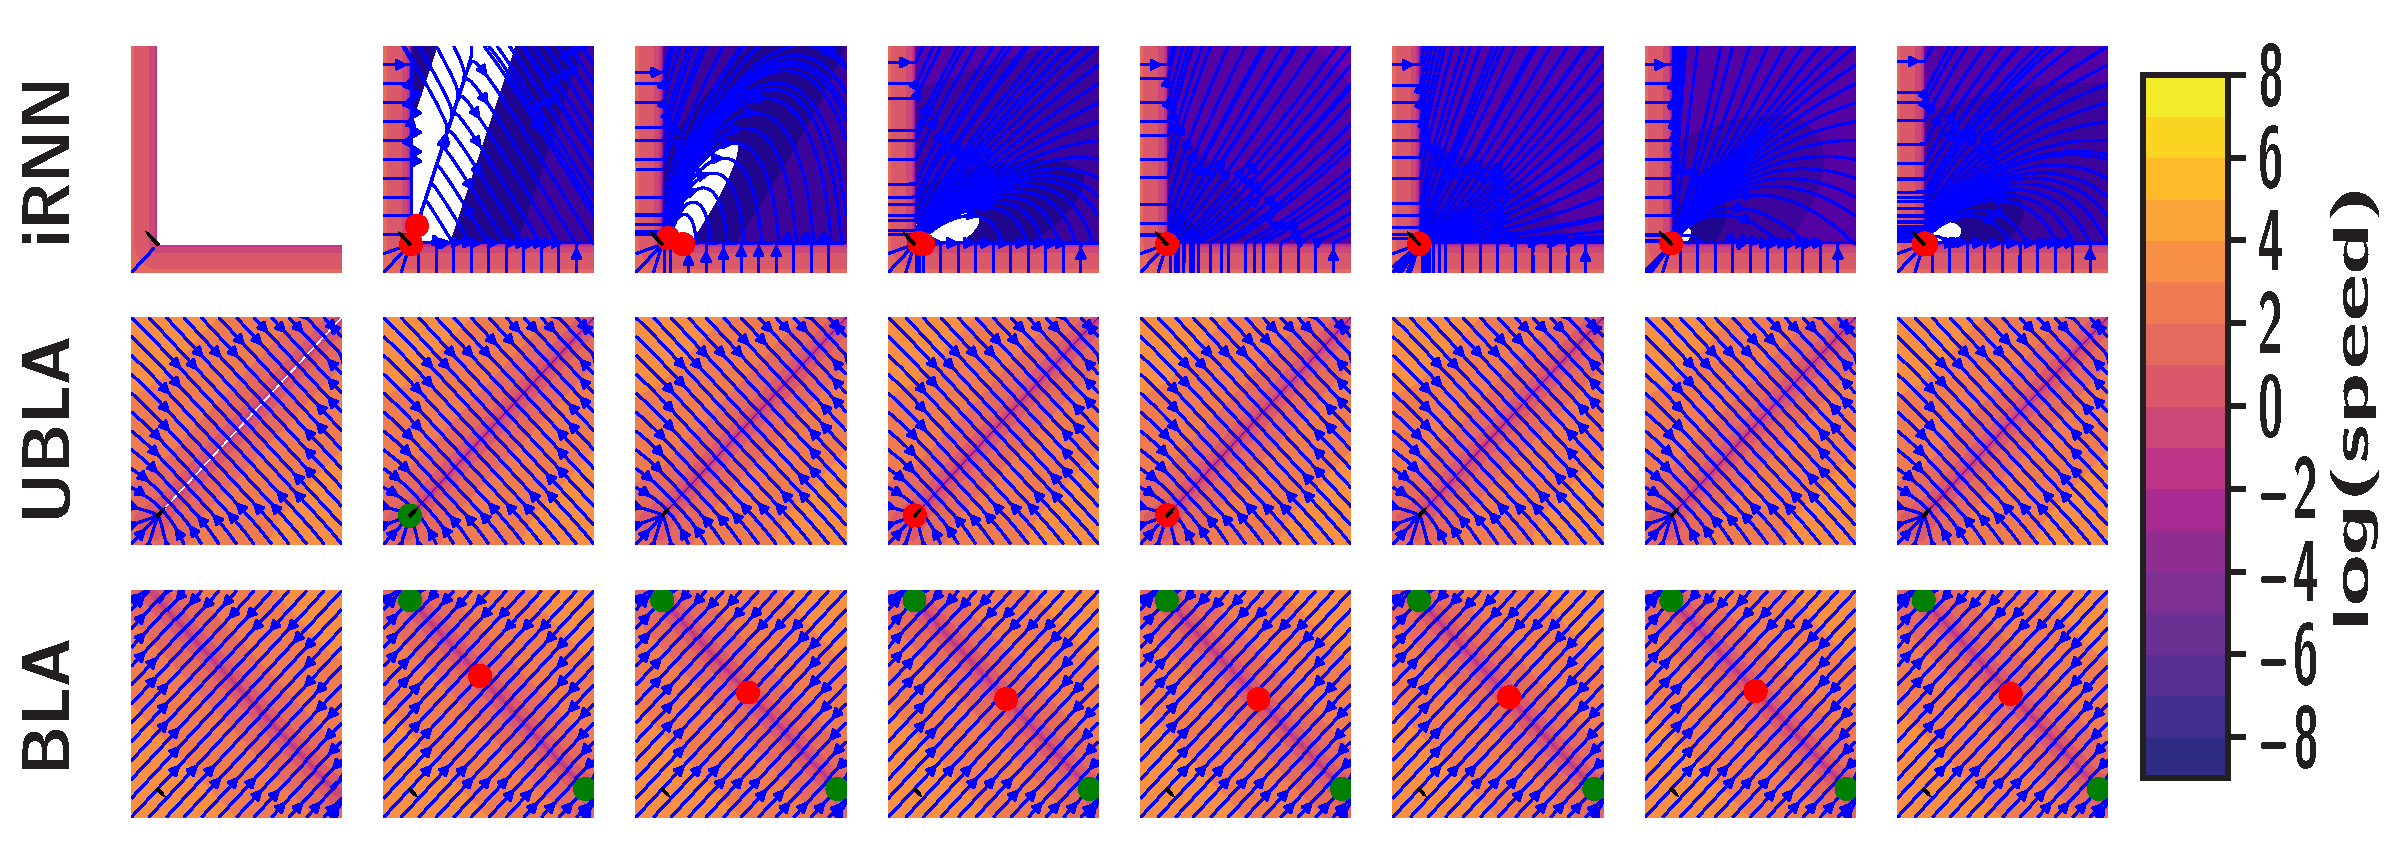
\includegraphics[width=\textwidth]{vfs_f100_gs1_optlrs}
%       \caption{The dynamics of the recurrent part of the integrators across learning with some example orbits (blue lines), stable (green) and unstable (red) fixed points. A gradient step is taken after every perturbation. Gradient steps 0, 1, 5, 10, 15, 20, 25 and 29 are shown. }
%         \label{fig:vfs1}
%\end{figure}
%
%\begin{figure}[H]
%     \centering
%    \includegraphics[width=\textwidth]{vfs_f100_gs5_optlrs}
%       \caption{The dynamics of the recurrent part of the integrators across learning with some example orbits (blue lines), stable (green) and unstable (red) fixed points. A gradient step is taken after every 5 perturbations. Gradient steps 0, 1, 5, 10, 15, 20, 25 and 29 are shown. }
%         \label{fig:vfs5}
%\end{figure}
%
%\begin{figure}[H]
%     \centering
%    \includegraphics[width=\textwidth]{vfs_f100_gs30_optlrs}
%       \caption{The dynamics of the recurrent part of the integrators across learning with some example orbits (blue lines), stable (green) and unstable (red) fixed points. 30 gradient steps are take after a single perturbation. Gradient steps 0, 1, 5, 10, 15, 20, 25 and 29 are shown. }
%         \label{fig:vfs30}
%\end{figure}
%
%
%\begin{figure}[H]
%     \centering
%    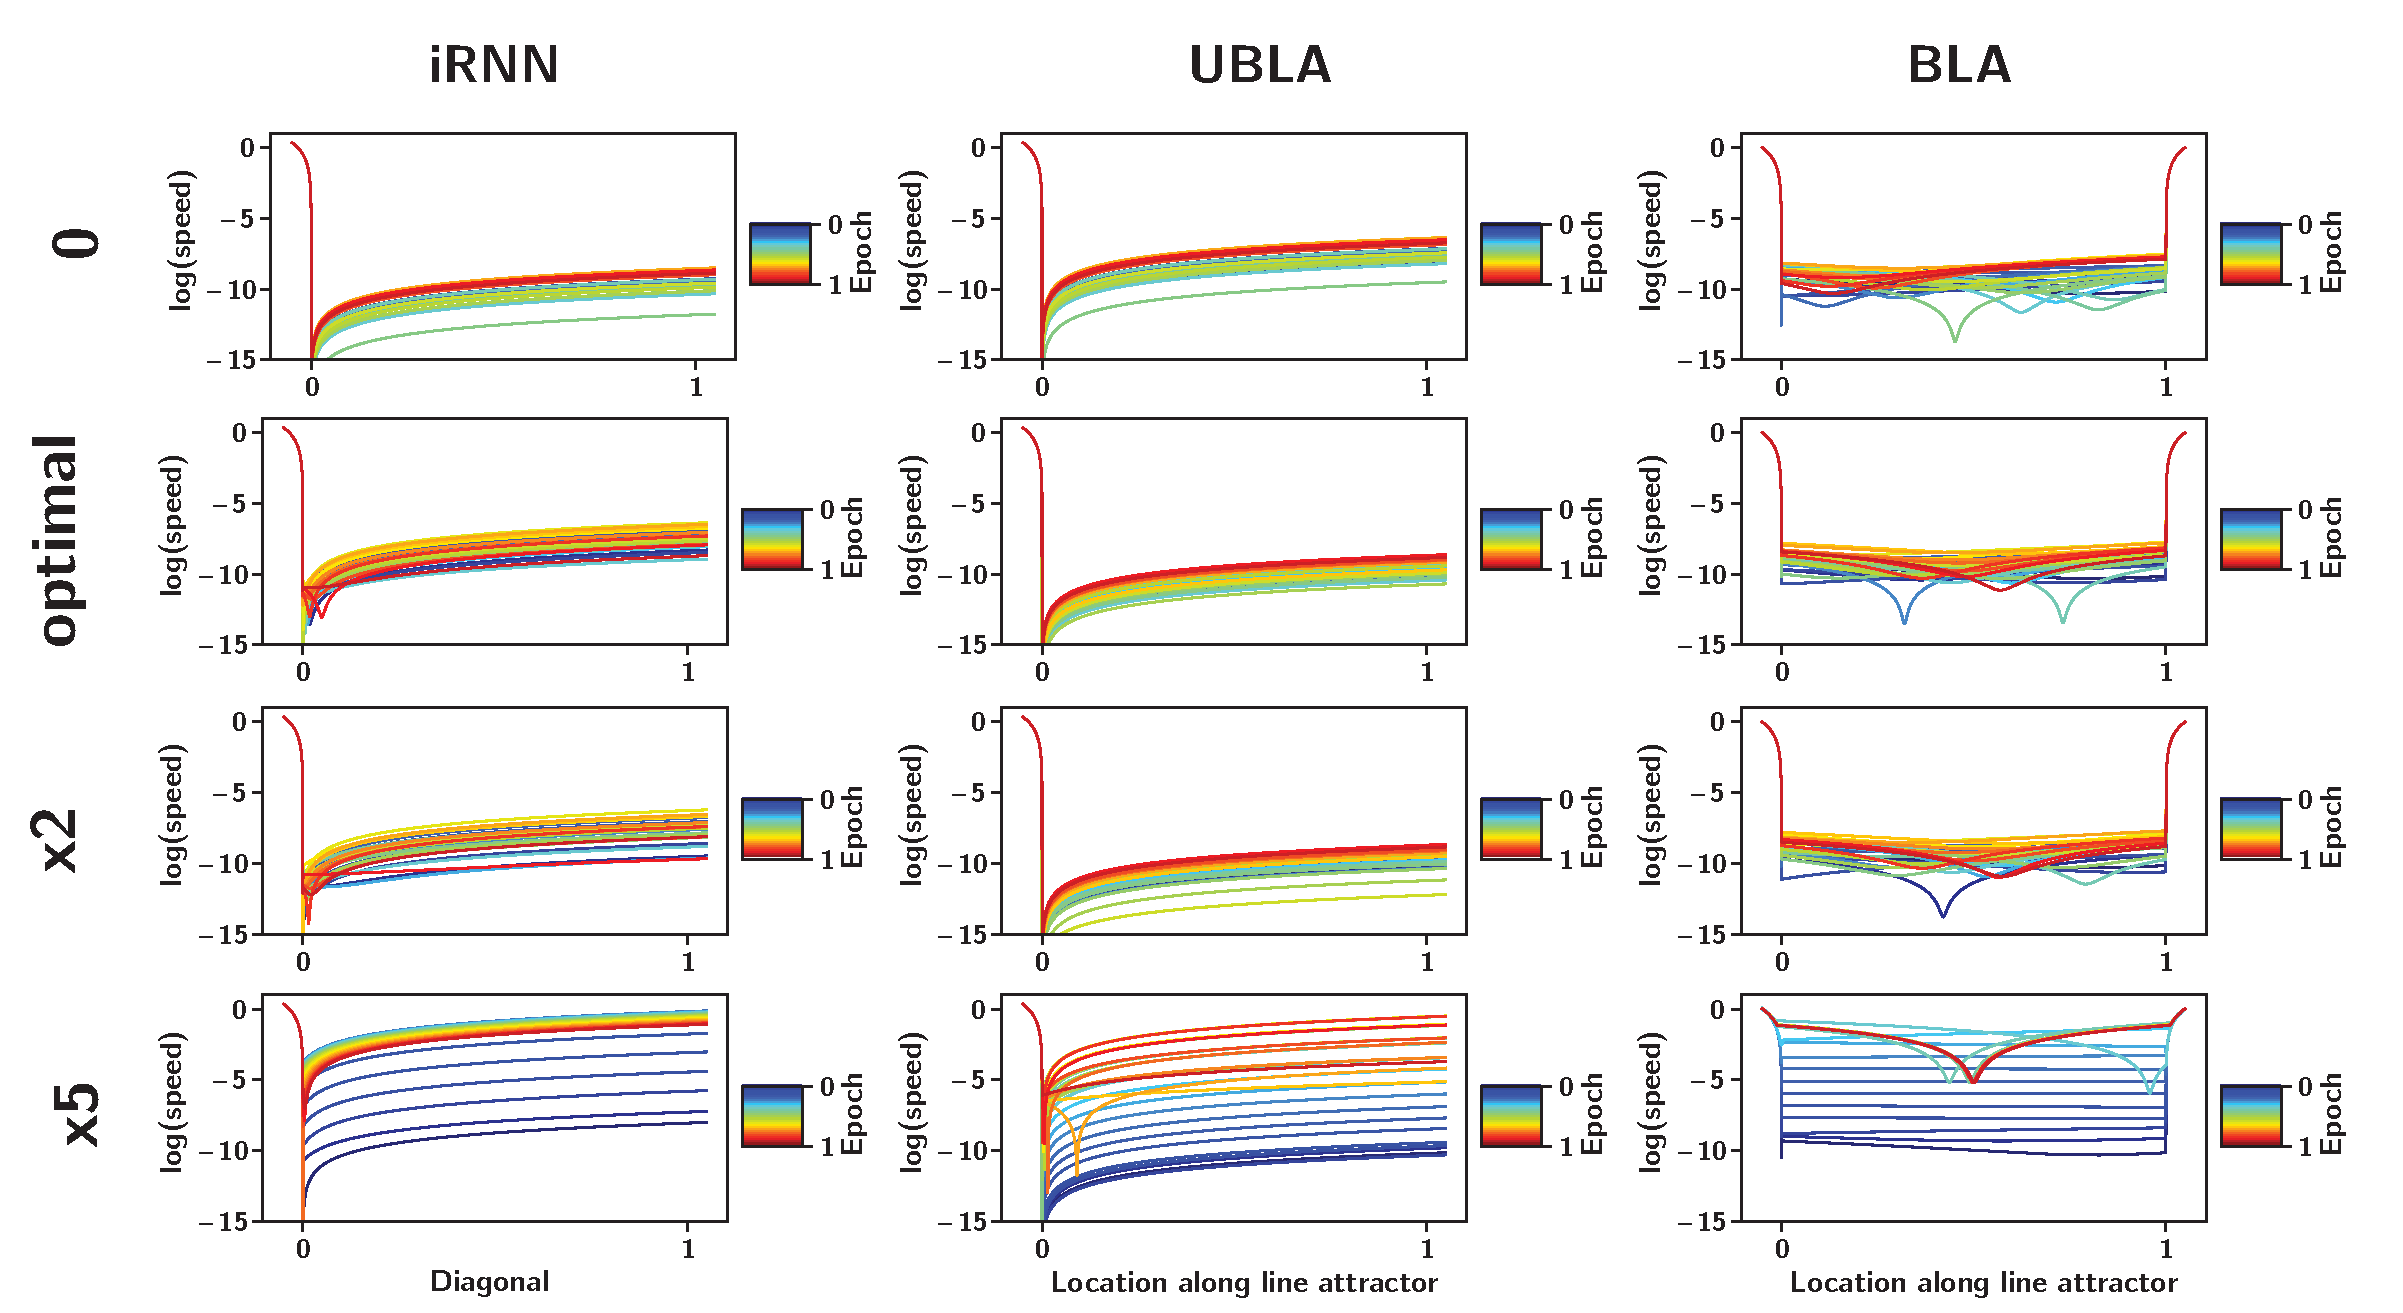
\includegraphics[width=\textwidth]{speeds}
%       \caption{Speed along the invariant manifold during learning. For the iRNN a slice (the diagonal) is shown.
%       %UBLA has a lower
%       }
%         \label{fig:speeds}
%\end{figure}

%%%%%%%%%%%%%%%%%%%%%%%%%%%%%%%%%%%%%%%%%%%%%%%%%%%%%%%%%%%%%%%%%%%%%%%%%%

%\section{Ring attractor}
%
%%Compact
%%No boundary: in- and outflowing
%%But not $C^1$!
%%
%%
%%discrete attractors as a trivial application?
%%Discrete attractors can be seen as an approximation to continuous attractor models in the context of head direction representation \citep{zhang1996}. The discrete nature of the representation makes it more robust to small fluctuations or disturbances in neural activity.
%%However, these system have fading memory: the system eventually forgets the past, since any difference between any two neural activations eventually tends zero as they both evolve to a global resting state.
%
%We will first of all look at a simple (non-biological) system that has a ring attractor to demonstrate the consequences of the Persistence Theorem.
%The system we will analyse is defined by the following ODE: $\dot r = r(1-r), \ \dot \theta = 0.$
%This system has as fixed points the ring with radius one centered around zero, i.e., $(0,0)\cup\{(1,\theta)\ |\ \theta\in[0,2\pi)\}$.
%
%
%\begin{figure}[H]
%     \centering
%%  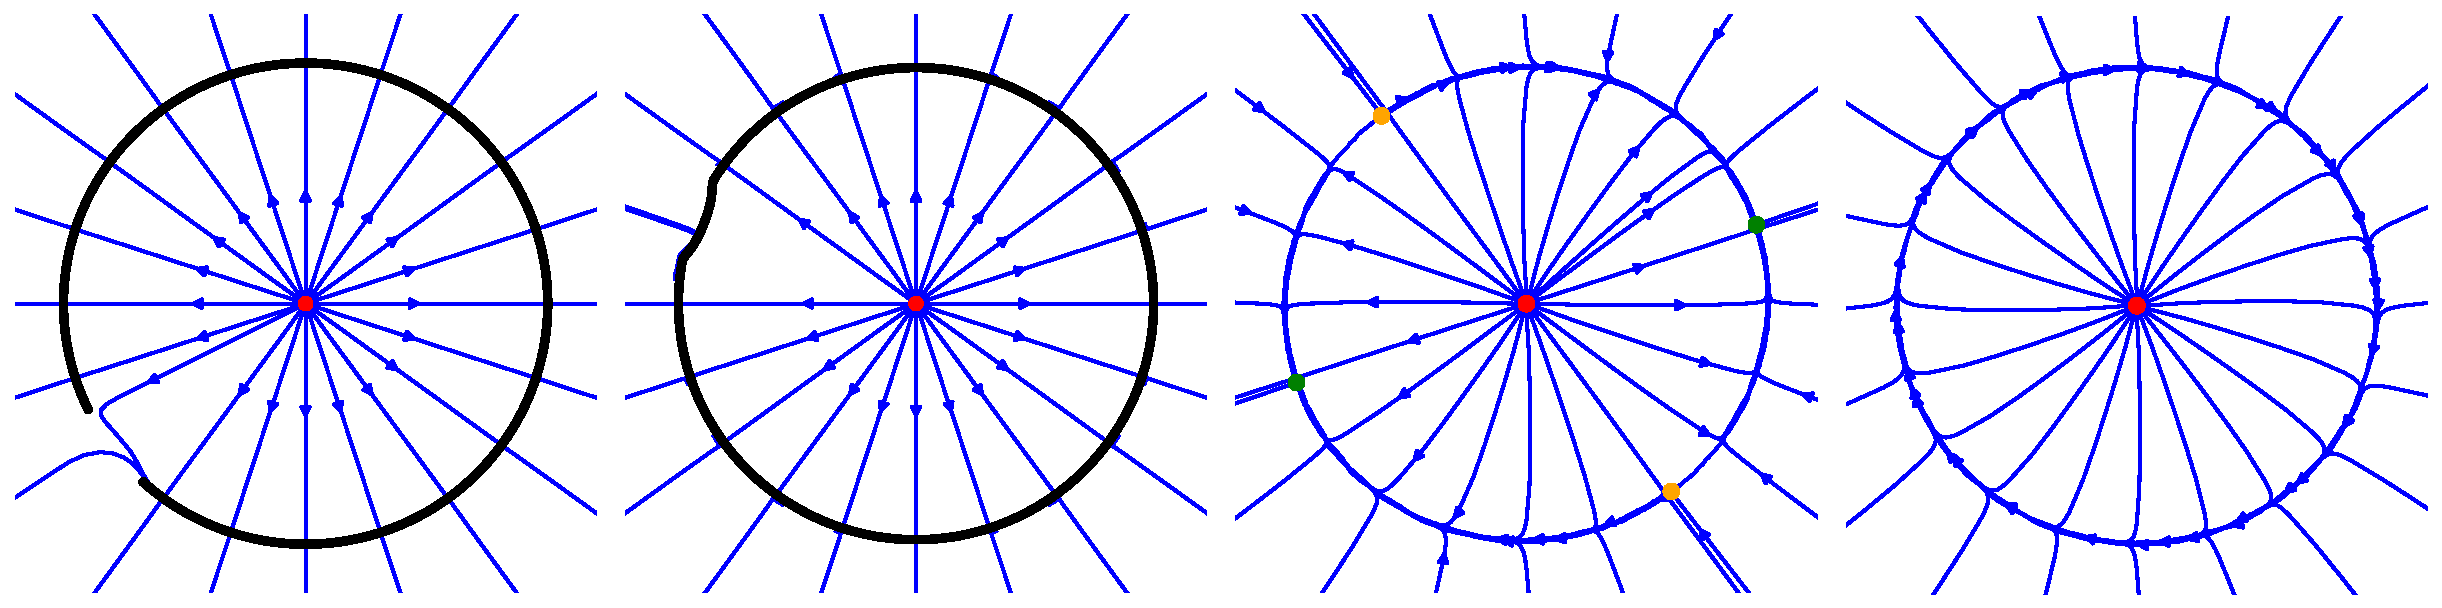
\includegraphics[width=.8\textwidth]{ring_perturbations_stream}
%    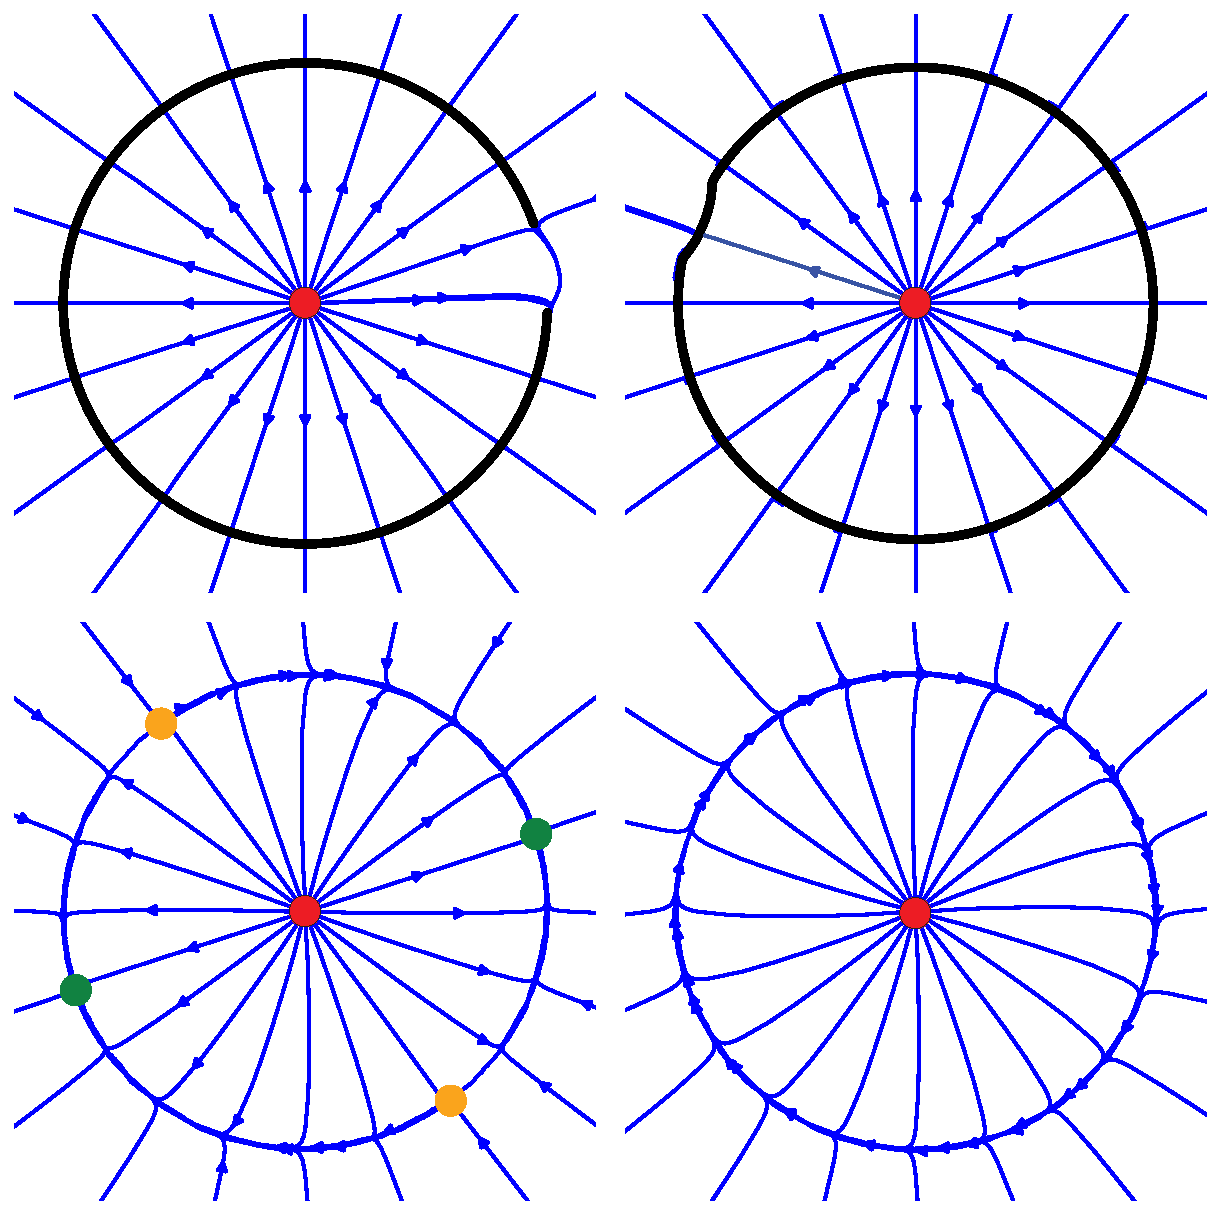
\includegraphics[width=.8\textwidth]{ring_perturbations_stream_2by2}
%       \caption{Perturbations to a simple implementation of a ring attractor all leave the invariant manifold intact. % (Left)  Examples of a local perturbation to the vector field through the addition of a bump to the vector field along the ring attractor.
%              (Leftmost) An example of a bump perturbation that results in the ring breaking up and becoming diffeomorphic to a line. %slow flow in hole?
%              (Left, middle) An example of a bump perturbation that maintains the ring structure, but deforms it locally.
%              %
%      % (Right) Examples of a global perturbation to the vector field through the addition of a small term to the connectivity matrix. 
%       (Right, middle) A global perturbation that results in a system with four fixed points along the persistent invariant manifold. %The two saddle nodes (yellow dots) are connected to the stable fixed points (green dots) through connecting orbits.
%       (Rightmost)   A global perturbation that results in a limit cycle.}
%         \label{fig:ring_activity_pert}
%\end{figure}

%All perturbations maintain the invariant manifold.






\newpage
\section{Ring perturbations}\label{sec:supp:ring_perturbations}

%Definition of a bump perturbation
We define a local perturbation (i.e., a change to the ODE with compact support) through the bump function $\Psi(x) = \exp\left(\frac{1}{\|x\|^2-1}\right)$ for $\|x\|<1$ and zero outside, by multiplying it with a uniform, unidirectional vector field. All such perturbations leave at least a part of the continuous attractor intact and preserve the invariant manifold, i.e. the parts where the fixed points disappear a slow flow appears.
%Definition of a global perturbation
The parametrized perturbations are characterized as the addition of random matrix to the connection matrix. 



\subsection{Simple ring attractor}
%Ring attractor
We further analyzed a simple (non-biological)  ring attractor, defined by the following ODE: $\dot r = r(1-r), \ \dot \theta = 0.$
This system has as fixed points the origin and the ring with radius one centered around zero, i.e., $(0,0)\cup\{(1,\theta)\ |\ \theta\in[0,2\pi)\}$.
We investigate bifurcations caused by parametric and bump perturbations of the ring invariant manifold (see Sec.~\ref{sec:supp:ring_perturbations}), which is bounded and boundaryless.
All perturbations maintain the topological structure of the invariant manifold . %(Fig.~\ref{fig:lara_bifurcations}B).
%include fig?

\subsection{Heading direction network}\label{sec:supp:headdirection}

\begin{equation}
\tau \dot h_j = -h_j + \frac{1}{N} \sum_k (W^{sym}_{jk} + v_{in} W^{asym}_{jk})\phi(h_k)+c_{ff},     j=1,\dots,N,
\end{equation}

In the absence of an input ($v_{in}=0$) fixed points of the system can be found analytically by considering all submatrices $W^{sym}_\sigma$ for all subsets $\{\sigma\subset [n]\}$ with$[n]=\{1,\dots, N\}$.
A fixed point $x^*$ needs to satisfy
\begin{equation}
x^*= -(W^{sym}_\sigma)^{-1}c_{ff}
\end{equation}
and 
\begin{equation}
x^*_i<0 \text{   for  	 } i\in\sigma.
\end{equation}

We bruteforce check all possible supports to find all fixed points.
We use the eigenvalues of the Jabobian to identify the stability of the found fixed points.


\subsubsection{Measure zero co-dimension 1 bifurcations}

\begin{figure}[tbhp]
     \centering
    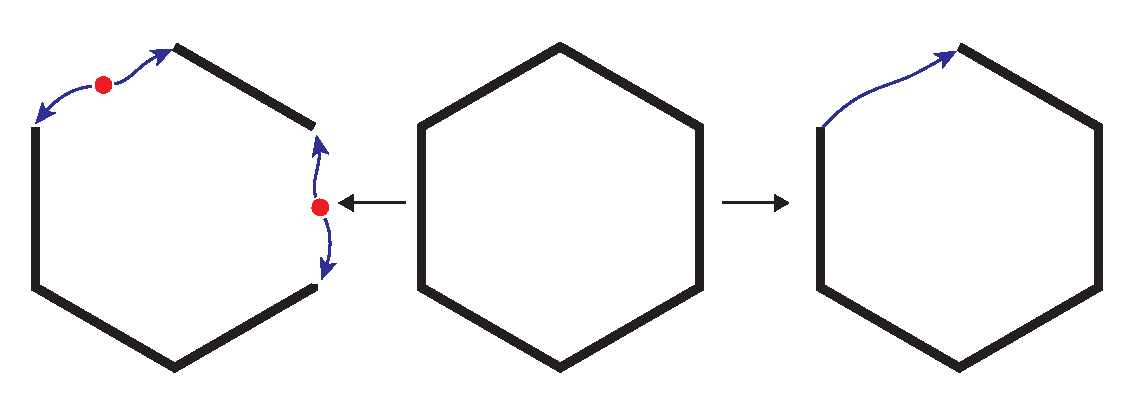
\includegraphics[width=\textwidth]{ring_n6_perturbations_schematic}
       \caption{Measure zero co-dimension 1 bifurcations of the ring attractor network \citep{Noorman2022}.}
         \label{fig:meaure_zero_perturbations}
\end{figure}


\subsubsection{Measure zero co-dimension $N$ bifurcation}
The limit cycle is the only bifurcation that we found that can be achieved on only a measure zero set of parameter values around the parameter for the continuous attractor.






\subsubsection{Independence of norm of perturbation on bifurcation}

\begin{figure}[tbhp]
     \centering
    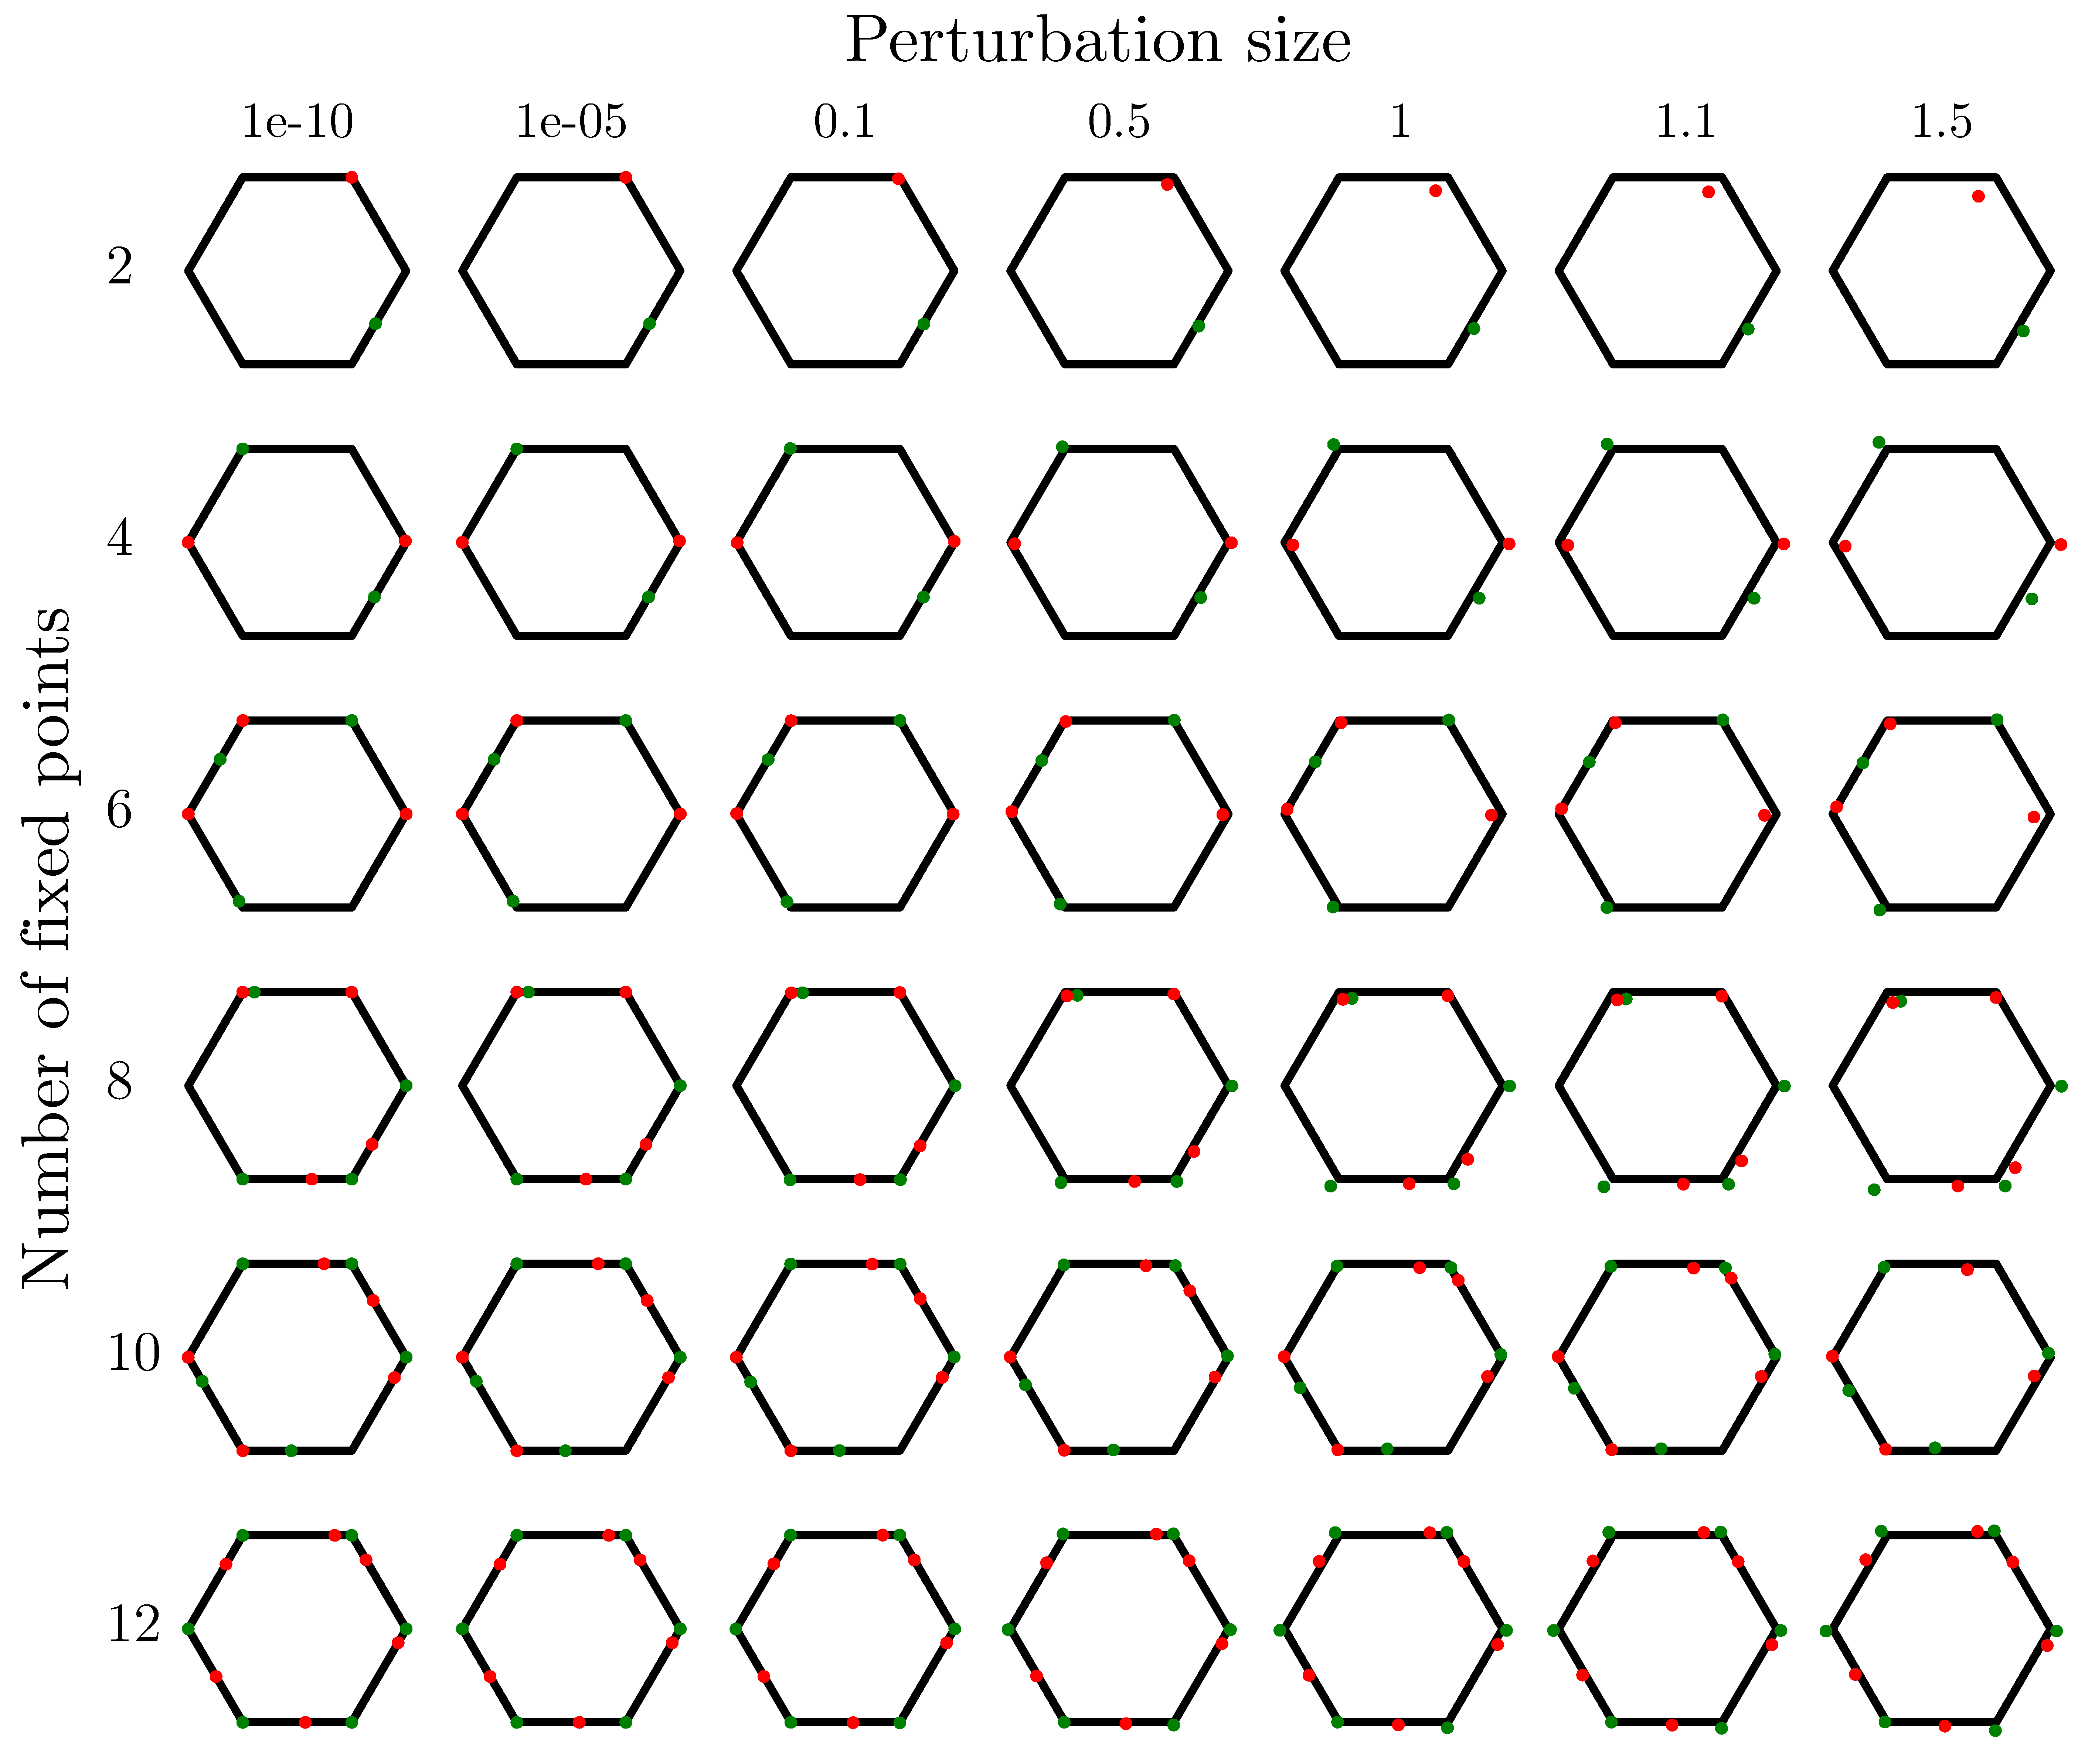
\includegraphics[width=\textwidth]{noorman_ring_N6_pert_allfxdpnts_allnorms}
       \caption{Rows show the bifurcations resulting from perturbations from the matrices with the same direction in Fig.~\ref{fig:bio_rings}A but with different norms (columns). }
         \label{fig:noorman_ring_allfxdpnts_allnorm}
\end{figure}



\newpage
\subsection{Ring attractor approximation with tanh neurons}\label{sec:supp:goodridge}


We investigated the bifurcations around the approximate ring attractor constructed with a symmetric weight matrix for a tanh network  \citep{compte2000synaptic, seeholzer2017efficient}.
The functional form of $W$ is the sum of a constant term plus a Gaussian centered at $\theta_i - \theta_j =0$:
\begin{equation}
W(\theta_i - \theta_j) = J^- + (J^+ - J^-) \exp\left[ -\frac{(\theta_i - \theta_j)^2}{2\sigma^2} \right],
\end{equation}
with the dimensionless parameter $J^-$ representing the strength of the weak crossdirectional connections, $J^+$ the strength of the stronger isodirectional connections,
 and $\sigma$ the width of the connectivity footprint.
 
 
 Such ring attractor approximations are similar to the ones in \citep{goodridge2000, samsonovich1997path, redish1996coupled}. %Equation 9,12
 



\subsubsection{Loss of function: Sensitivity of continuous attractors to perturbations}\label{sec:supp:boa}

We will show that there are differences at how well approximations perform at different timescales.

\begin{figure}[tbhp]
  \centering
  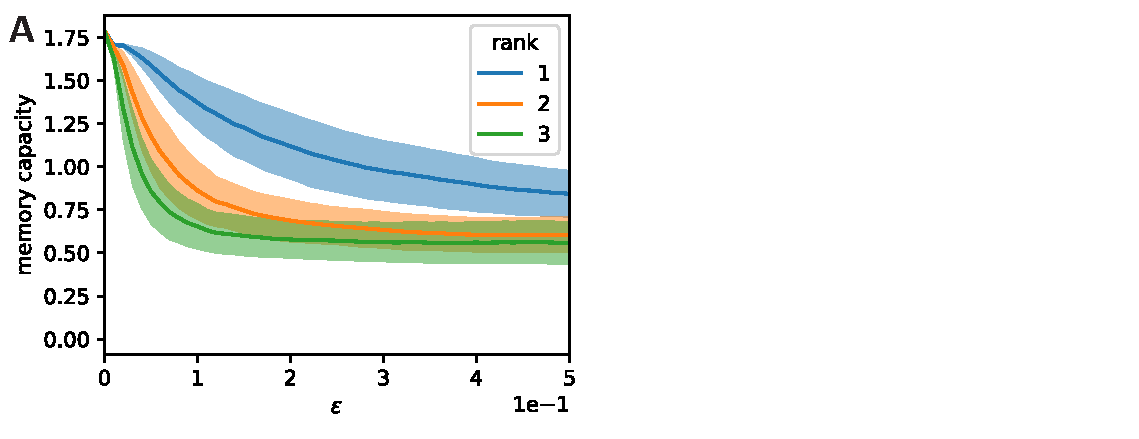
\includegraphics[width=\textwidth]{performance}
  \caption{Degradation of performance across perturbation sizes.
  (A) System behavior at the asymptotic time scales measured through memory capacity. }
  \label{fig:performance}
\end{figure}

%Networks
%  \citep{seeholzer2017efficient} %tanh
%  \citep{goodridge2000}		%sigmoid

We measure how performance of different models for the representation of an angular variable drop as a function of perturbation size Fig.~\ref{fig:performance} through the memory capacity metric.
For each perturbation size, we sample a low rank (rank 1,2 or 3) random matrix with norm equal to that perturbation size.
We determine the location of the fixed points through the local flow direction criterion as described in Sec.~\ref{sec:fastslowmethod}
and determine the basin of attraction
\begin{equation}
\basin(x^*) \coloneqq \{x\in \manifold \ | \lim_{t\rightarrow\infty}\varphi(t,x)=\{x^*\}\}.
\end{equation}
through assesing the local flow direction for 1024 sample points in the found invariant manifold.
This invariant manifold was found to be consistently close the the original invariant ring attractor.
The initial ring had $2N$ fixed points ($N$ stable, $N$ saddle) on this invariant ring manifold.
The memory capacity of this initial configuration is $N\log(N)$ for the $2N$ uniformly spaced fixed points.


%\subsection{Couey}\label{sec:supp:couey}
%\citep{couey2013}
%
%\subsection{NEF}
%\citep{barak2021mapping}


\subsection{Low-rank}\label{sec:supp:lowrank}


The networks consisted of $N$ firing rate units with a sigmoid inputoutput transfer function \citep{mastrogiuseppe2018}
\begin{equation}
\xi_i(t) = - \xi_i(t) + \sum_{j=1}^{N} J_{ij}\phi(x_j(t)) + I_i
\label{eq:1}
\end{equation}
where $x_i(t)$ is the total input current to unit $i$,
$ J_{ij} = g\chi_{ij} + P_{ij}$ is the connectivity matrix, 
$\phi(x) = \operatorname{tanh}(x)$ is the current-to-rate transfer function, and $I_i$ is the external, feedforward input to unit $i$.

This far we focused on unit-rank connectivity structure, but our framework can be directly extended to higher-rank structure. A more general structured component of rank $r\ll N$ can be written as a superposition of $r$ independent unit-rank terms 
\begin{equation}
P_{ij} = \frac{m^{(1)}_i n^{(1)}_j}{N} + \dots + \frac{m^{(r)}_i n^{(r)}_j}{N},
\end{equation} and is in principle characterized by $2r$ vectors $m^{(k)}$ and $n^{(k)}$.
$g\chi$ is considered unknown except for its statistics (mean 0, variance $g^2/N$).

$N=10,100,1000$
$\Sigma=2$
$\rho=1.9$
$g=0, 0.1$


\begin{figure}[h]
\centering
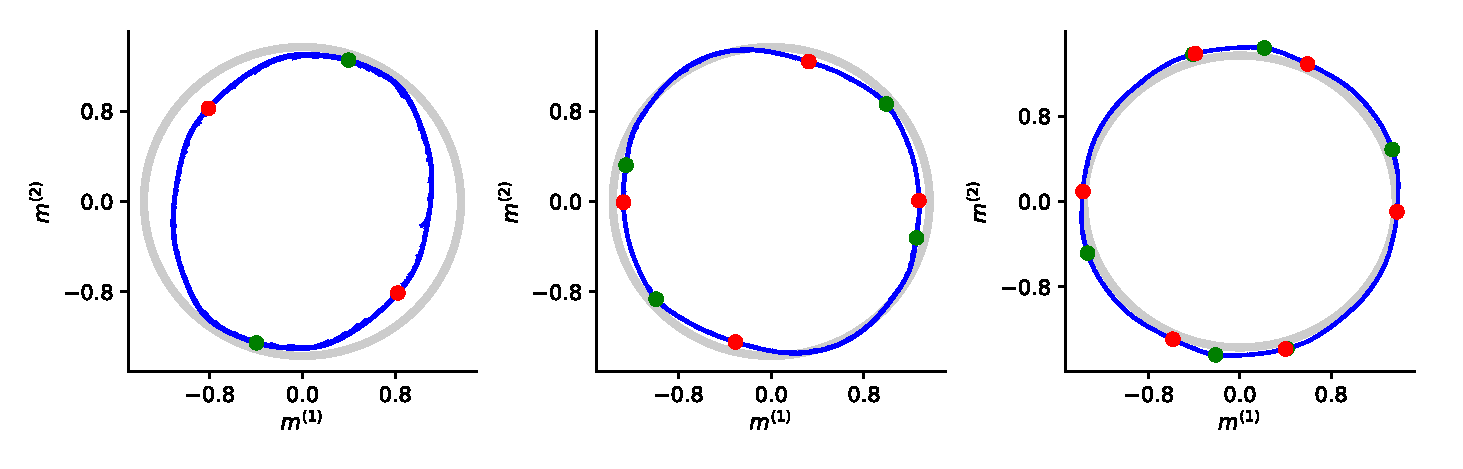
\includegraphics[width=0.8\textwidth]{N100_si2_rho1.9_g0_fp4.8.12}
\caption{Some examples of networks dynamics.}
\label{fig:low_rank_examples}
\end{figure}


\subsection{EMPJ}\label{sec:supp:empj}
We fit 3 networks with the Embedding Manifolds with Population-level Jacobians (EMPJ) method \citep{pollock2020}.
We take a ring and embed it with a random linear mapping to a 10 dimensional state space.
On this embedded ring, we constraint the network to have evenly spaced fixed points with one marginal Jacobian eigenvalue and all others eigenvalues -20.



%\newpage
%\subsection{Biswas}\label{sec:supp:biswas}




%\newpage
%\section{Training RNNs on an integration task from scratch}
%
%We trained vanilla RNNs with a ReLU nonlinearity for the recurrent layer and a linear output layer on the angular velocity integration task Fig.~\ref{fig:angular_task}. The network size varies between 50 and 200 units, initialized using a normal distribution for the parameters. Adam optimization with $\beta_1=0.9$ and $\beta_2=0.99$ was employed with a batch size of 512 and training was run until no decrease in the loss occurred for 100 epochs. The task has 256 time steps for the training samples, and training was based on the mean squared error loss.
%
%\begin{figure}[tbhp]
%     \centering
%    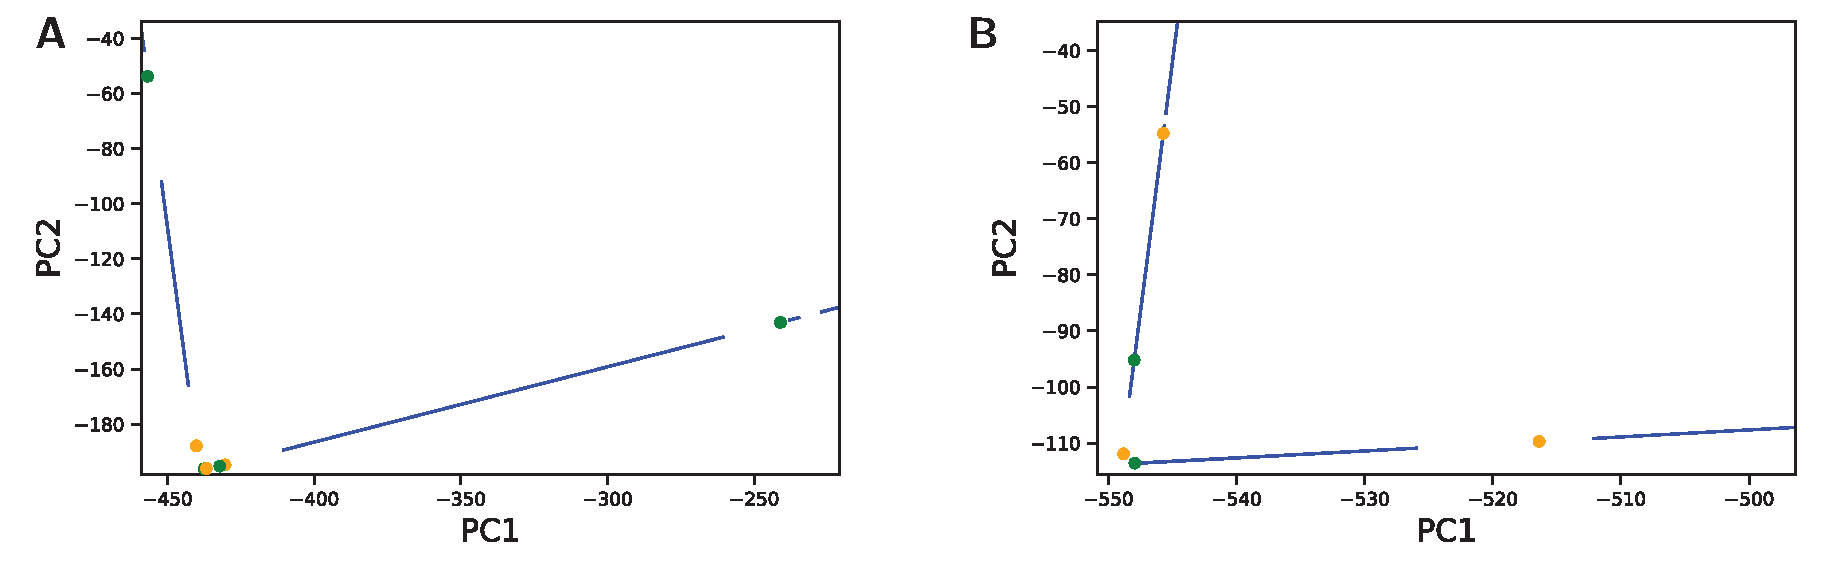
\includegraphics[width=\textwidth]{line_attractor_like_solutions}
%       \caption{The two types of found solutions. A) A line attractor with hyperbolically stable fixed points at the end of the line. B) Saddle nodes at the ends of the line.
%}
%         \label{fig:line_att_sols}
%\end{figure}
%
%From an arbitrary initialization, we find that a line attractor-like structure often (8 out of 10 runs) emerged with hyperbolically stable fixed points (Fig.\ref{fig:line_att_sols}A) when trained on a longer version of the task. For shorter trial lengths, saddle nodes are more likely to emerge (6 out of 10 runs) at the ends of the line (Fig.~\ref{fig:line_att_sols}B), meaning that the resulting structure is not an attractor. 
%



\newpage
\newpage
\section{Tasks}\label{sec:supp:tasks}
%Inputs and outputs for an example trial on each task are shown in Supp.Fig.~\ref{fig:supp:tasks}.


\paragraph{Memory guided saccade task}

The total time length of the task was 512 steps.
The time delay to the output cue was sampled from 
\begin{align}
T_{delay} \sim \mathcal{U}(50, 400).
\end{align}
We applied a mask $m_{i,t}=0$ for 5 time steps ($T_{delay}+i$ for $i=0,\dots 4$) after the go cue.



\paragraph{Angular velocity integration task}
The input is an angular velocity and the target output is the sine and cosine of the integrated angular velocity.
Velocity at every timestep  is sampled from as a Gaussian Process (GP) for smooth movement trajectories, consistent with the observed animal behavior in flies and rodents.
%These parameters are set to roughly match the angular velocity distribution of the rat and fly (Stackman & Taube, 1998; Sharp et al., 2001; Bender & Dickinson, 2006; Raudies & Hasselmo, 2012).
\begin{equation}
k(x,y)=\exp\left(-\frac{\|x-y\|}{2\ell^2}\right),
\end{equation}
with length scale $\ell$.
 The length scale of the kernel was fixed at 1.
 
 \begin{figure}[tbhp]
     \centering
    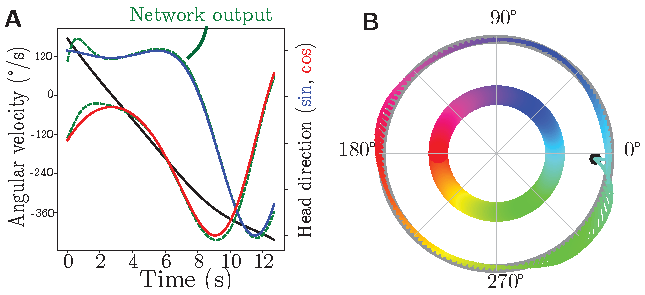
\includegraphics[width=0.75\textwidth]{task_fig}
       \caption{Description of the tasks. A) The angular velocity integration task. B) The output of the angular velocity integration in the output space, color coded according to the integrated angle. An example of an input is shown with constant velocity and it is provided until one turn is completed.}
         \label{fig:angular_task}
\end{figure}

 
 
 
 
 \section{Training methods}
 
 We trained vanilla RNNs with PyTorch \citep{paszke2017automatic} with a tanh nonlinearity for the recurrent layer and a linear output layer on the angular velocity integration task Fig.~\ref{fig:angular_task}.
 The network size is 20 units, initialized using a normal distribution for the parameters.
  Adam optimization with $\beta_1=0.9$ and $\beta_2=0.99$ was employed with a batch size of 512 and training was run until no decrease in the loss occurred for 1000 epochs.
   The task has 100 time steps for the training samples, and the mean squared error loss was used.
The batches were generated on-line, similar to how animals are trained with a new trial instead of iterating through a dataset of trials.

The best learning rate was chosen from 5 initial runs for all networks.
Training a single network took around 10 minutes on a CPU and occupied 10 percent of an 8GB RAM.

 \section{RNN analysis methods}
 
 %fast-slow
 % inv man
 
 \subsection{Fast-slow decomposition}
 We simulated 1024 trajectories without noise with inputs from the task and let the networks evolve for 16 times the task definition lengths.
 We took the cutoff to identify the slow manifold to be $10^{-3}$ of the highest speed along each trajectory.
 We believe that this gaurantees the identification of the slow manifold in a system that has a fast-slow decomposition.	
 We sampled 1024 points from these points to fit a periodic, cubic spline (black line in Fig.\ref{fig:fastslow_decomposition}).
 
 \subsection{Vector field on invariant manifold}\label{sec:supp:vf}
 
 We assess the vector field for the ODE (Eq.~ \ref{eq:RNN:continuous} without noise and input) on the found invariant manifold $\manifold$ by calculating it in the state space
 and then projecting it onto the output space:
 \begin{equation}
\dot \alpha =  \wout f(\hat \alpha) %=: g(\alpha)
\end{equation}
for sampled points $\hat \alpha\in \manifold$.
These points $\hat \alpha\in \manifold$ on the manifold are associated with the points on the ring through the mapping $\alpha = \wout\hat\alpha$.
 
  
 \begin{figure}[tbhp]
     \centering
    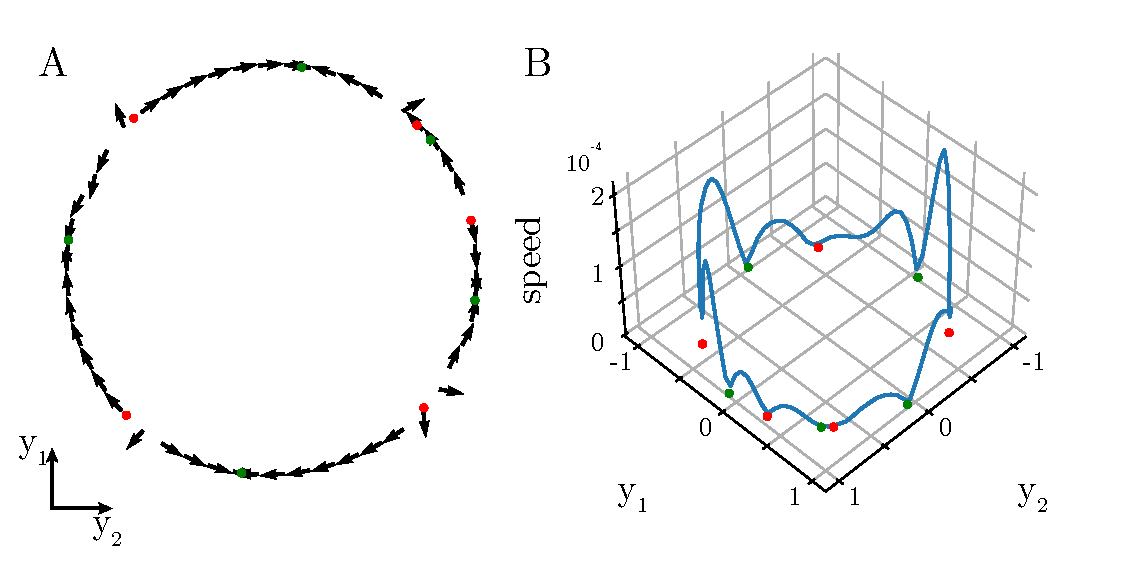
\includegraphics[width=\textwidth]{vf_on_ring}
       \caption{The projected vector field on the found invariant manifold for the system Fig~\ref{fig:fastslow_decomposition}C.
       (A) The found vector field aligns well with the ring in the projected output space.
       (B) The norm of the vector field is low around found fixed points as expected, but is higher for points that are just slow points.
       }
         \label{fig:vf_on_ring}
\end{figure}
 
This vector field in the output space captures in what direction and how quickly angular memory will decay. 
 The vector field  suggests that the system indeed has an invariant manifold (Fig. \ref{fig:vf_on_ring}).
 Furthermore, the vector field and fixed points are consistent with each other, as the vector field flips direction around found fixed points.

 
 There are some inconsistencies around saddle nodes, where the vectori field seems to point off of the manifold.	
 This is probably just inaccuracies  coming from numerically calculating the vector field and the exact location of the invariant manifold.
%
For the bound discussed in Sec.~\ref{sec:revival}, we calculate the uniform norm of the found vector field $\|f\|_\infty = \sup f(\alpha)$ (see also Sec. \ref{sec:app:bouding}).

%
%
%\begin{figure}[tbhp]
%     \centering
%    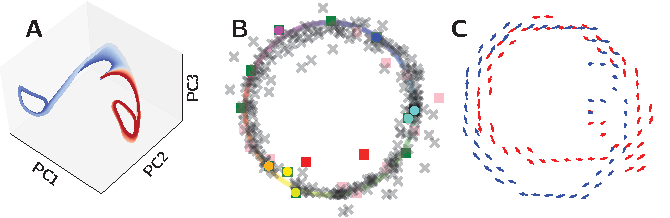
\includegraphics[width=\textwidth]{analysis_small}
%       \caption{Analysis steps for the distillation of the implemented computation in a trained RNN. A) Input driven hidden trajectories for constant inputs of different magnitudes in the left (blue) and right (red) direction. B) Projection onto the output space of the attractors found by simulation until convergence to periodic solutions (color indicates the angular direction it maps to) with slow points found by minimizing the speed of the hidden (square) or output (cross) dynamics. Stability is indicated by green for stable, pink and red for saddles with 1 and 2 unstable dimensions, respectively. C) Effective input drive shown as average vector fields for the hidden dynamics projected onto the output space. Averages taken for a single constant input in left (blue) and right (red) directions.}
%         \label{fig:asymptotic_analysis}
%\end{figure}
%
%\begin{figure}[tbhp]
%     \centering
%    \includegraphics[width=\textwidth]{example_solutions}
%       \caption{A) A solution with a single limit cycle (light blue) that gets mapped onto a small subset of the output space. B) A solution with multiple limit cycles spread around the ring attractor. C) A solution with only fixed points spread around a ring like attractor with slow dynamics.}
%         \label{fig:angular_solutions}
%\end{figure}
%
%
%For the angular velocity integration task, typical solutions have two limit cycles corresponding to the two directions of constant inputs. The autonomous dynamics can be characterized by an (approximate) line attractor with two (approximate) ring attractors at the ends. 
%The found solutions Fig.\ref{fig:angular_solutions}A-C all show bounded ring-like attractors. These solutions are all composed of two rings (Fig.\ref{fig:asymptotic_analysis}A) connected by an (approximate) line attractor.
%
%The vector field (Fig. \ref{fig:asymptotic_analysis}C) suggests that the system exhibits input driven dynamics  corresponding to a limit cycle, which would mean that the invariant manifold of the input-driven dynamics is compact.
%%\include{iclr2024_supplementary.tex}




\newpage

\section{Bounding the loss}\label{sec:app:bouding}
We formulate here a theory of continuous attractor approximations in terms of memory loss over time.

Let $\mathcal{U}\subset \mathbb{R}^D$ be a subamifold and  with metric $d(x,y): \mathcal{U} \times \mathcal{U} \rightarrow \mathbb{R}$.
%Then we have a dynamical system $\bm{x} \in \mathbb{R}^N$ with autonomous dynamics $\dot{ \bm{x}} = F_{\boldsymbol{\theta}} (\bm{x})$. 
Suppose that there is an encoder mapping $f: \mathcal{U} \rightarrow \mathbb{R}^N$ such that the inverse of this encoder mapping is a function (although not necessarily injective): $f^{-1}: Im(f) \rightarrow \mathcal{U}$. 
Then, let us define a memory loss in a time $T$ as:
\begin{equation}
    \mathcal{L}(T) = \frac{1}{|\mathcal{U}|} \int_\mathcal{U}  \frac{1}{|f(\bm{\alpha})|} \int_{f(\bm{\alpha})} \frac{1}{T} \int_0^T d(f^{-1}(\phi_{\bm{\theta}}(f(\bm{\alpha}),t),\bm{\alpha}) dt df(\bm{\alpha}) d\bm{\alpha}
\end{equation}

If $D = 1$, then without loss of generality we can take $\mathcal{U} = [a,b]$ (or open/closed combinations and/or $a = -\infty$ and/or $b = +\infty$):

\begin{equation}
    \mathcal{L}(T) = \left(\lim_{a(,b) \rightarrow -\infty(,+\infty)}\right) \frac{1}{b - a} \int_a^b  \frac{1}{|f(\alpha)|} \int_{f(\alpha)} \frac{1}{T} \int_0^T d(f^{-1}(\phi_{\bm{\theta}}(f(\alpha),t)),\alpha) dt df(\alpha) d\alpha
\end{equation}

\subsection{Ring attractor}

In the case of the ring attractor the memory we would like to encode is $\alpha \in \mathcal{U} = [0,2 \pi)$ and the error is defined as $d(x,y) = o_\pi(|x-y|)$ where:

\begin{equation}
    o_\pi(x) = \begin{cases}
    x & \text{if } x < \pi \\
    2 \pi - x & \text{if } x \geq \pi
    \end{cases}
\end{equation}

If we call $\hat{\alpha}_{\boldsymbol{\theta}}(\alpha_0, t) = f^{-1}(\phi_{\bm{\theta}}(f(\alpha),t))$ we get the expression of the memory loss for this kind of memory as:

\begin{equation}
    \mathcal{L}(T) =  \frac{1}{2 \pi} \int_0^{2 \pi}  \frac{1}{T} \int_0^T o_\pi \left( \left| \hat{\alpha}_{\boldsymbol{\theta}}(\alpha_0, t) - \alpha_0  \right| \right) dt d\alpha_0
\end{equation}

\subsubsection{Bounds}

\textbf{General bounds}

We can call:

\begin{equation}
\begin{split}
    \epsilon^+(t) &= \sup_{\alpha_0} \; o_\pi \left( \left| \hat{\alpha}_{\boldsymbol{\theta}}(\alpha_0, t) - \alpha_0  \right| \right) \geq \frac{1}{2 \pi} \int_0^{2 \pi}  o_\pi \left( \left| \hat{\alpha}_{\boldsymbol{\theta}}(\alpha_0, t) - \alpha_0  \right| \right)  \\
     \epsilon^{m}(t) &= \frac{1}{2 \pi} \int_0^{2 \pi}  o_\pi \left( \left| \hat{\alpha}_{\boldsymbol{\theta}}(\alpha_0, t) - \alpha_0  \right| \right) \\
    \epsilon^-(t) &= \inf_{\alpha_0} \; o_\pi \left( \left| \hat{\alpha}_{\boldsymbol{\theta}}(\alpha_0, t) - \alpha_0  \right| \right) \leq \frac{1}{2 \pi} \int_0^{2 \pi}  o_\pi \left( \left| \hat{\alpha}_{\boldsymbol{\theta}}(\alpha_0, t) - \alpha_0  \right| \right)
\end{split}
\end{equation}

Then we get the bounds for the loss $\mathcal{L}(T)$ as:

\begin{equation}
    \frac{1}{T} \int_0^{T} \epsilon^-(t)dt \leq \mathcal{L}(T) = \frac{1}{T} \int_0^{T} \epsilon^{m}(t) dt \leq  \frac{1}{T} \int_0^{T} \epsilon^+(t) dt
\end{equation}


\textbf{Speed bounds}

Notice further that since:

\begin{equation}
\begin{split}
    \epsilon^+(t) &\leq \min(t\epsilon^+(\delta t), \pi) \\
    \epsilon^-(t) &\geq t\epsilon^-(\delta t)
\end{split}
\end{equation}
where 
then 
\begin{equation}
\begin{split}
    \frac{1}{T} \int_0^{T} \epsilon^+(t)dt &\leq  \min \left( \frac{1}{T} \int_0^{T} t\epsilon^+(\delta t)dt, \pi \right) = \min \left( \frac{T \epsilon^+(\delta t)}{2}, \pi \right) \\
    \frac{1}{T} \int_0^{T} \epsilon^-(t)dt &\geq  \frac{1}{T} \int_0^{T} t\epsilon^-(\delta t)dt  = \frac{T \epsilon^-(\delta t)}{2} \\
\end{split}
\end{equation}
and we get: 

\begin{equation}
    \frac{T \epsilon^-(\delta t)}{2} \leq \frac{1}{T} \int_0^{T} \epsilon^-(t)dt \leq \mathcal{L}(T) = \frac{1}{T} \int_0^{T} \epsilon^{m}(t) dt \leq  \frac{1}{T} \int_0^{T} \epsilon^+(t) dt \leq \min \left( \frac{T \epsilon^+(\delta t)}{2}, \pi \right)
\end{equation}

Finally, if the error is uniform enough we can expect $\epsilon^{m}(t) \approx t\epsilon^m(\delta t)$ and

\begin{equation}
    \mathcal{L}(T) = \frac{1}{T} \int_0^{T} \epsilon^{m}(t) dt \approx  \frac{1}{T} \int_0^{T} t\epsilon^m(\delta t)dt = \frac{T \epsilon^m(\delta t)}{2}
\end{equation}

\subsubsection{Within manifold case}
Let's assume that we have managed the system $F_{\boldsymbol{\theta}}$ to be 'good', i.e. have a slow manifold $\manifold \in \mathbb{R}^N$ in bijection with $\mathcal{U}$, i.e. $f|_{\manifold}$ is not a mapping but a bijective function and:

\begin{equation}
\forall \bm{x} \in \manifold \quad \dot{\bm{x}} = \epsilon_{\bm{\theta}}(\bm{x})\frac{\frac{\partial f}{\partial \alpha}(f^{-1}(\bm{x}))}{||\frac{\partial f}{\partial \alpha}(f^{-1}(\bm{x}))||}
\end{equation}

% In this case: 
% \begin{equation}
% f^{-1}(\phi_{\bm{\theta}}(f(\alpha),t)) = g(\alpha, t, \epsilon_{\bm{\theta}})
% \end{equation}

Then we have a slow manifold in the form of a ring attractor, we have $f(0) = f(2 \pi)$ and:

\begin{equation}
    \hat{\alpha}_{\boldsymbol{\theta}}(\alpha_0, t) = \left(\alpha_0 + \int_0^t \epsilon_{\bm{\theta}}(\alpha_0, s) ds \right)\mod 2 \pi
\end{equation}


Then: 
\begin{equation}
\begin{split}
    \hat{\alpha}_{\boldsymbol{\theta}}(\alpha_0, t) &= o_\pi \left( \left| \left(\alpha_0 + \int_0^t \epsilon_{\bm{\theta}}(\alpha_0, s) ds \right)\mod 2 \pi - \alpha_0 \right| \right)  \\
    &= o_\pi \left( \left| \left(\alpha_0 + \int_0^t \epsilon_{\bm{\theta}}(\alpha_0, s) ds \right)\mod 2 \pi - \alpha_0 \mod 2 \pi \right| \right) \\
    &= o_\pi \left( \left| \int_0^t \epsilon_{\bm{\theta}}(\alpha_0, s) ds \mod 2 \pi \right| \right)
\end{split}
\end{equation}
where we used that $\alpha_0 \in [0,2 \pi) \Rightarrow \alpha_0 = \alpha_0 \mod 2 \pi$ and that $|x \mod 2 \pi - y \mod 2 \pi| = |(x-y) \mod 2 \pi|$.

The final equation of the loss in this case has the form:

\begin{equation}
    \mathcal{L}(T) =  \frac{1}{2 \pi} \int_0^{2 \pi} \frac{1}{T} \int_0^T o_\pi \left( \left| \int_0^t \epsilon_{\bm{\theta}}(\alpha_0, s) ds \mod 2 \pi \right| \right) dt d\alpha_0
\end{equation}

\textbf{Slow manifold bounds}

In this case, if we have $FP$ fixed points in the ring-like slow manifold, we know that: 

\begin{equation}
\begin{split}
     \epsilon^+(t) &\leq \min \left( \frac{2 \pi}{FP}, \pi \right) 
\end{split}
\end{equation}
and therefore:

\begin{equation}
    \mathcal{L}(T) \leq \min \left( \frac{2 \pi}{FP}, \pi \right) 
\end{equation}




%\section{Appendix / supplemental material}
%
%
%Optionally include supplemental material (complete proofs, additional experiments and plots) in appendix.
%All such materials \textbf{SHOULD be included in the main submission.}
%
%


\end{document}
